\begin{frame}
  \frametitle{\glspl{arp1} Absorbing Medium Results}
  \begin{figure}[b]
    \centering
    \begin{subfigure}{.5\textwidth}
      \centering
      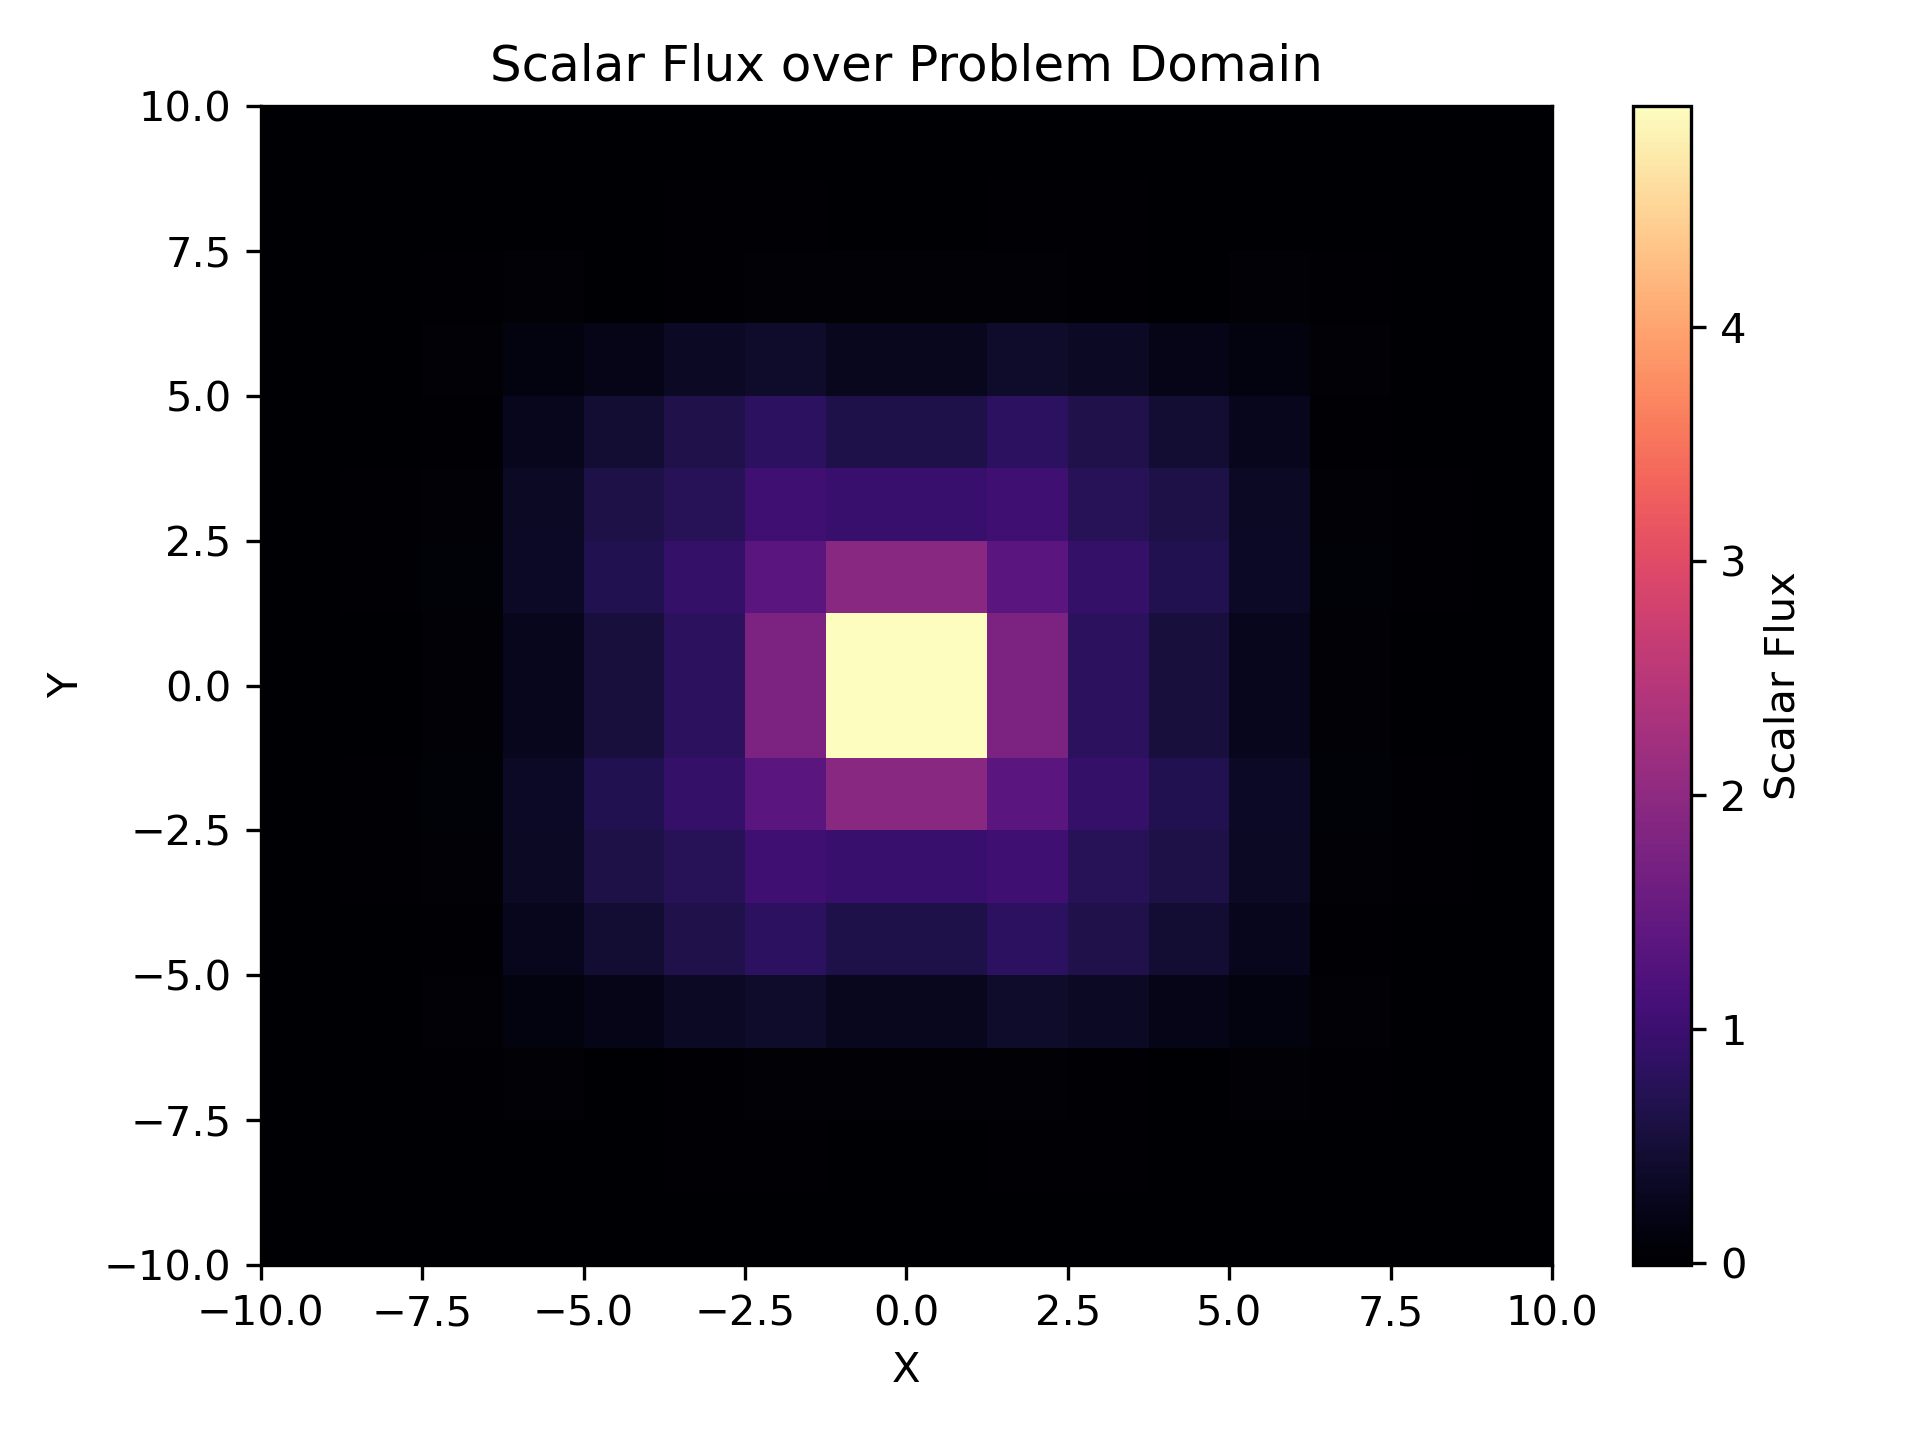
\includegraphics[width=0.65\textwidth]{figures/absorbing/cell_fluxes_256_8.png}
      \subcaption{$N=256$}
    \end{subfigure}%
    \begin{subfigure}{.5\textwidth}
      \centering
      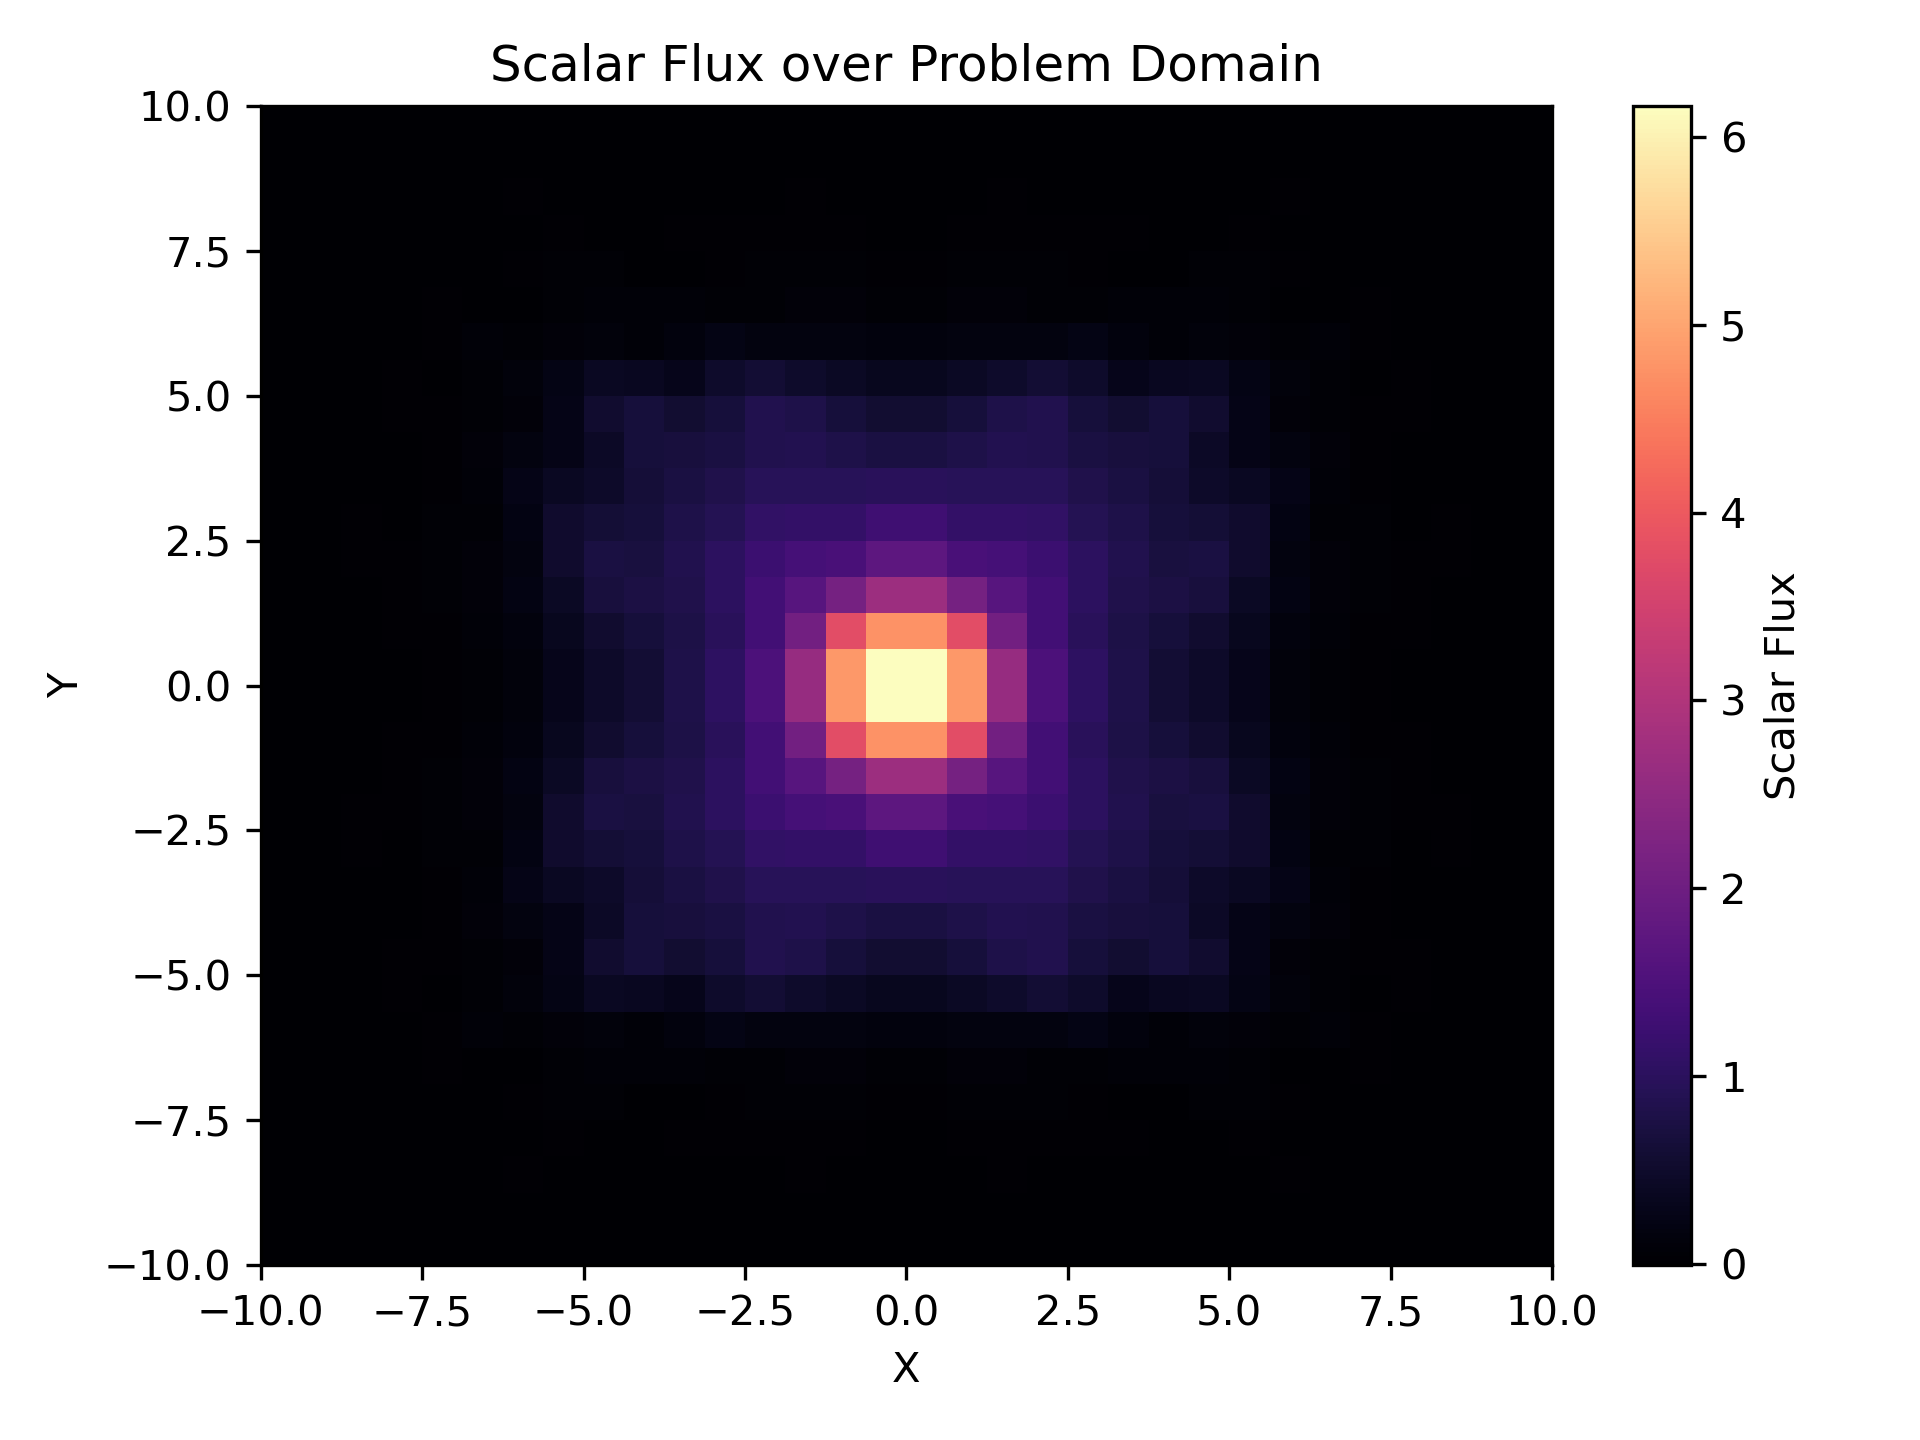
\includegraphics[width=0.65\textwidth]{figures/absorbing/cell_fluxes_1024_8.png}
      \subcaption{$N=1024$}
    \end{subfigure}
    \begin{subfigure}{.5\textwidth}
      \centering
      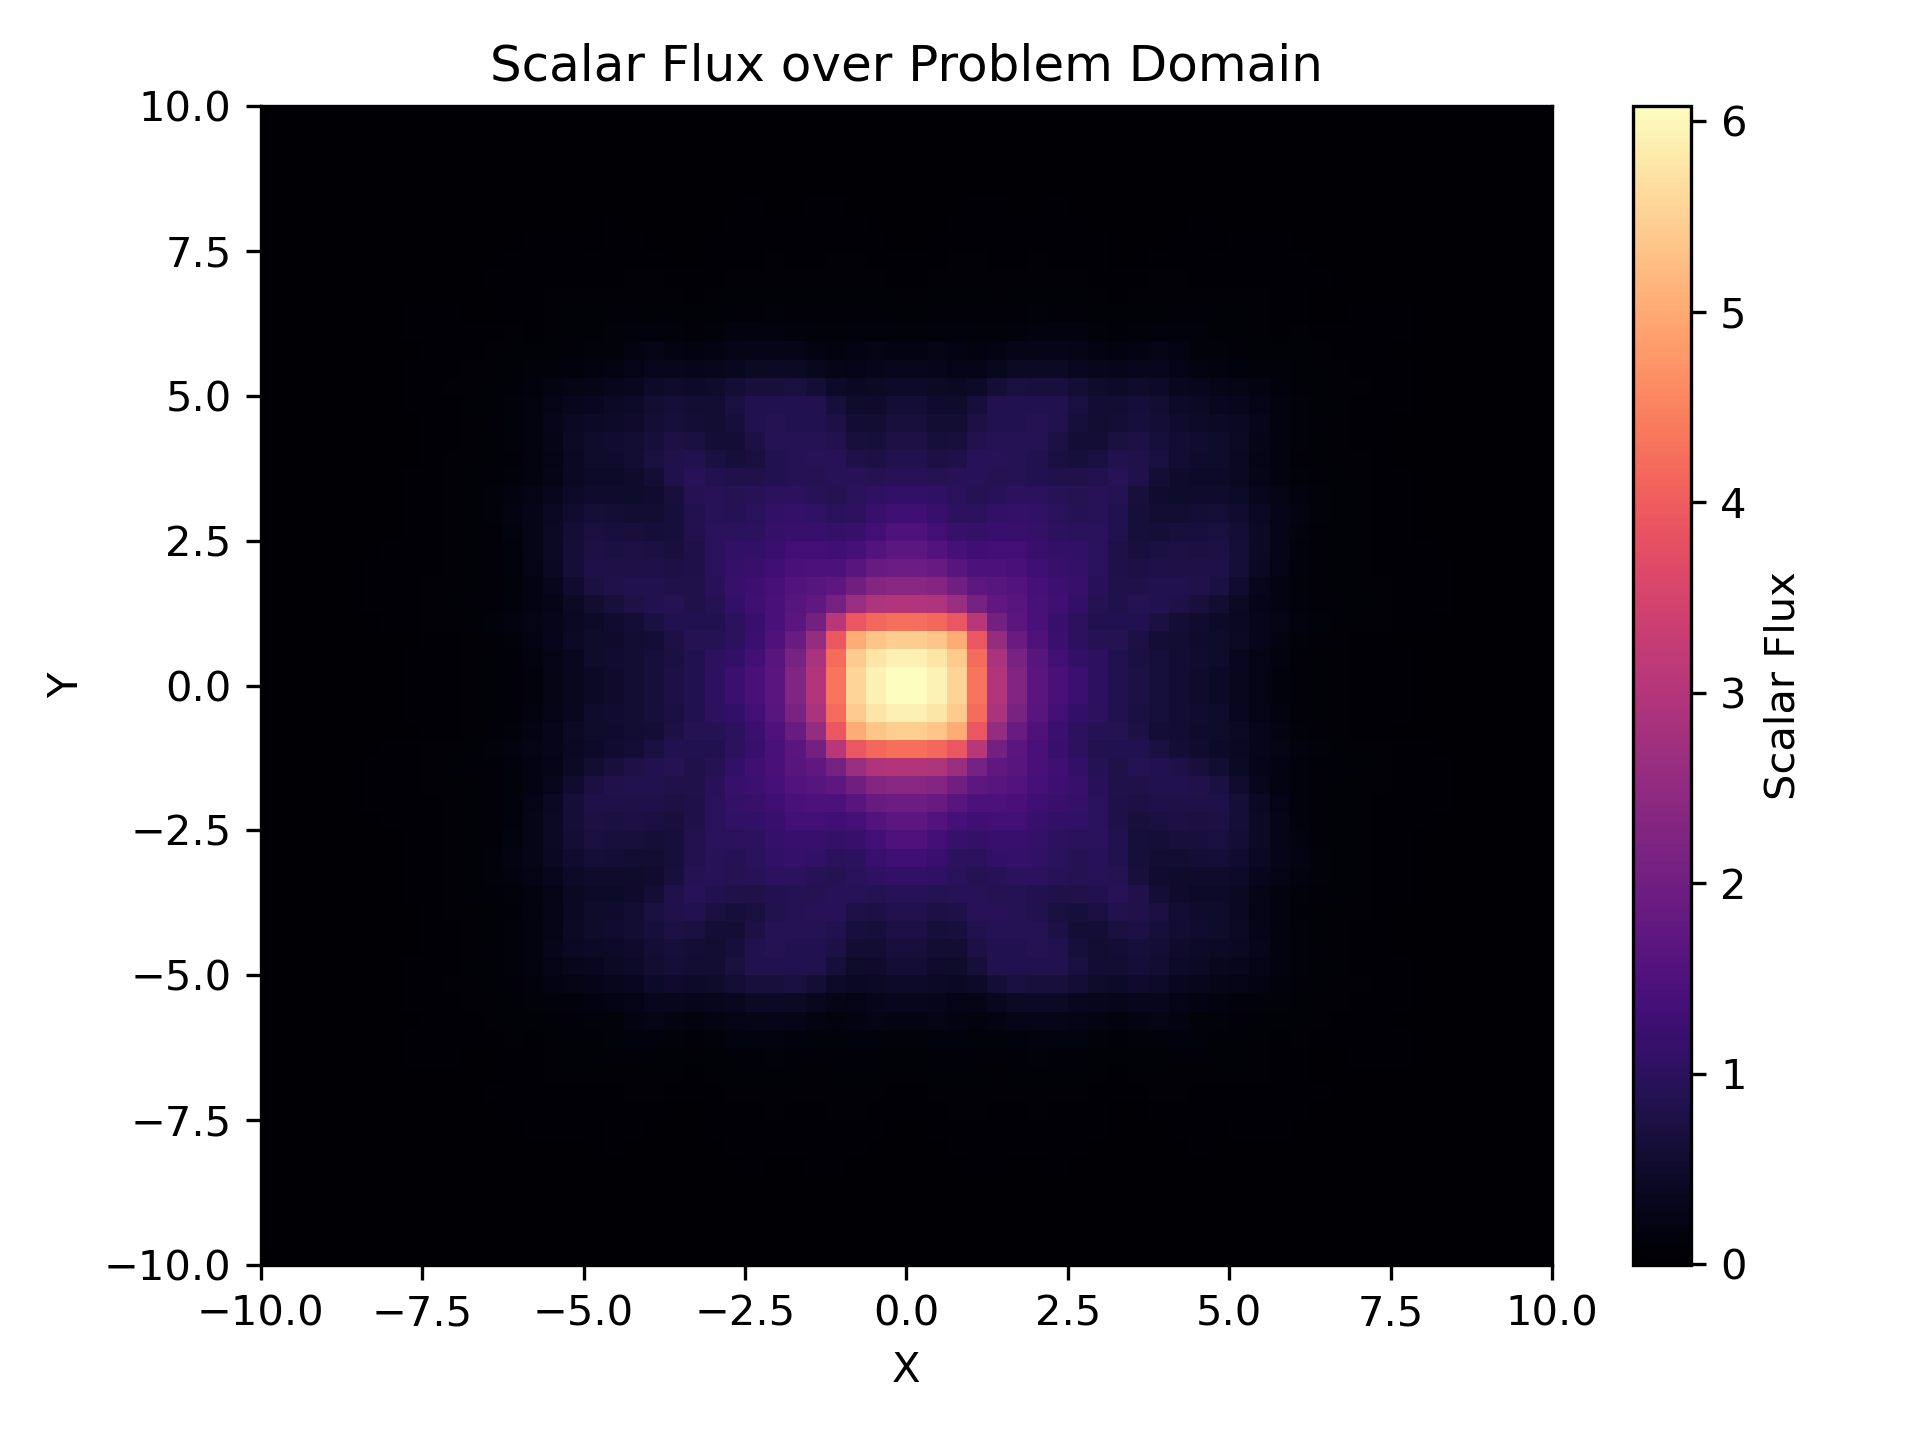
\includegraphics[width=0.65\textwidth]{figures/absorbing/cell_fluxes_4096_8.png}
      \subcaption{$N=4096$}
    \end{subfigure}%
    \begin{subfigure}{.5\textwidth}
      \centering
      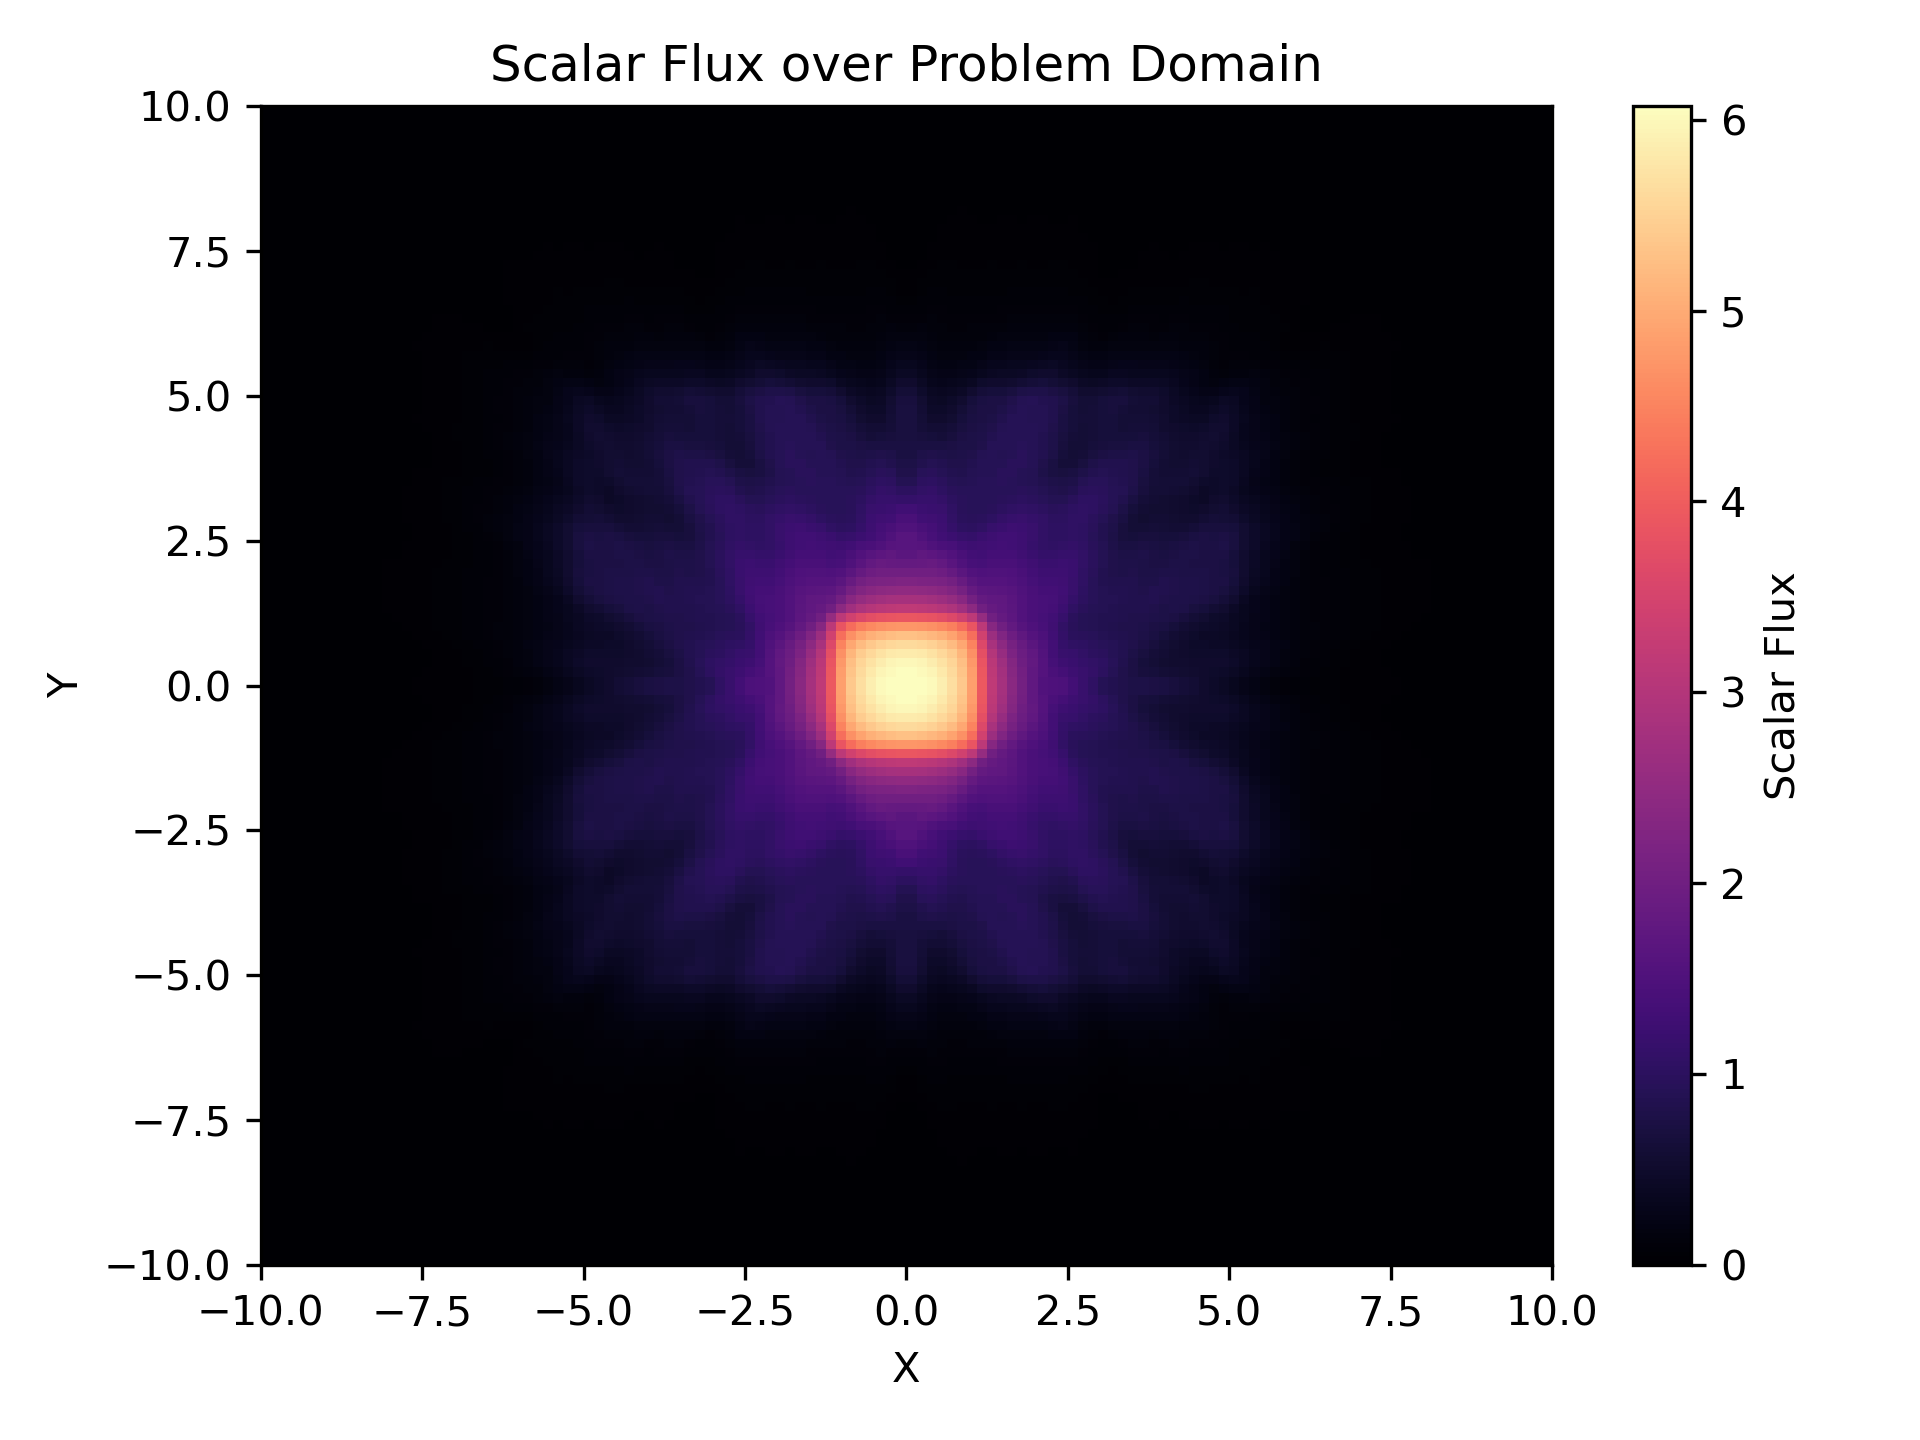
\includegraphics[width=0.65\textwidth]{figures/absorbing/cell_fluxes_16384_8.png}
      \subcaption{$N=16384$}
    \end{subfigure}
    \caption{Solution of absorbing \glspl{arp1} for varying $N$ with $S_{8}$.}
  \end{figure}
\end{frame}

\begin{frame}
  \frametitle{\glspl{arp1} Absorbing Medium Results}
  \begin{figure}[b]
    \centering
    \begin{subfigure}{.5\textwidth}
      \centering
      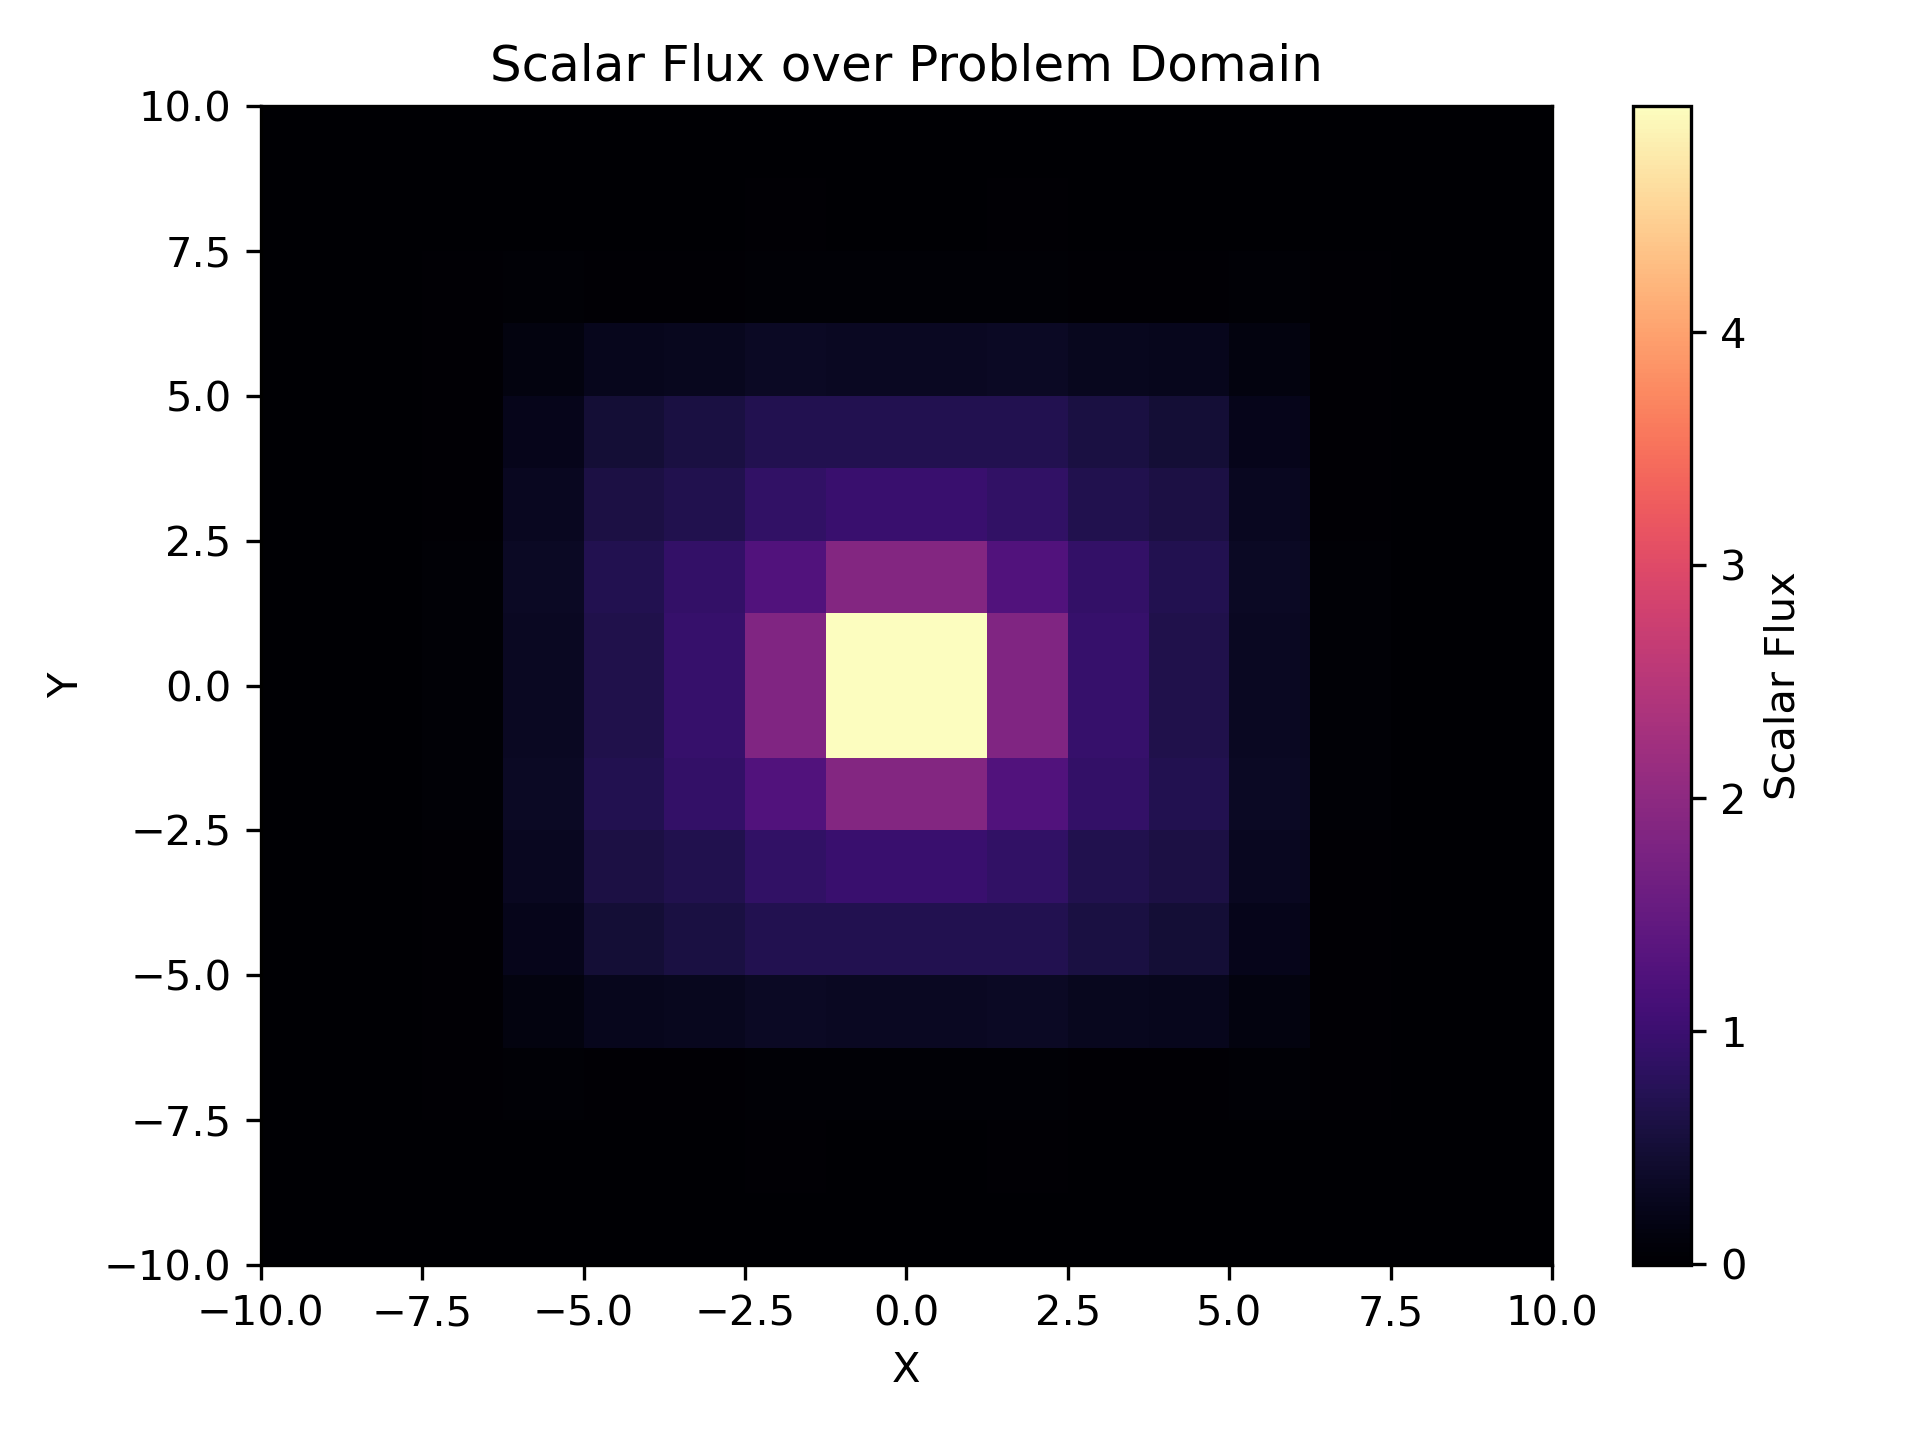
\includegraphics[width=0.65\textwidth]{figures/absorbing/cell_fluxes_256_16.png}
      \subcaption{$N=256$}
    \end{subfigure}%
    \begin{subfigure}{.5\textwidth}
      \centering
      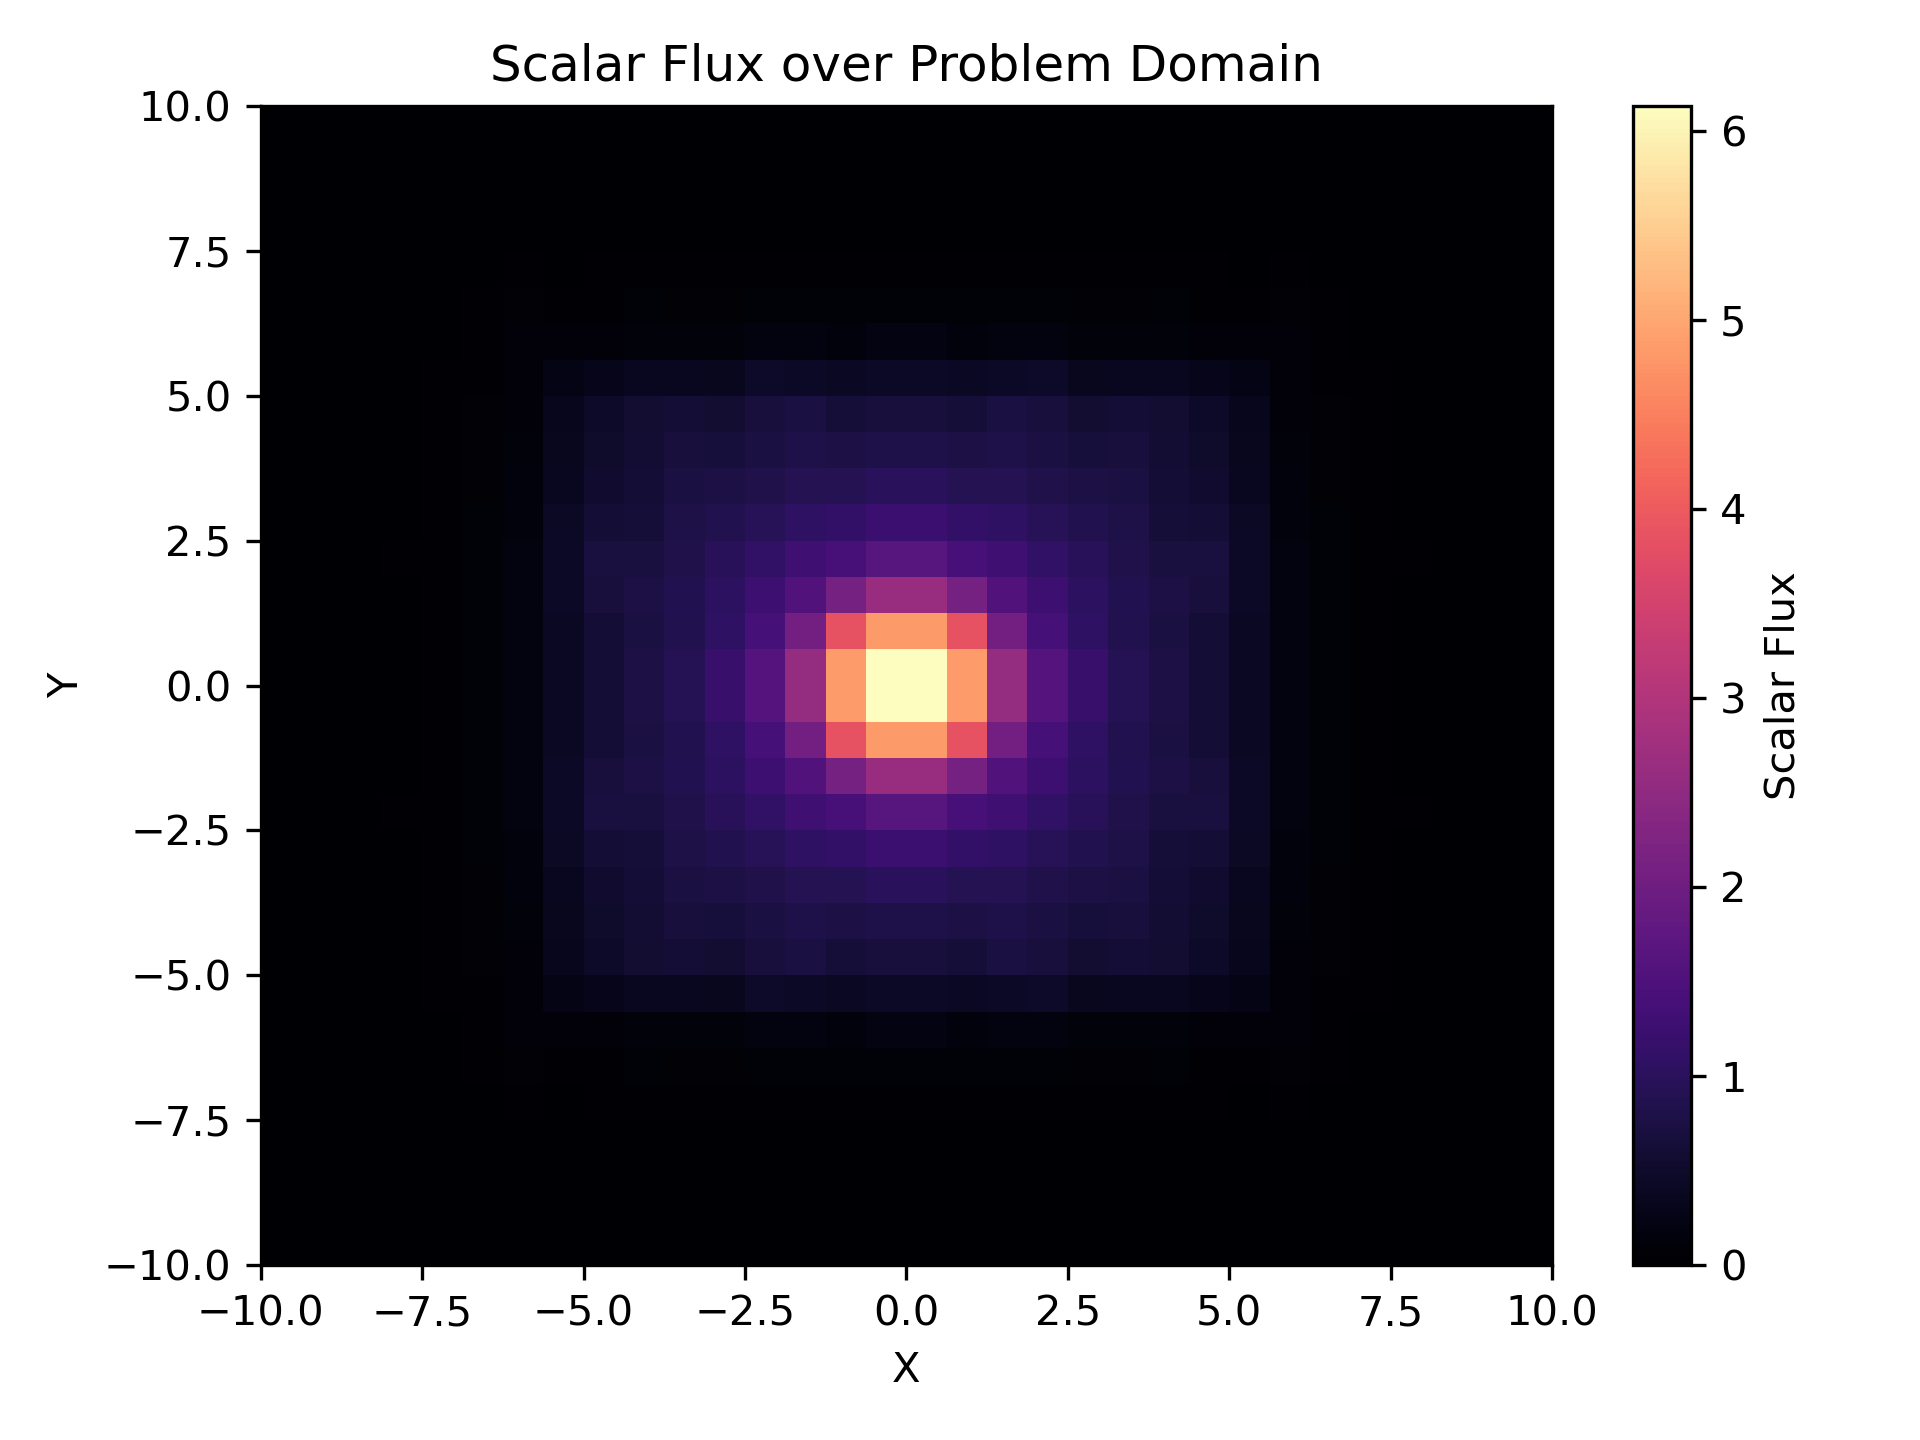
\includegraphics[width=0.65\textwidth]{figures/absorbing/cell_fluxes_1024_16.png}
      \subcaption{$N=1024$}
    \end{subfigure}
    \begin{subfigure}{.5\textwidth}
      \centering
      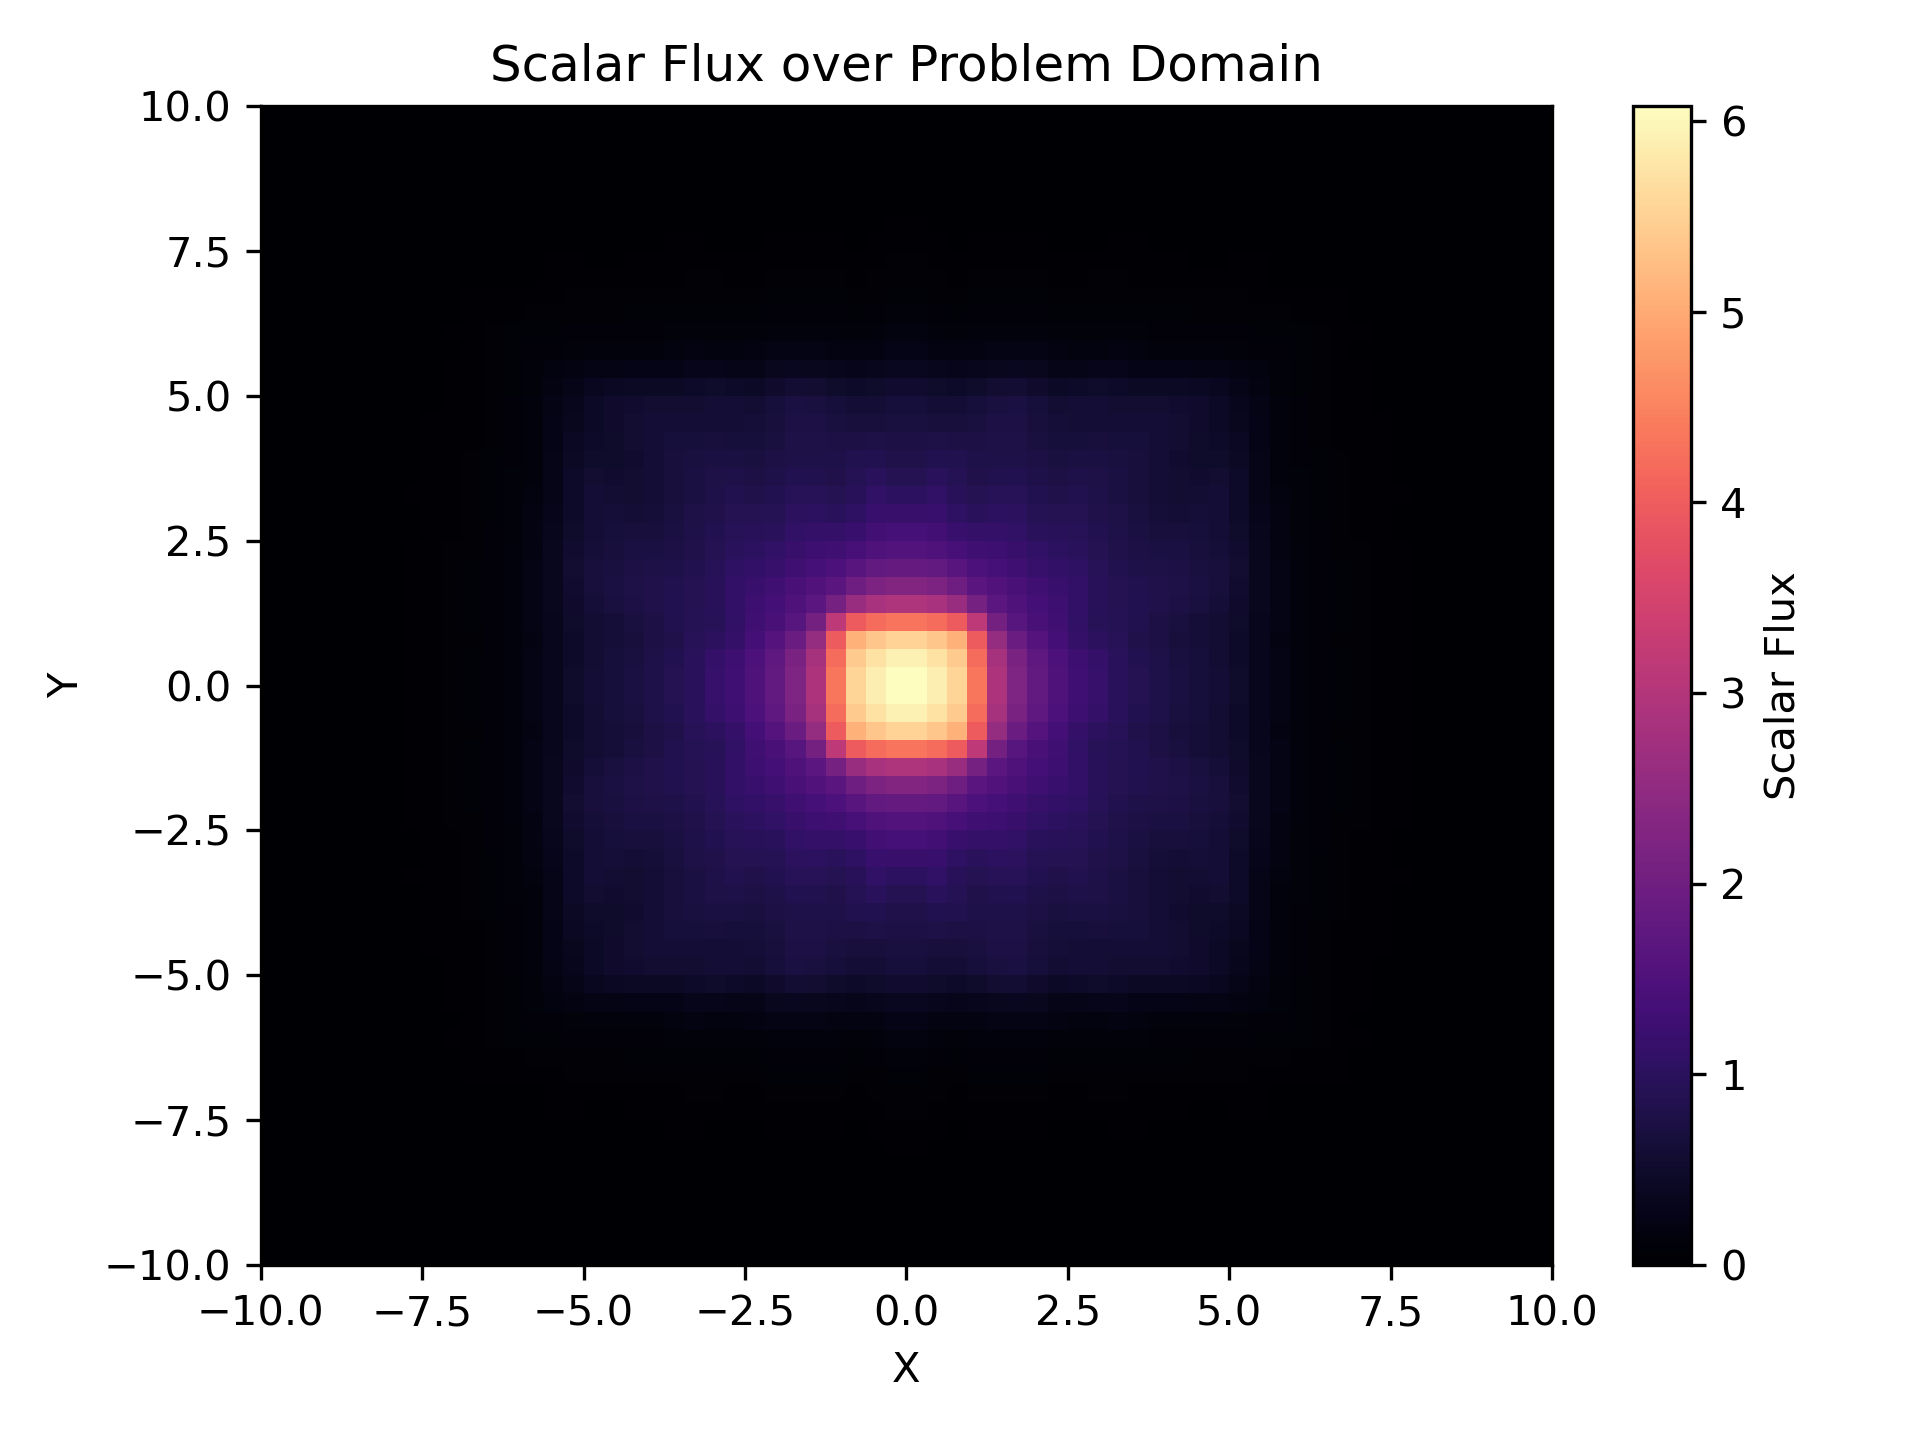
\includegraphics[width=0.65\textwidth]{figures/absorbing/cell_fluxes_4096_16.png}
      \subcaption{$N=4096$}
    \end{subfigure}%
    \begin{subfigure}{.5\textwidth}
      \centering
      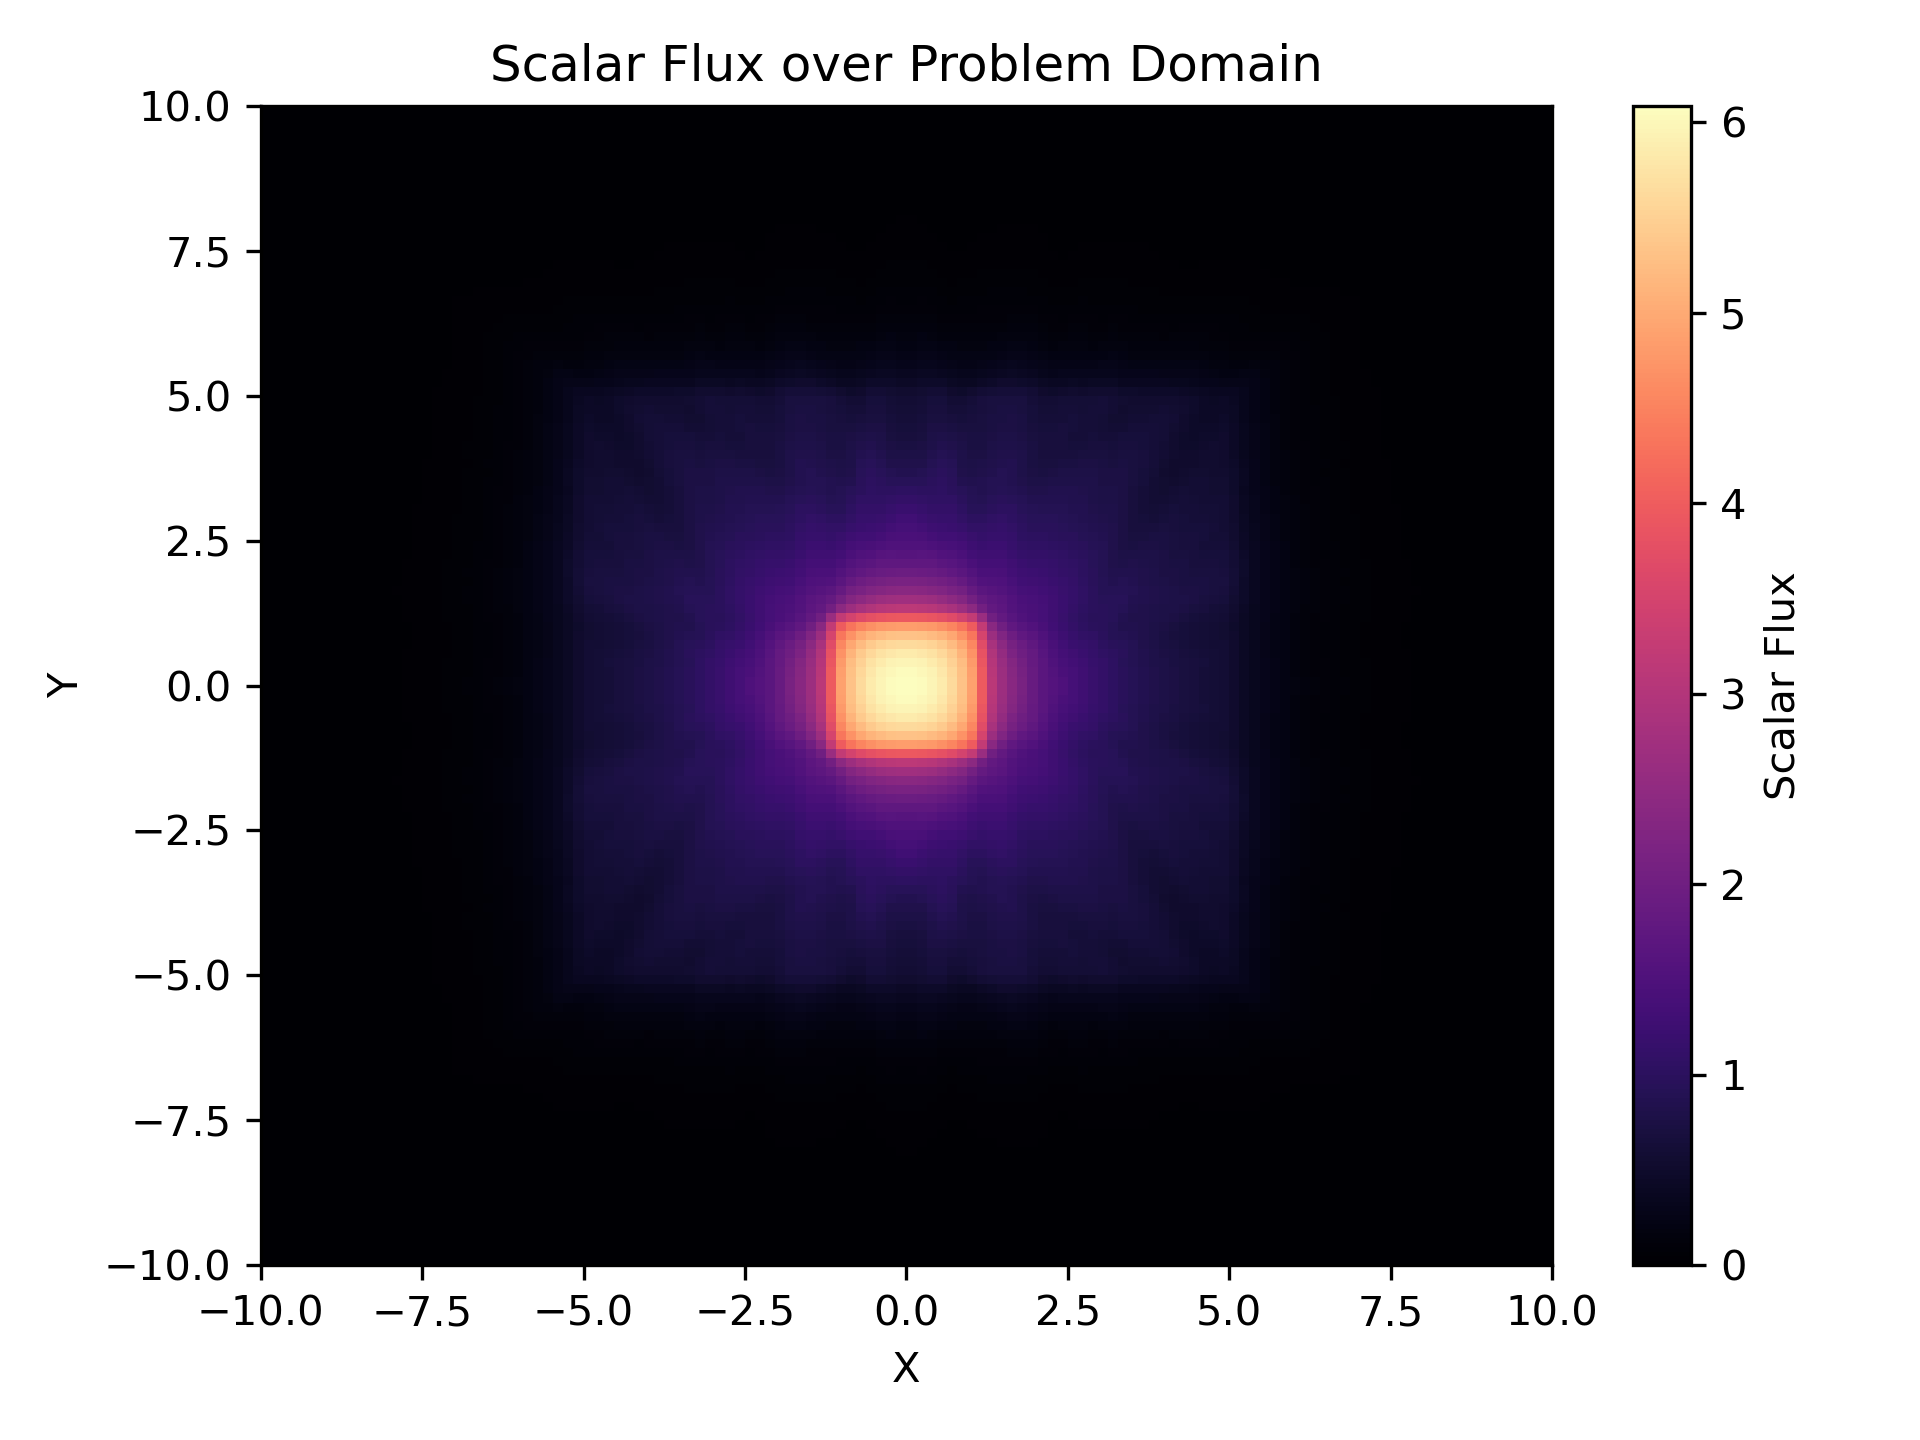
\includegraphics[width=0.65\textwidth]{figures/absorbing/cell_fluxes_16384_16.png}
      \subcaption{$N=16384$}
    \end{subfigure}
    \caption{Solution of absorbing \glspl{arp1} for varying $N$ with $S_{16}$.}
  \end{figure}
\end{frame}

\begin{frame}
  \frametitle{\glspl{arp1} Absorbing Medium Results}
  \begin{figure}[b]
    \centering
    \begin{subfigure}{.5\textwidth}
      \centering
      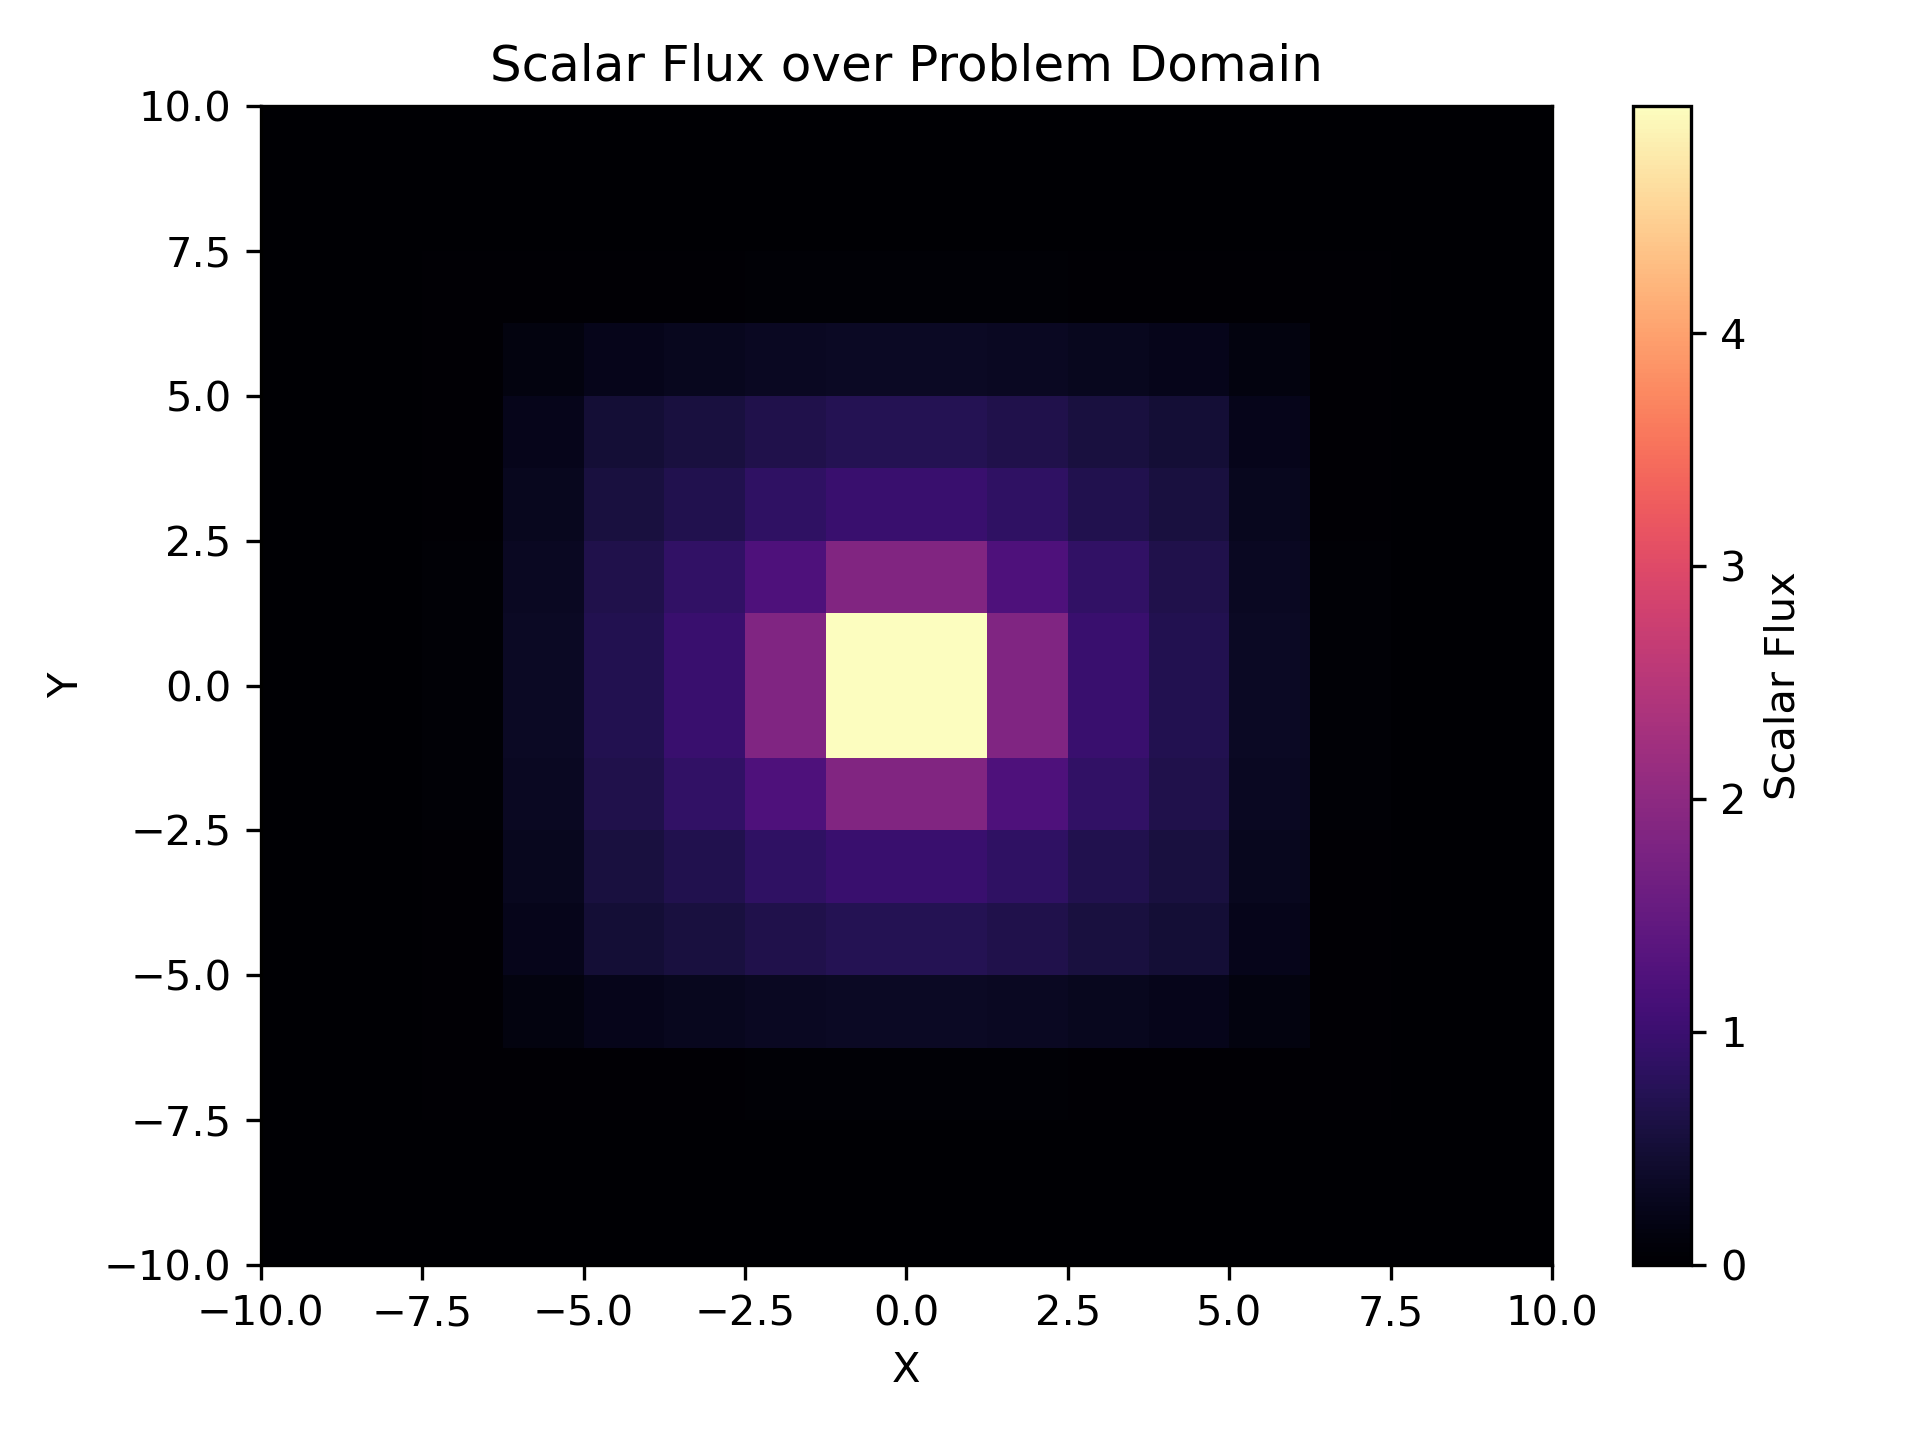
\includegraphics[width=0.65\textwidth]{figures/absorbing/cell_fluxes_256_32.png}
      \subcaption{$N=256$}
    \end{subfigure}%
    \begin{subfigure}{.5\textwidth}
      \centering
      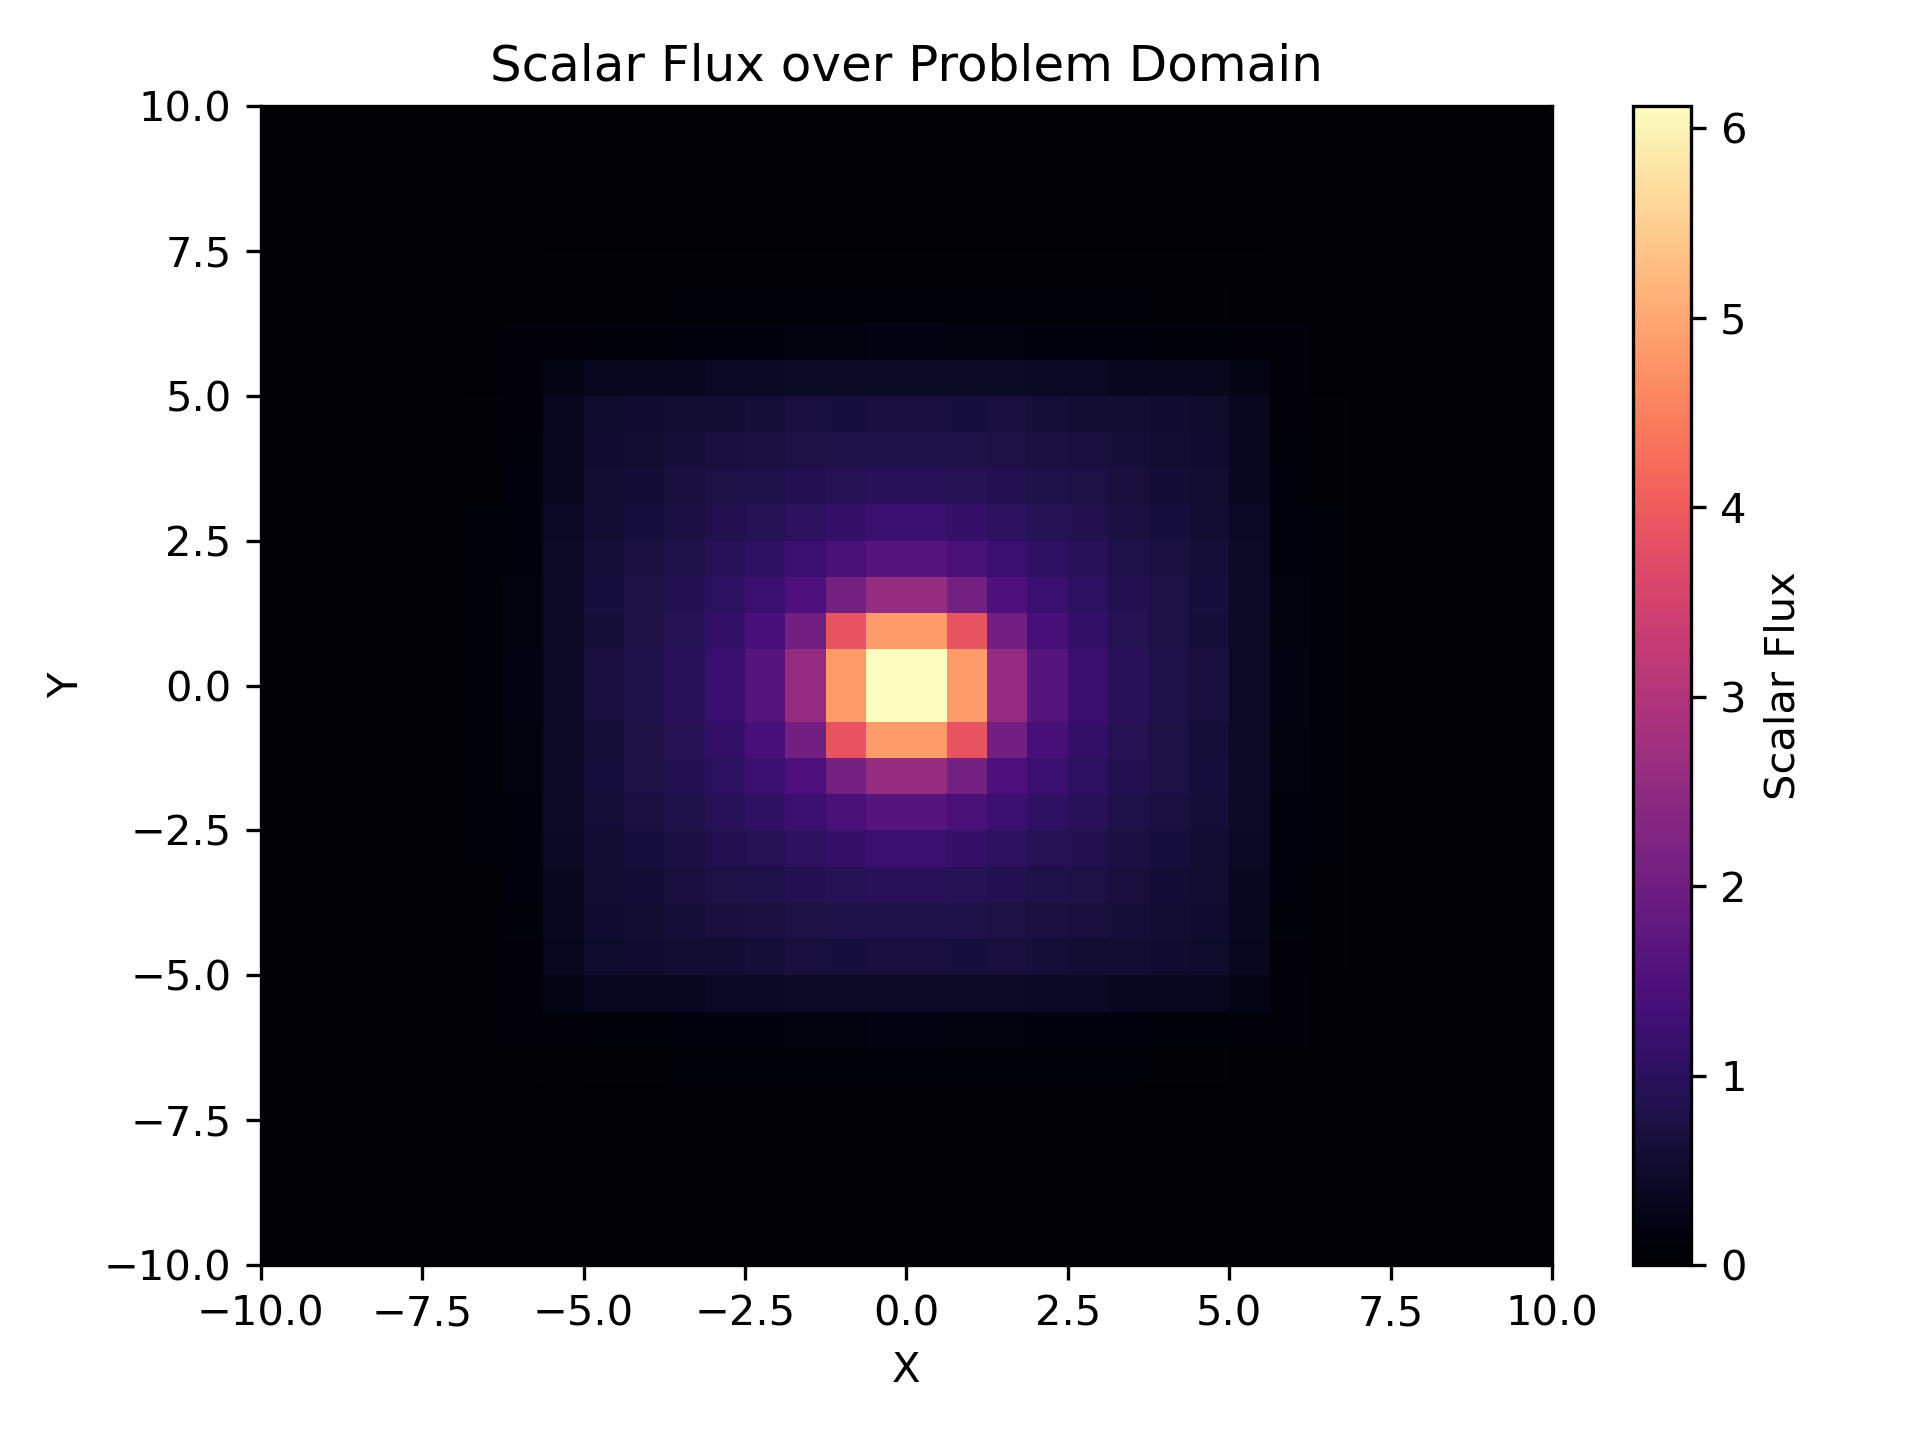
\includegraphics[width=0.65\textwidth]{figures/absorbing/cell_fluxes_1024_32.png}
      \subcaption{$N=1024$}
    \end{subfigure}
    \begin{subfigure}{.5\textwidth}
      \centering
      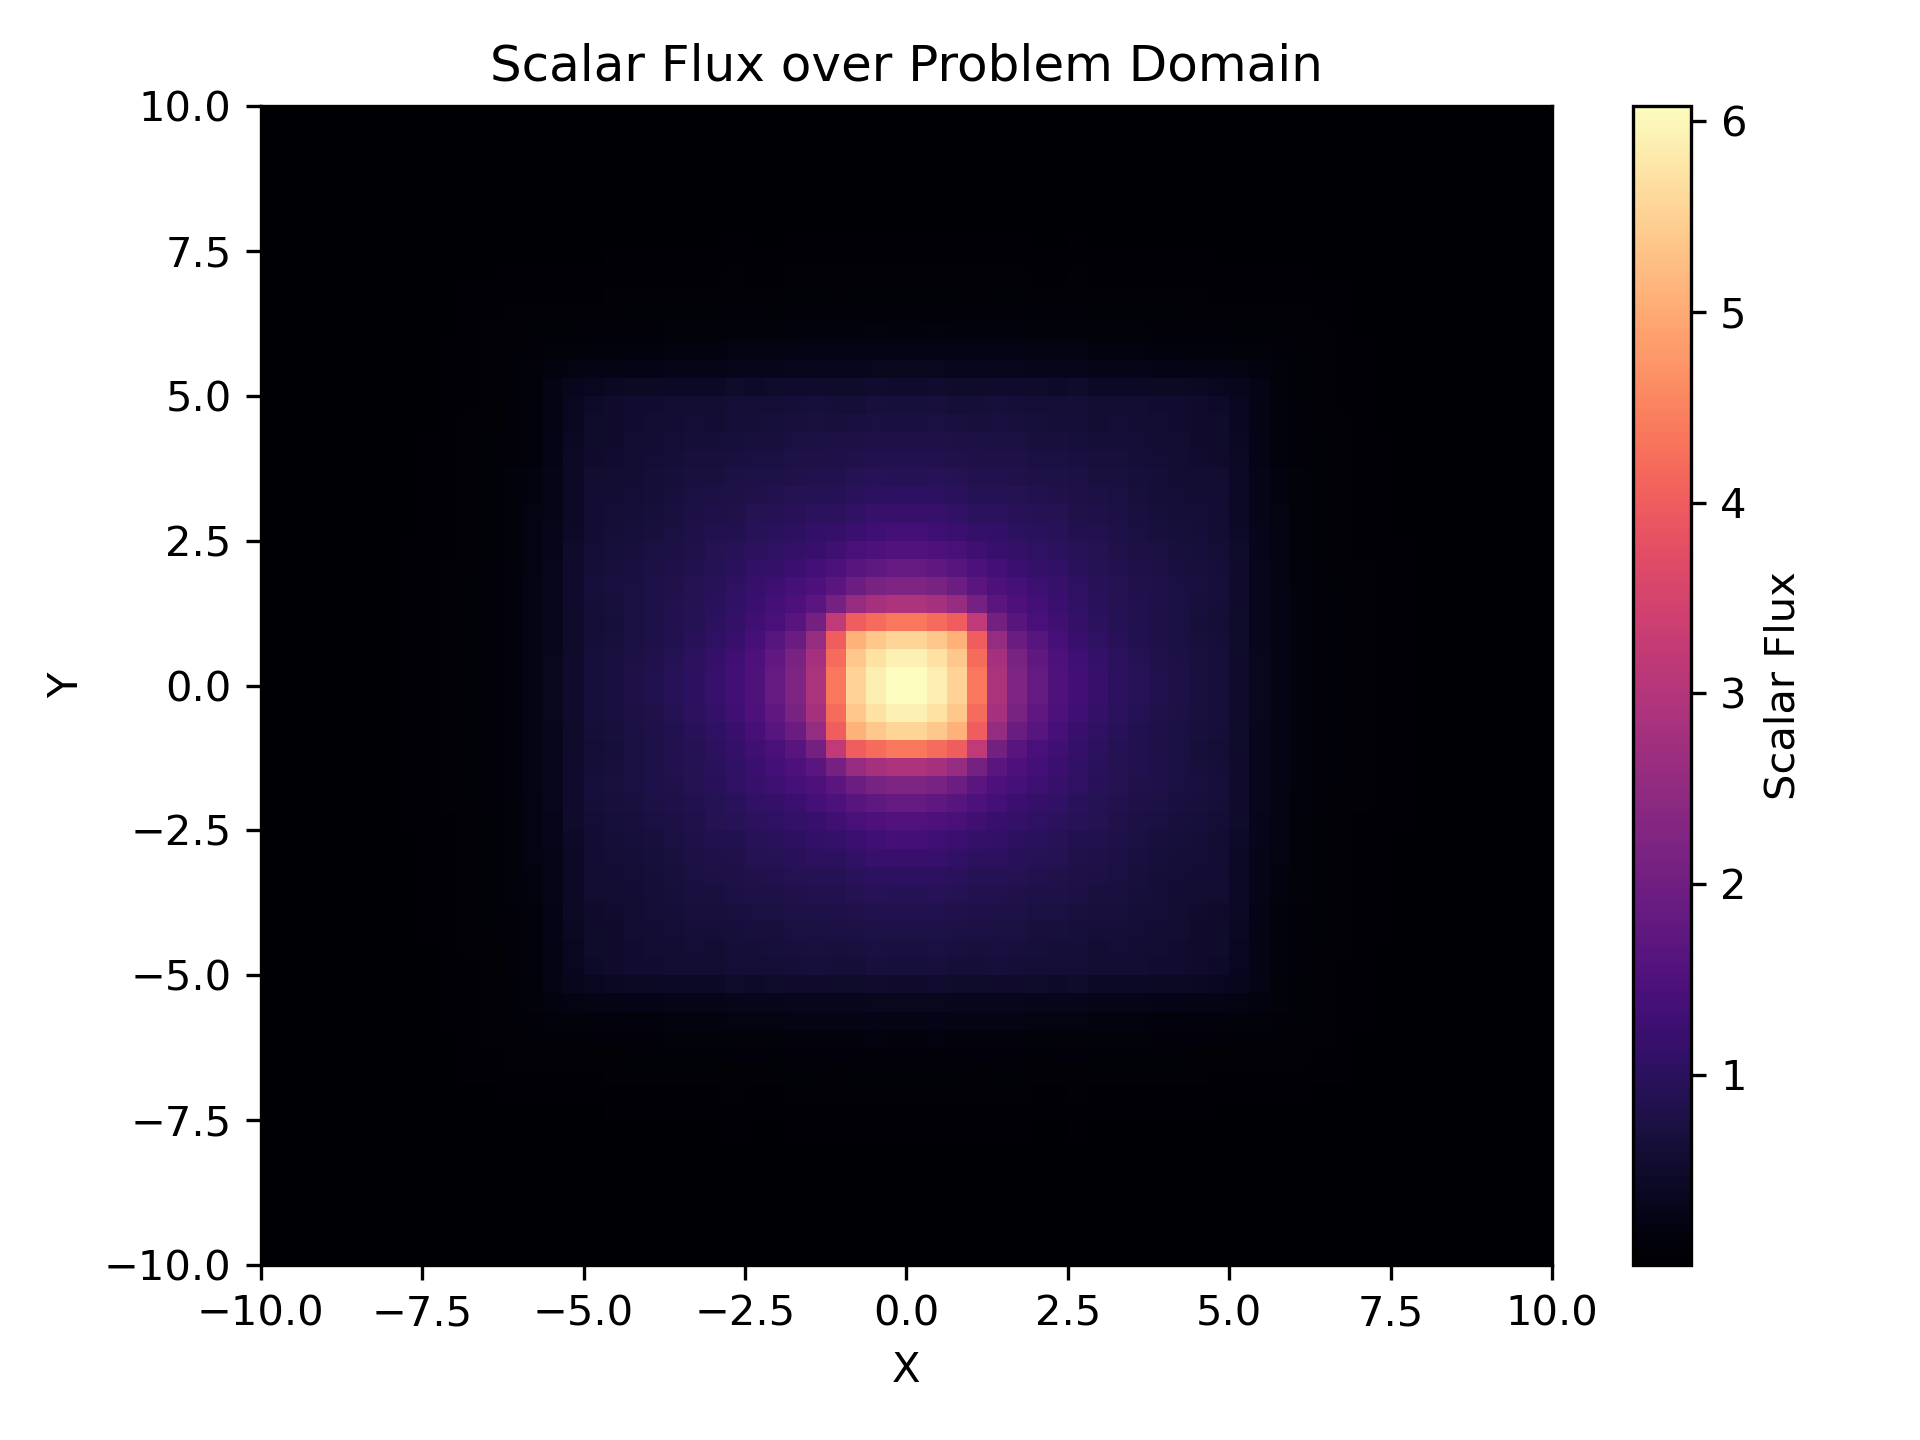
\includegraphics[width=0.65\textwidth]{figures/absorbing/cell_fluxes_4096_32.png}
      \subcaption{$N=4096$}
    \end{subfigure}%
    \begin{subfigure}{.5\textwidth}
      \centering
      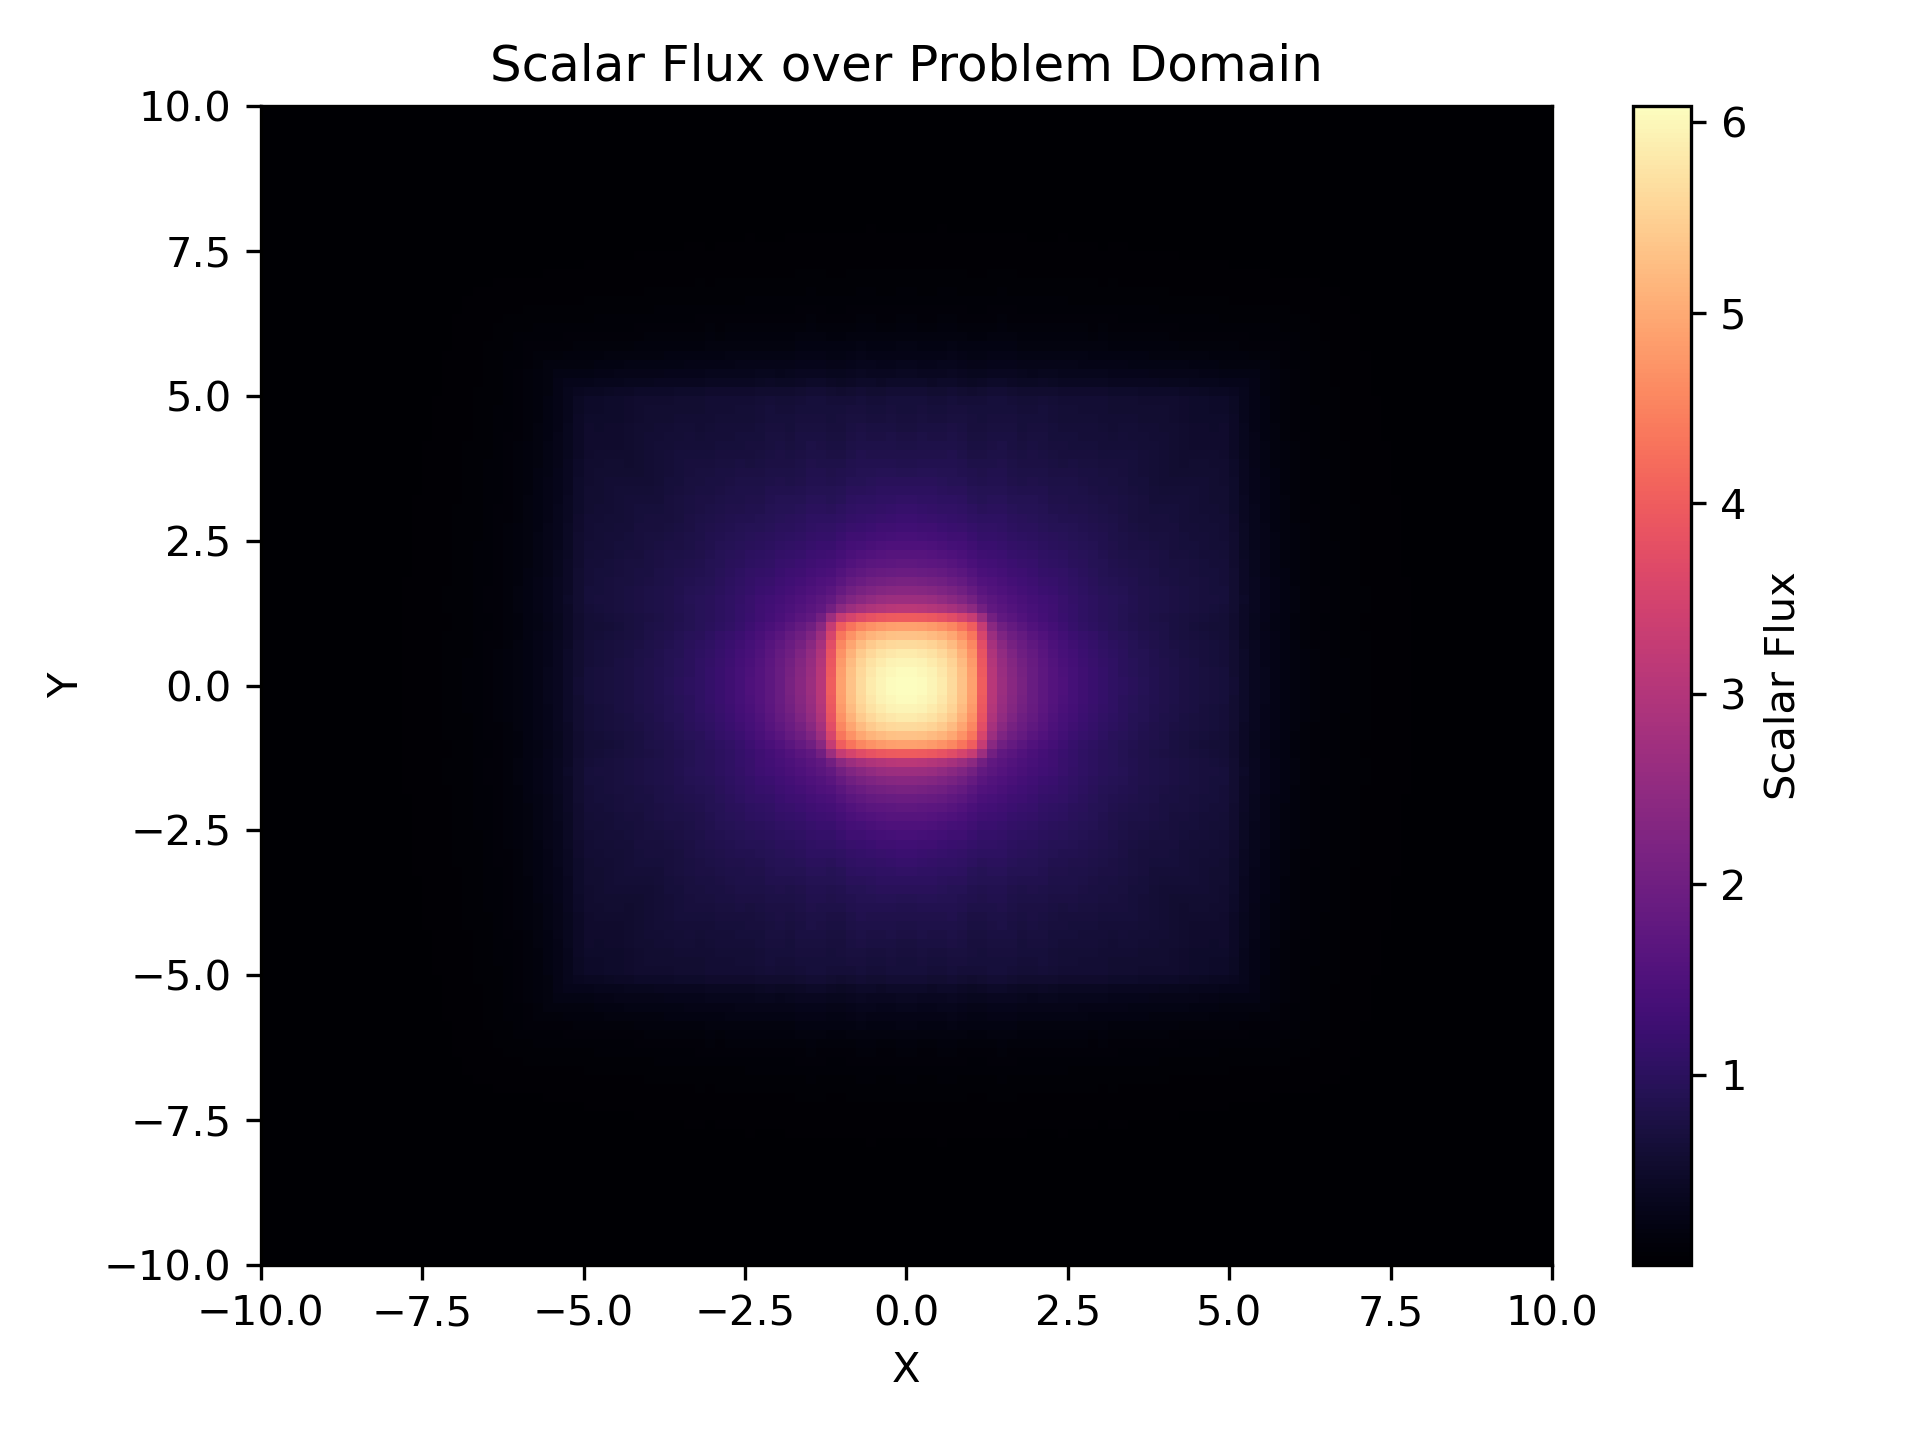
\includegraphics[width=0.65\textwidth]{figures/absorbing/cell_fluxes_16384_32.png}
      \subcaption{$N=16384$}
    \end{subfigure}
    \caption{Solution of absorbing \glspl{arp1} for varying $N$ with $S_{32}$.}
  \end{figure}
\end{frame}

\begin{frame}
  \frametitle{\glspl{arp1} Absorbing Medium Results}
  \begin{figure}[b]
    \centering
    \begin{subfigure}{.5\textwidth}
      \centering
      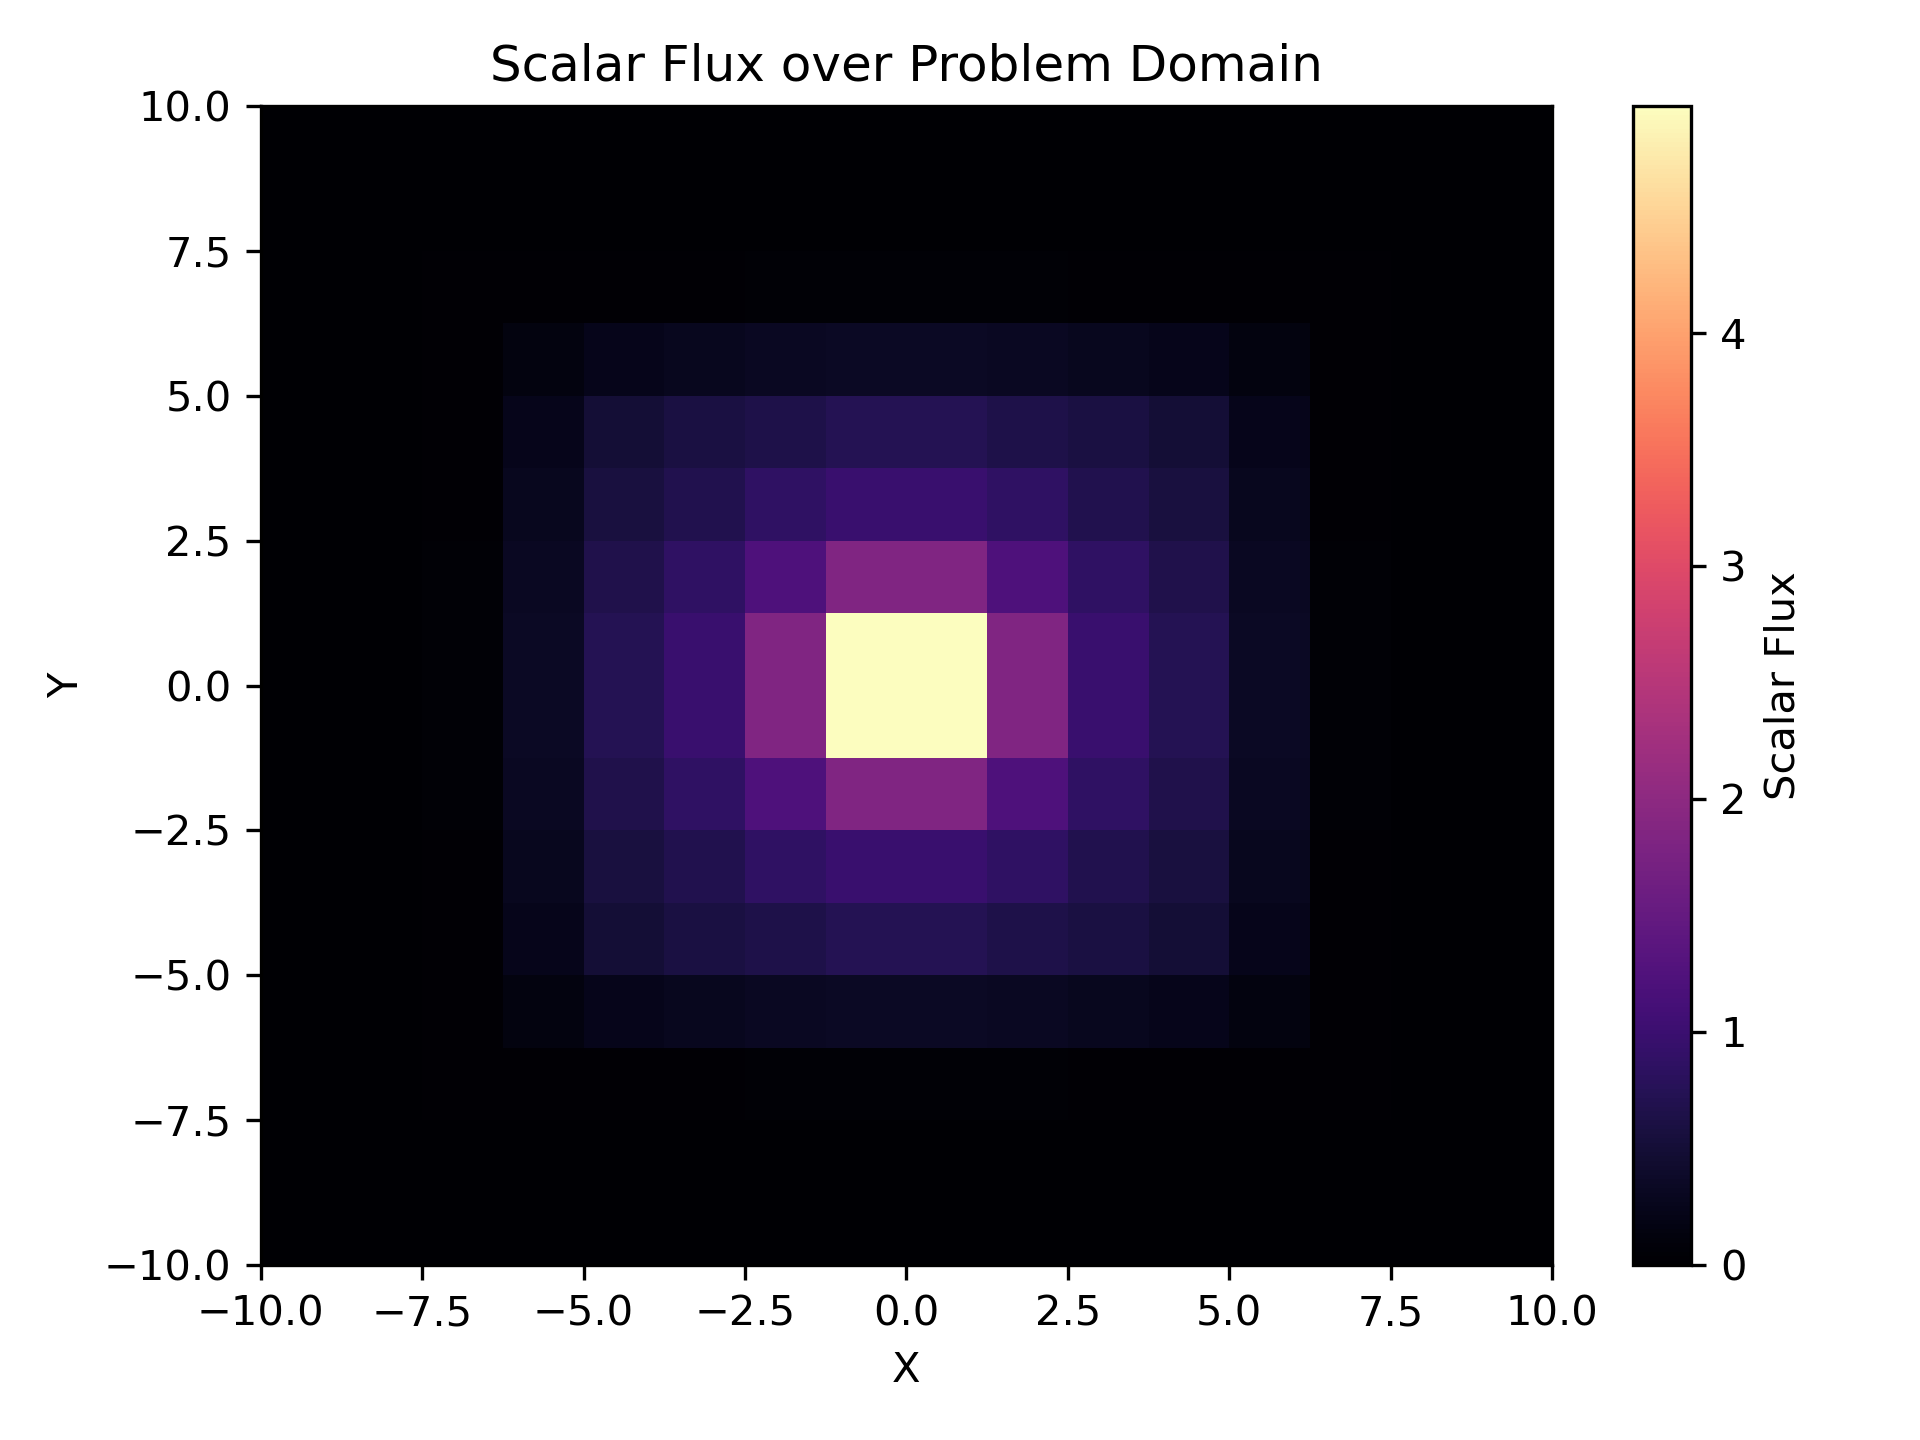
\includegraphics[width=0.65\textwidth]{figures/absorbing/cell_fluxes_256_64.png}
      \subcaption{$N=256$}
    \end{subfigure}%
    \begin{subfigure}{.5\textwidth}
      \centering
      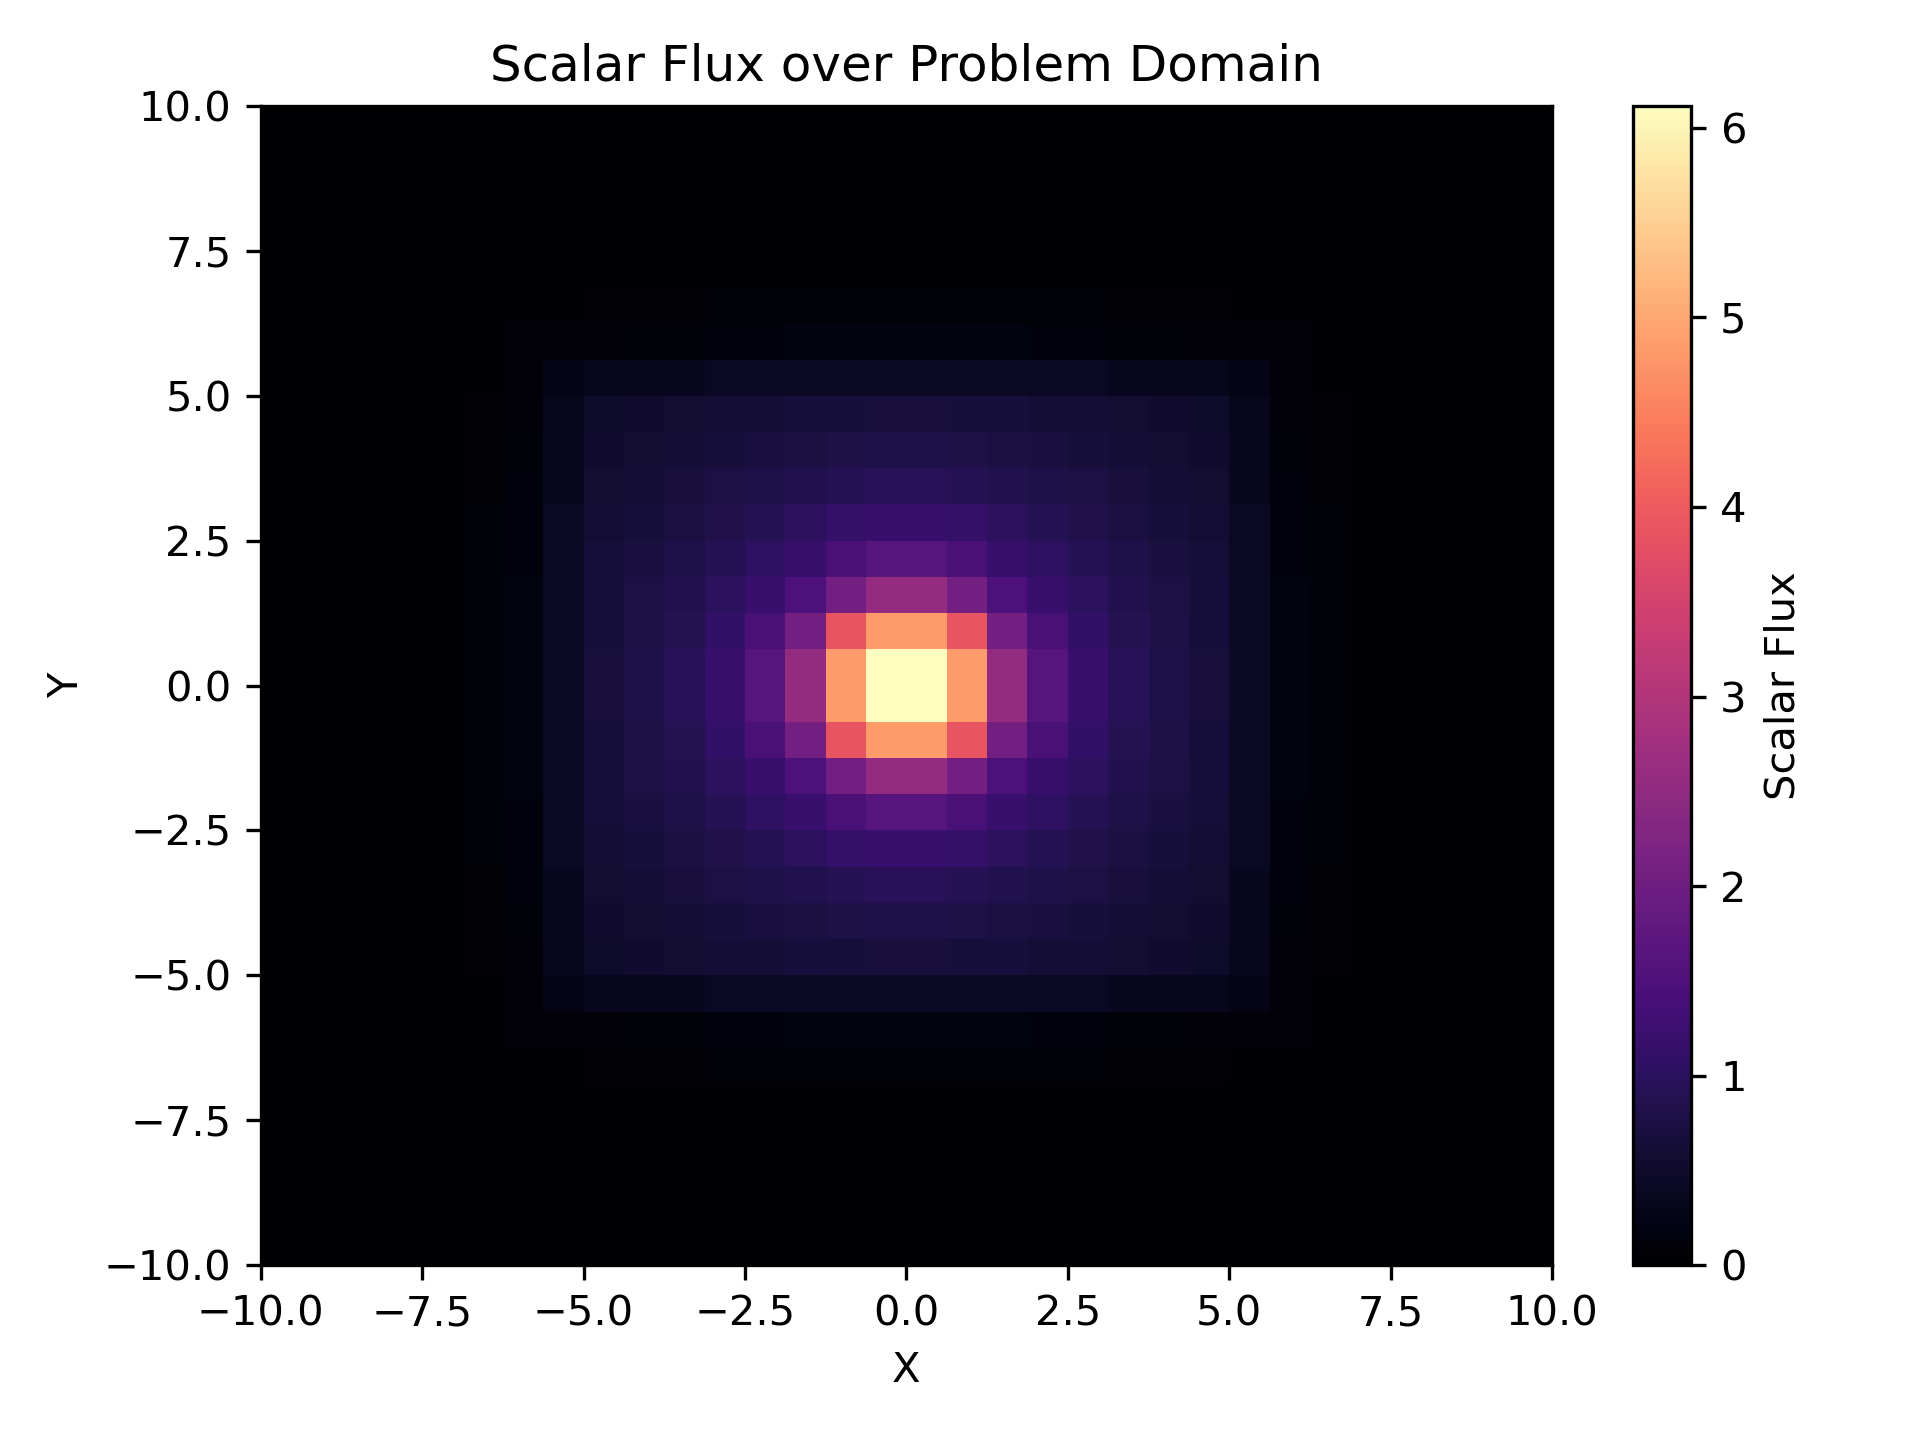
\includegraphics[width=0.65\textwidth]{figures/absorbing/cell_fluxes_1024_64.png}
      \subcaption{$N=1024$}
    \end{subfigure}
    \begin{subfigure}{.5\textwidth}
      \centering
      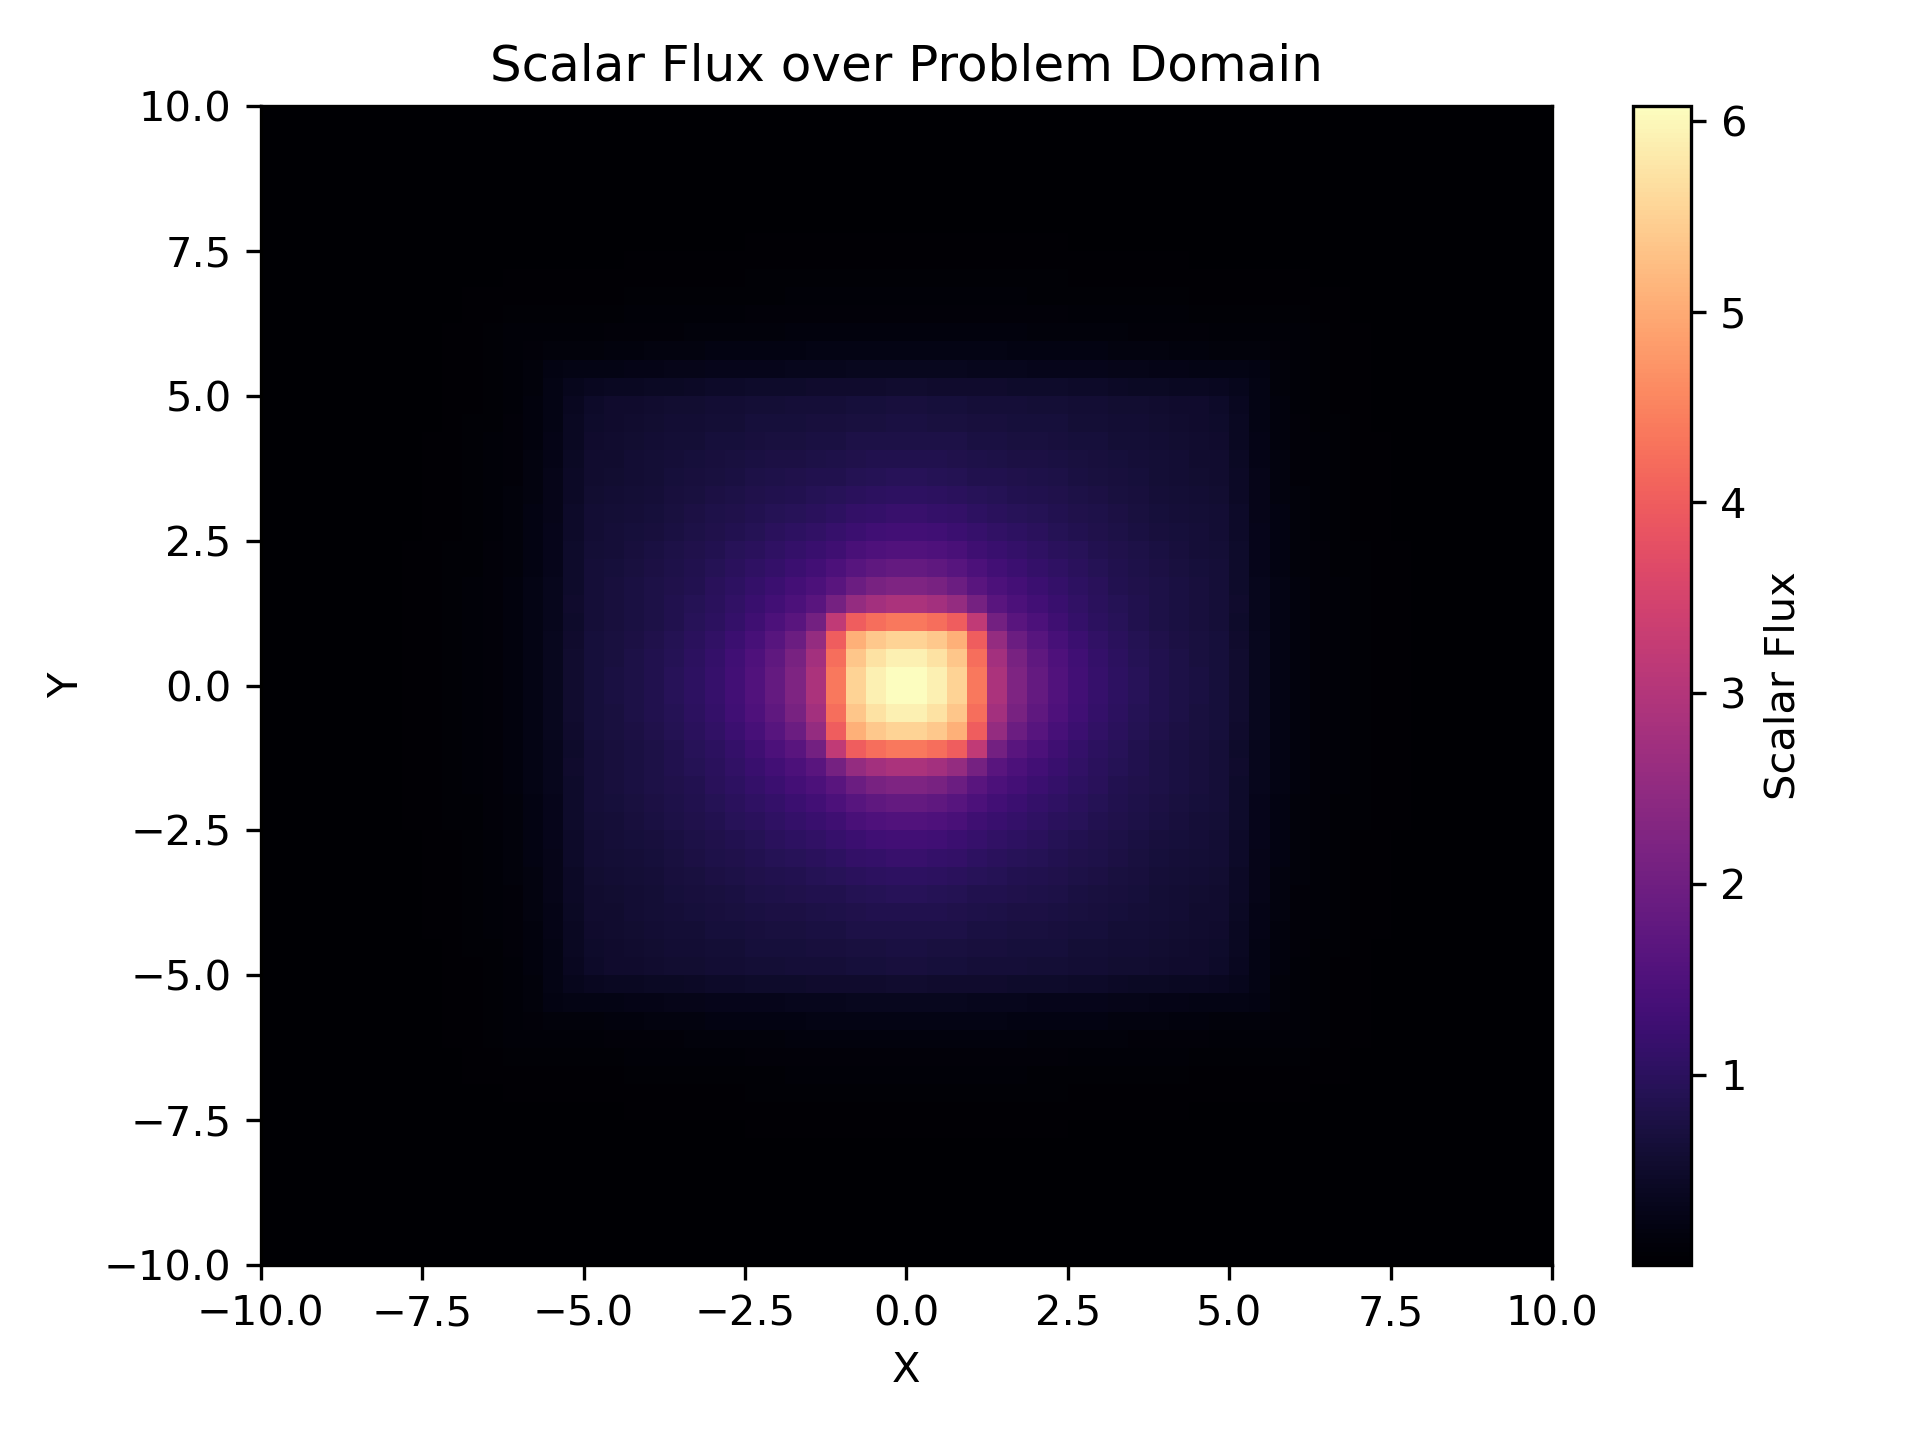
\includegraphics[width=0.65\textwidth]{figures/absorbing/cell_fluxes_4096_64.png}
      \subcaption{$N=4096$}
    \end{subfigure}%
    \begin{subfigure}{.5\textwidth}
      \centering
      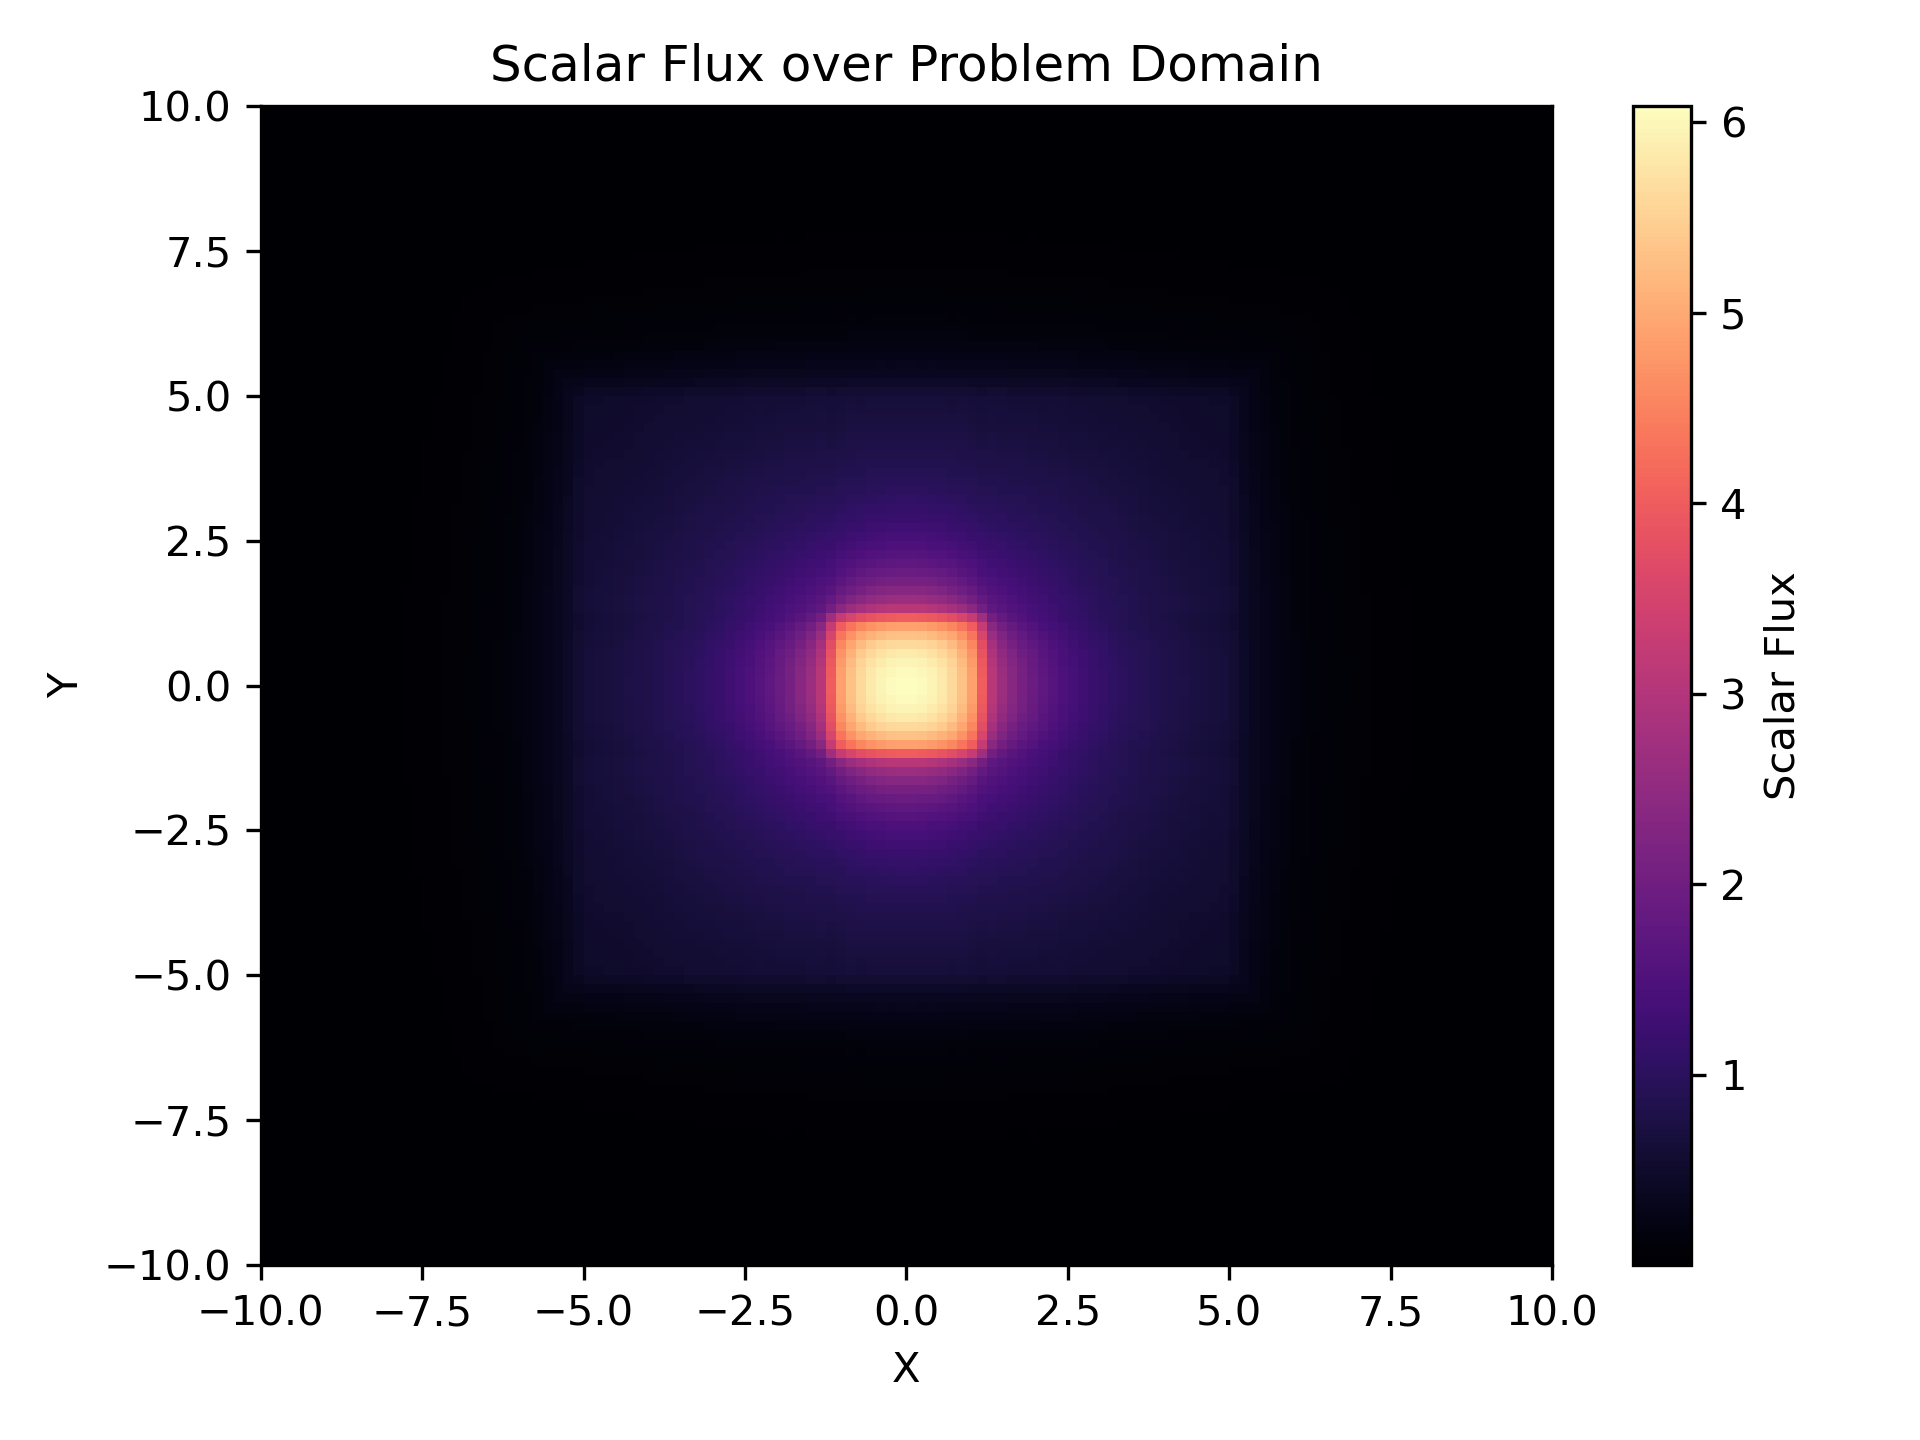
\includegraphics[width=0.65\textwidth]{figures/absorbing/cell_fluxes_16384_64.png}
      \subcaption{$N=16384$}
    \end{subfigure}
    \caption{Solution of absorbing \glspl{arp1} for varying $N$ with $S_{64}$.}
  \end{figure}
\end{frame}


\begin{frame}
  \frametitle{\glspl{arp1} Scattering Medium Results}
  \begin{figure}[b]
    \centering
    \begin{subfigure}{.5\textwidth}
      \centering
      
\includegraphics[width=0.65\textwidth]{figures/scattering/cell_fluxes_256_8.png}
      \subcaption{$N=256$}
    \end{subfigure}%
    \begin{subfigure}{.5\textwidth}
      \centering
      
\includegraphics[width=0.65\textwidth]{figures/scattering/cell_fluxes_1024_8.png}
      \subcaption{$N=1024$}
    \end{subfigure}
    \begin{subfigure}{.5\textwidth}
      \centering
      
\includegraphics[width=0.65\textwidth]{figures/scattering/cell_fluxes_4096_8.png}
      \subcaption{$N=4096$}
    \end{subfigure}%
    \begin{subfigure}{.5\textwidth}
      \centering
      
\includegraphics[width=0.65\textwidth]{figures/scattering/cell_fluxes_16384_8.png}
      \subcaption{$N=16384$}
    \end{subfigure}
    \caption{Solution of scattering \glspl{arp1} for varying $N$ with $S_{8}$.}
  \end{figure}
\end{frame}

\begin{frame}
  \frametitle{\glspl{arp1} Scattering Medium Results}
  \begin{figure}[b]
    \centering
    \begin{subfigure}{.5\textwidth}
      \centering
      
\includegraphics[width=0.65\textwidth]{figures/scattering/cell_fluxes_256_16.png}
      \subcaption{$N=256$}
    \end{subfigure}%
    \begin{subfigure}{.5\textwidth}
      \centering
      
\includegraphics[width=0.65\textwidth]{figures/scattering/cell_fluxes_1024_16.png}
      \subcaption{$N=1024$}
    \end{subfigure}
    \begin{subfigure}{.5\textwidth}
      \centering
      
\includegraphics[width=0.65\textwidth]{figures/scattering/cell_fluxes_4096_16.png}
      \subcaption{$N=4096$}
    \end{subfigure}%
    \begin{subfigure}{.5\textwidth}
      \centering
      
\includegraphics[width=0.65\textwidth]{figures/scattering/cell_fluxes_16384_16.png}
      \subcaption{$N=16384$}
    \end{subfigure}
    \caption{Solution of scattering \glspl{arp1} for varying $N$ with $S_{16}$.}
  \end{figure}
\end{frame}

\begin{frame}
  \frametitle{\glspl{arp1} Scattering Medium Results}
  \begin{figure}[b]
    \centering
    \begin{subfigure}{.5\textwidth}
      \centering
      
\includegraphics[width=0.65\textwidth]{figures/scattering/cell_fluxes_256_32.png}
      \subcaption{$N=256$}
    \end{subfigure}%
    \begin{subfigure}{.5\textwidth}
      \centering
      
\includegraphics[width=0.65\textwidth]{figures/scattering/cell_fluxes_1024_32.png}
      \subcaption{$N=1024$}
    \end{subfigure}
    \begin{subfigure}{.5\textwidth}
      \centering
      
\includegraphics[width=0.65\textwidth]{figures/scattering/cell_fluxes_4096_32.png}
      \subcaption{$N=4096$}
    \end{subfigure}%
    \begin{subfigure}{.5\textwidth}
      \centering
      
\includegraphics[width=0.65\textwidth]{figures/scattering/cell_fluxes_16384_32.png}
      \subcaption{$N=16384$}
    \end{subfigure}
    \caption{Solution of scattering \glspl{arp1} for varying $N$ with $S_{32}$.}
  \end{figure}
\end{frame}

\begin{frame}
  \frametitle{\glspl{arp1} Scattering Medium Results}
  \begin{figure}[b]
    \centering
    \begin{subfigure}{.5\textwidth}
      \centering
      
\includegraphics[width=0.65\textwidth]{figures/scattering/cell_fluxes_256_64.png}
      \subcaption{$N=256$}
    \end{subfigure}%
    \begin{subfigure}{.5\textwidth}
      \centering
      
\includegraphics[width=0.65\textwidth]{figures/scattering/cell_fluxes_1024_64.png}
      \subcaption{$N=1024$}
    \end{subfigure}
    \begin{subfigure}{.5\textwidth}
      \centering
      
\includegraphics[width=0.65\textwidth]{figures/scattering/cell_fluxes_4096_64.png}
      \subcaption{$N=4096$}
    \end{subfigure}%
    \begin{subfigure}{.5\textwidth}
      \centering
      
\includegraphics[width=0.65\textwidth]{figures/scattering/cell_fluxes_16384_64.png}
      \subcaption{$N=16384$}
    \end{subfigure}
    \caption{Solution of scattering \glspl{arp1} for varying $N$ with $S_{64}$.}
  \end{figure}
\end{frame}


\begin{frame}
  \frametitle{\glspl{arp1} Absorbing vs Scattering Log Scale}
  \begin{figure}[b]
    \centering
    \begin{subfigure}{.5\textwidth}
      \centering
      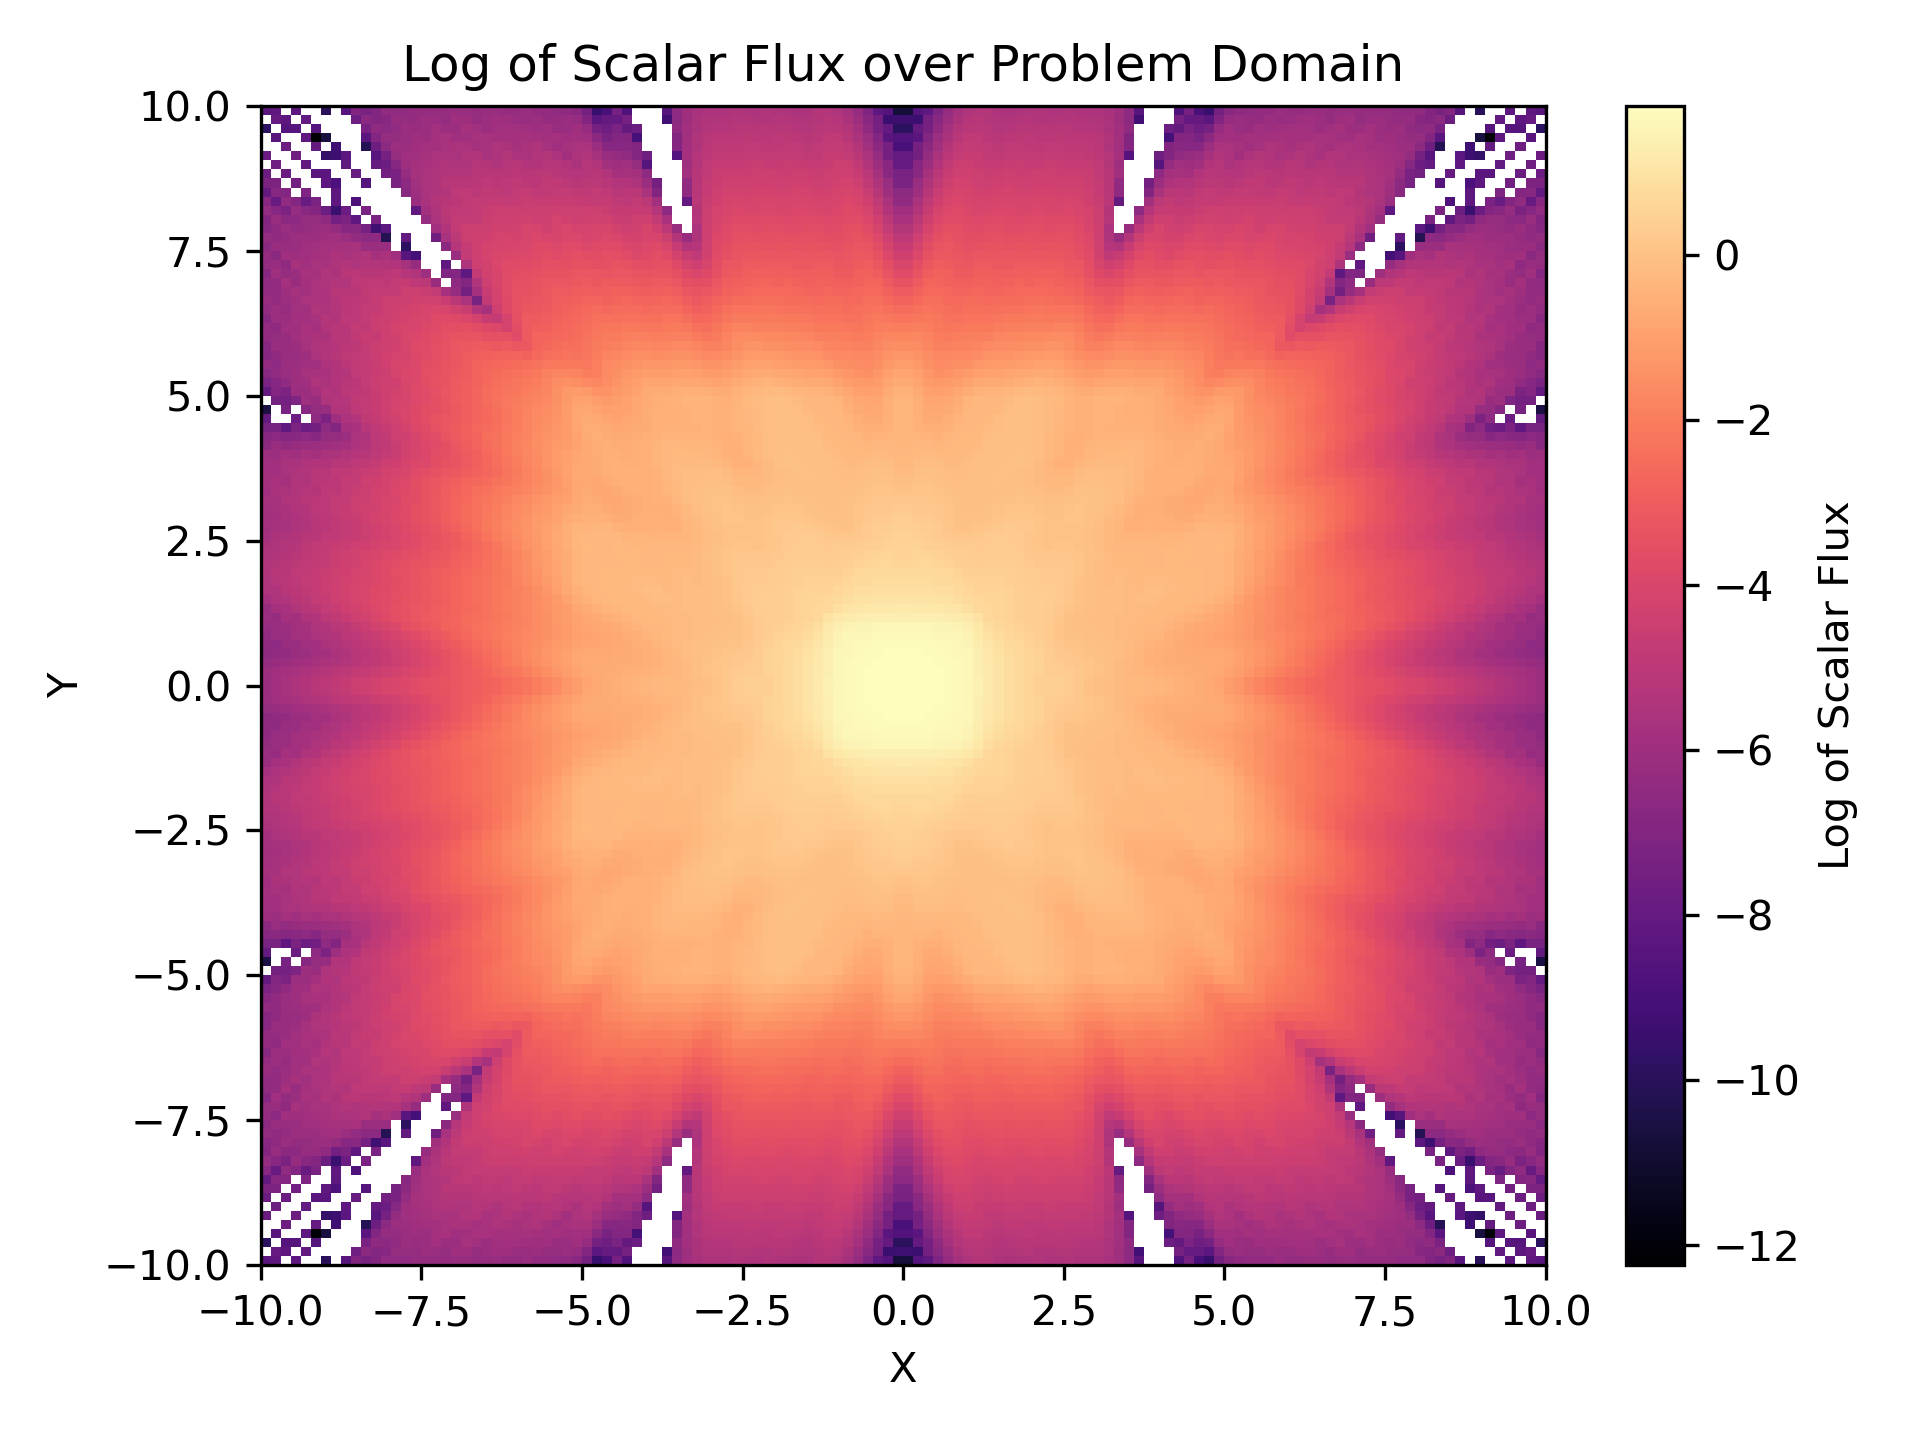
\includegraphics[width=0.65\textwidth]{figures/absorbing/cell_fluxes_16384_8_log.png}
      \subcaption{$N=16384$, $S_{8}$}
    \end{subfigure}%
    \begin{subfigure}{.5\textwidth}
      \centering
      
\includegraphics[width=0.65\textwidth]{figures/scattering/cell_fluxes_16384_8_log.png}
      \subcaption{$N=16384$, $S_{8}$}
    \end{subfigure}
    \caption{Log scale of \glspl{arp1} problem highlighting ray effects.}
  \end{figure}
\end{frame}


\begin{frame}
  \frametitle{\glspl{arp1} Comparison with Paper}
  \begin{figure}[b]
    \centering
    \begin{subfigure}{.5\textwidth}
      \centering
      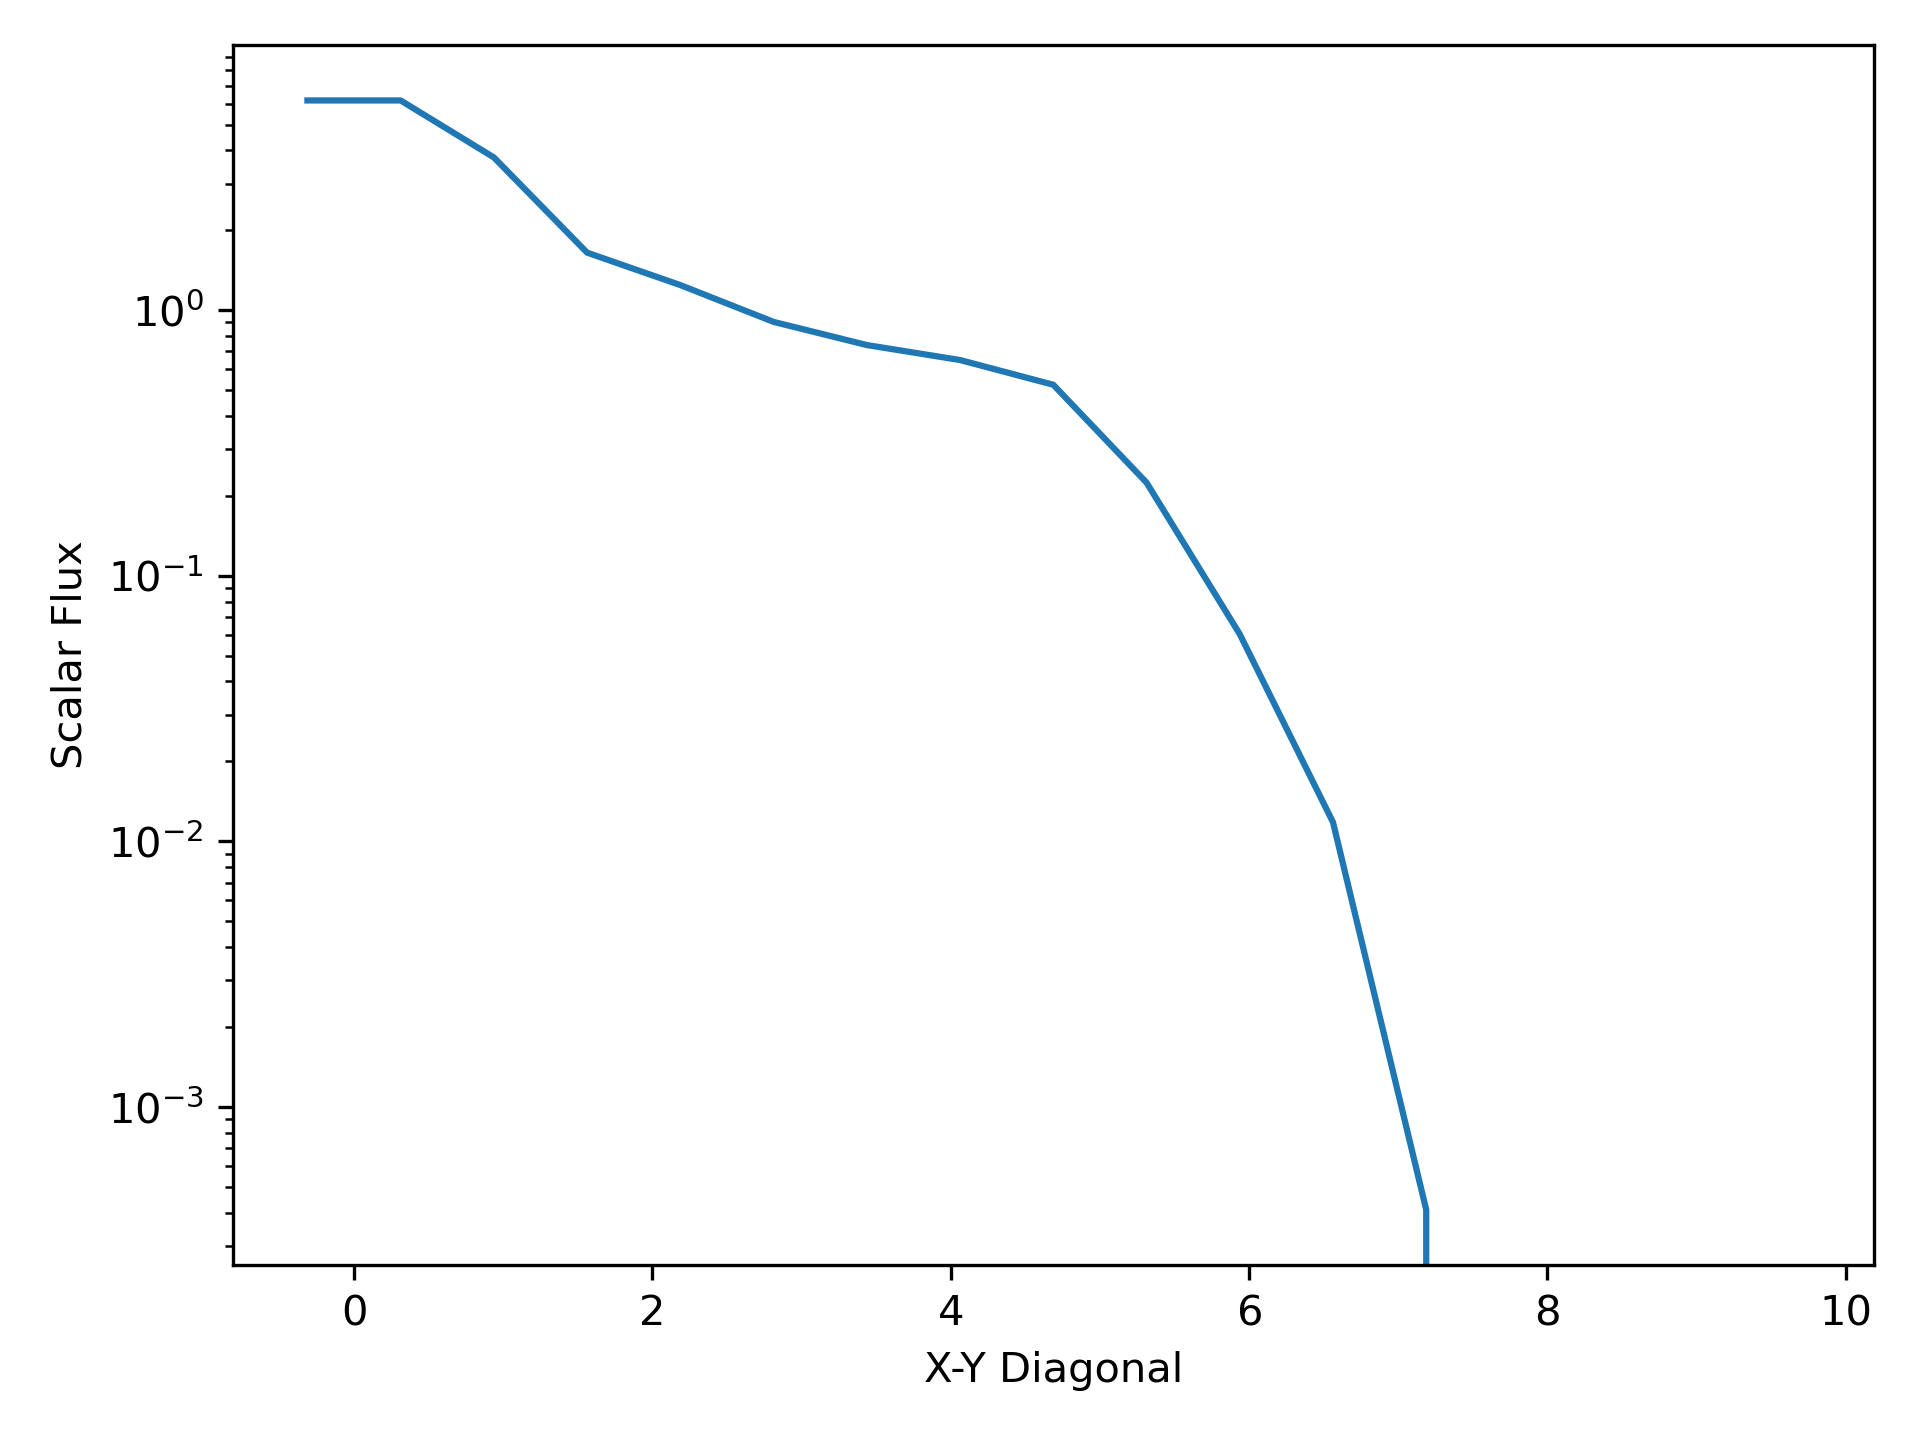
\includegraphics[width=0.65\textwidth]{figures/absorbing/diagonal_flux_1024_8.png}
      \subcaption{$N=1024$, $S_{8}$}
    \end{subfigure}%
    \begin{subfigure}{.5\textwidth}
      \centering
      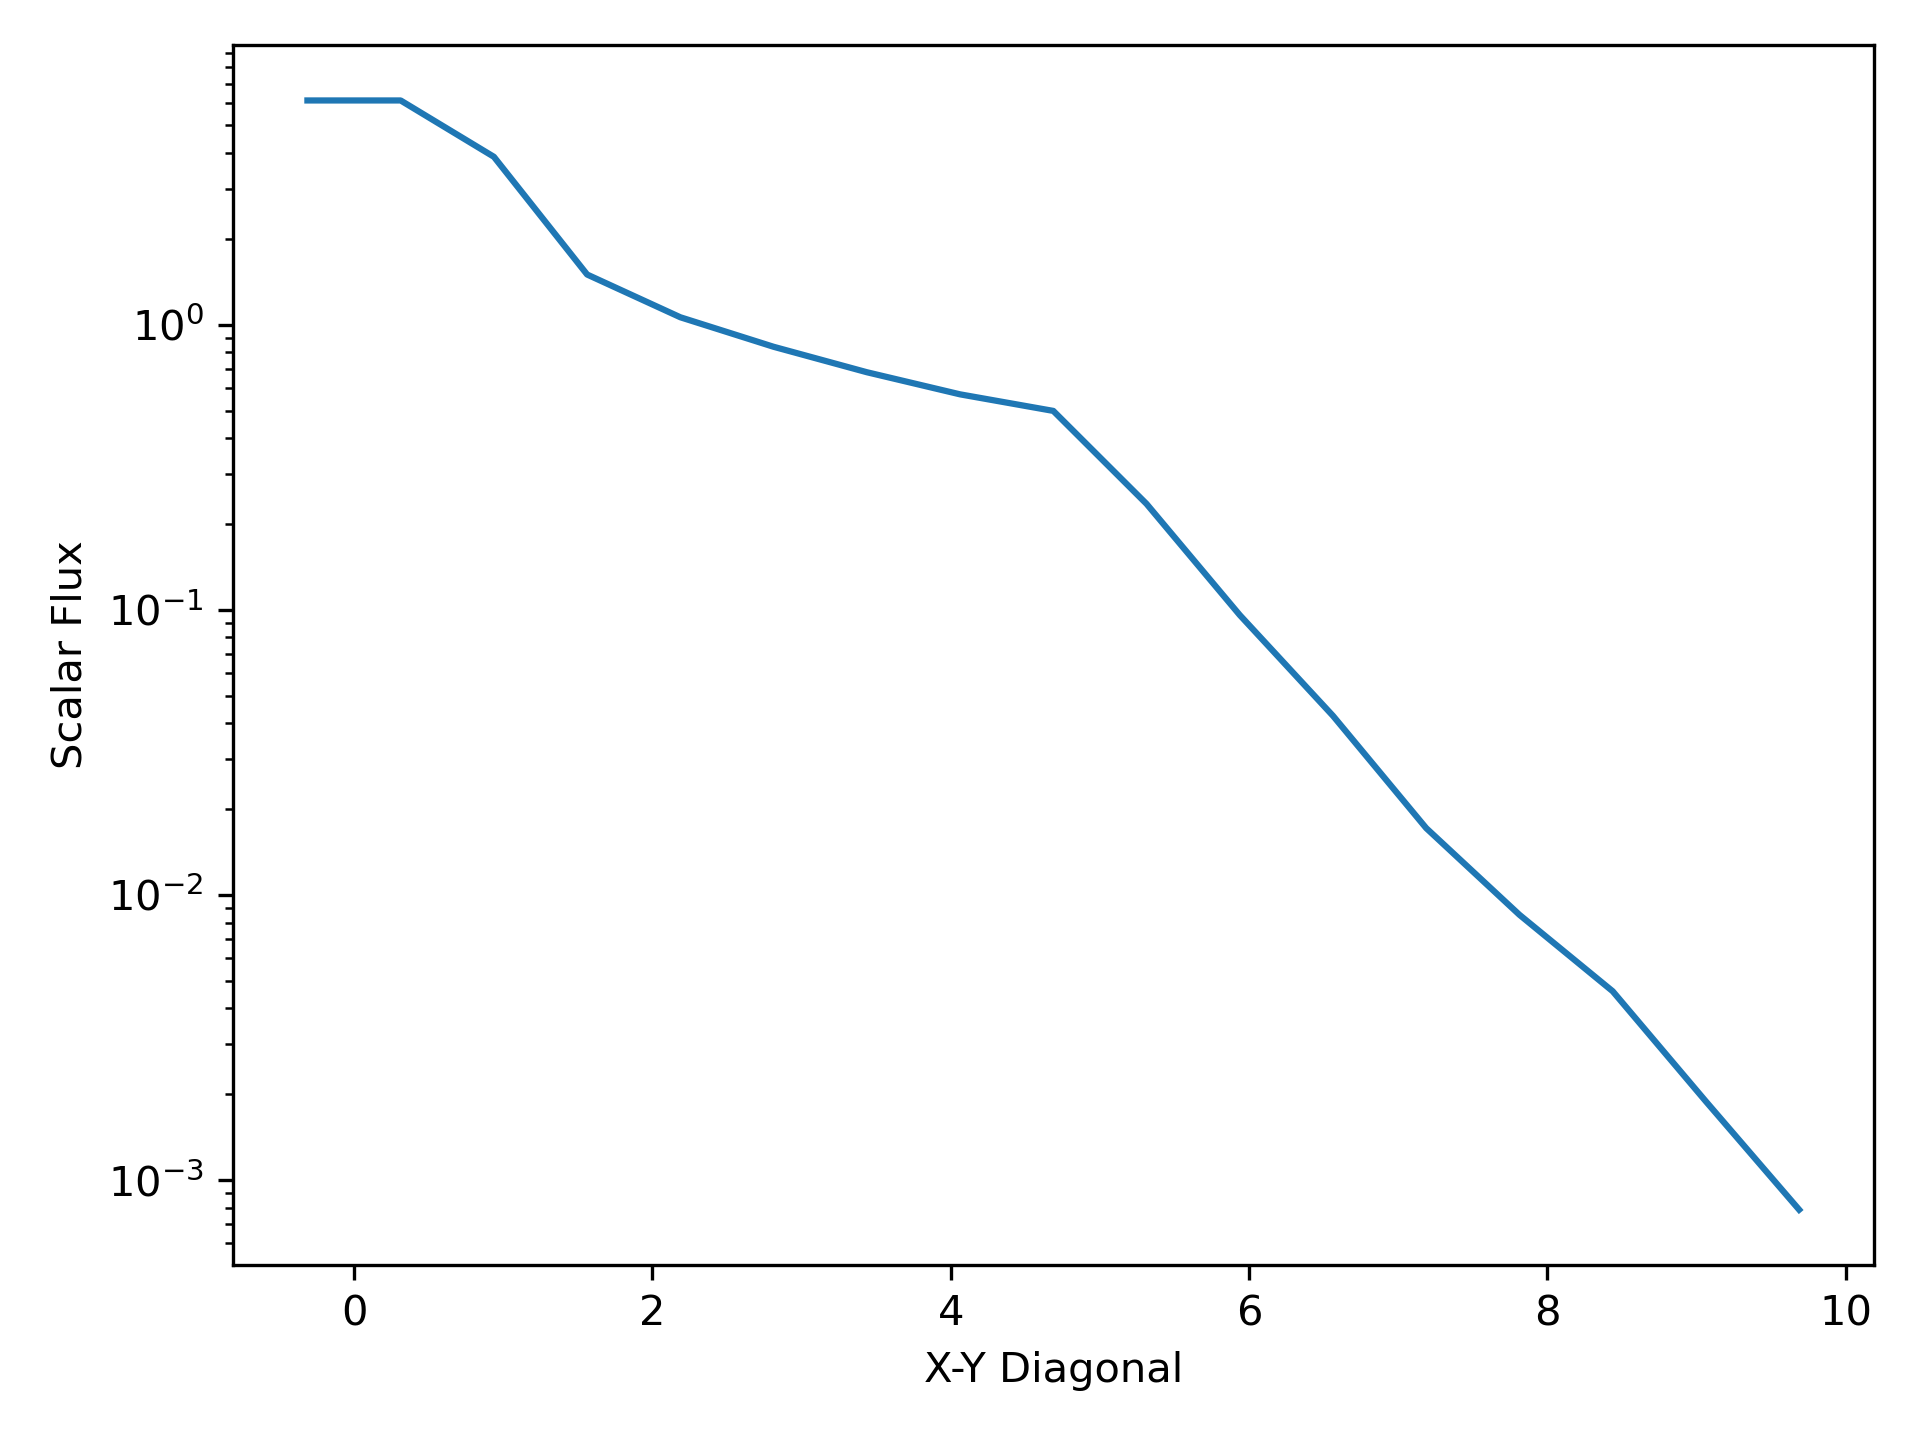
\includegraphics[width=0.65\textwidth]{figures/absorbing/diagonal_flux_1024_32.png}
      \subcaption{$N=1024$, $S_{32}$}
    \end{subfigure}
    \begin{subfigure}{.5\textwidth}
      \centering
      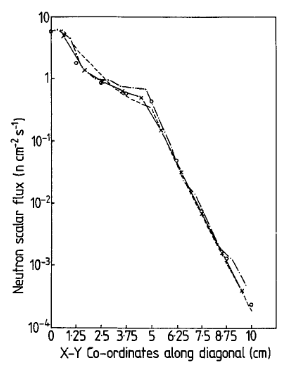
\includegraphics[width=0.5\textwidth]{figures/arp1_paper_result.png}
      \subcaption{Flux along diagonal for three different solution techniques.}
    \end{subfigure}%
    \caption{Comparison of \glspl{arp1} solutions with original paper.}
  \end{figure}
\end{frame}


\begin{frame}
  \frametitle{\glspl{arp} "Straight Duct" Problem}
  \begin{figure}[b]
    \centering
    \begin{subfigure}{.5\textwidth}
      \centering
      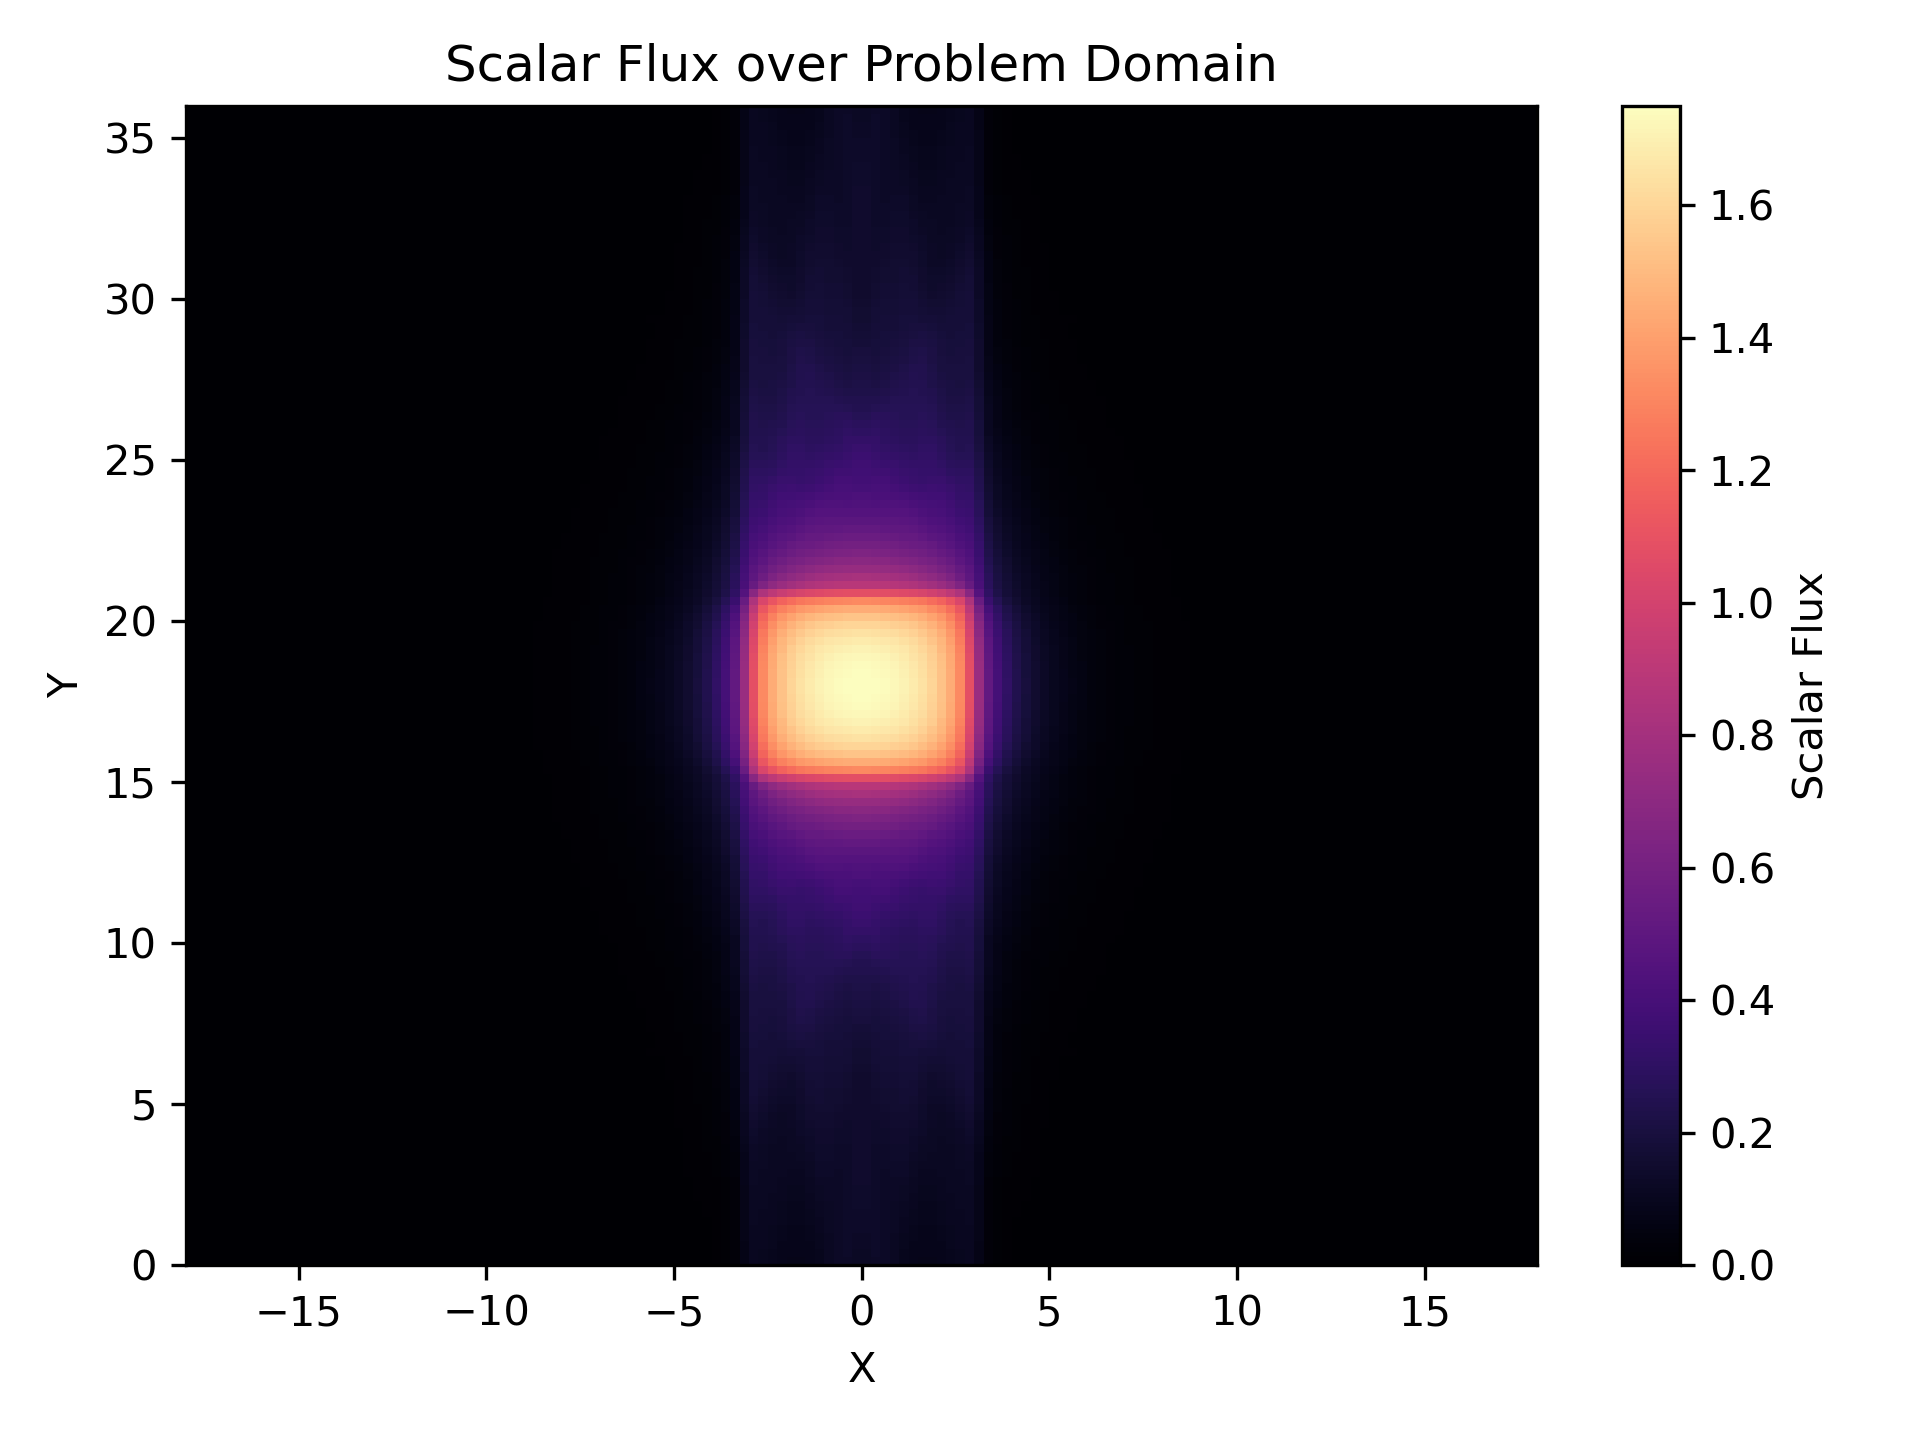
\includegraphics[width=0.65\textwidth]{figures/other_problems/absorb_duct_20736_16.png}
      \subcaption{Absorbing Medium}
    \end{subfigure}%
    \begin{subfigure}{.5\textwidth}
      \centering
      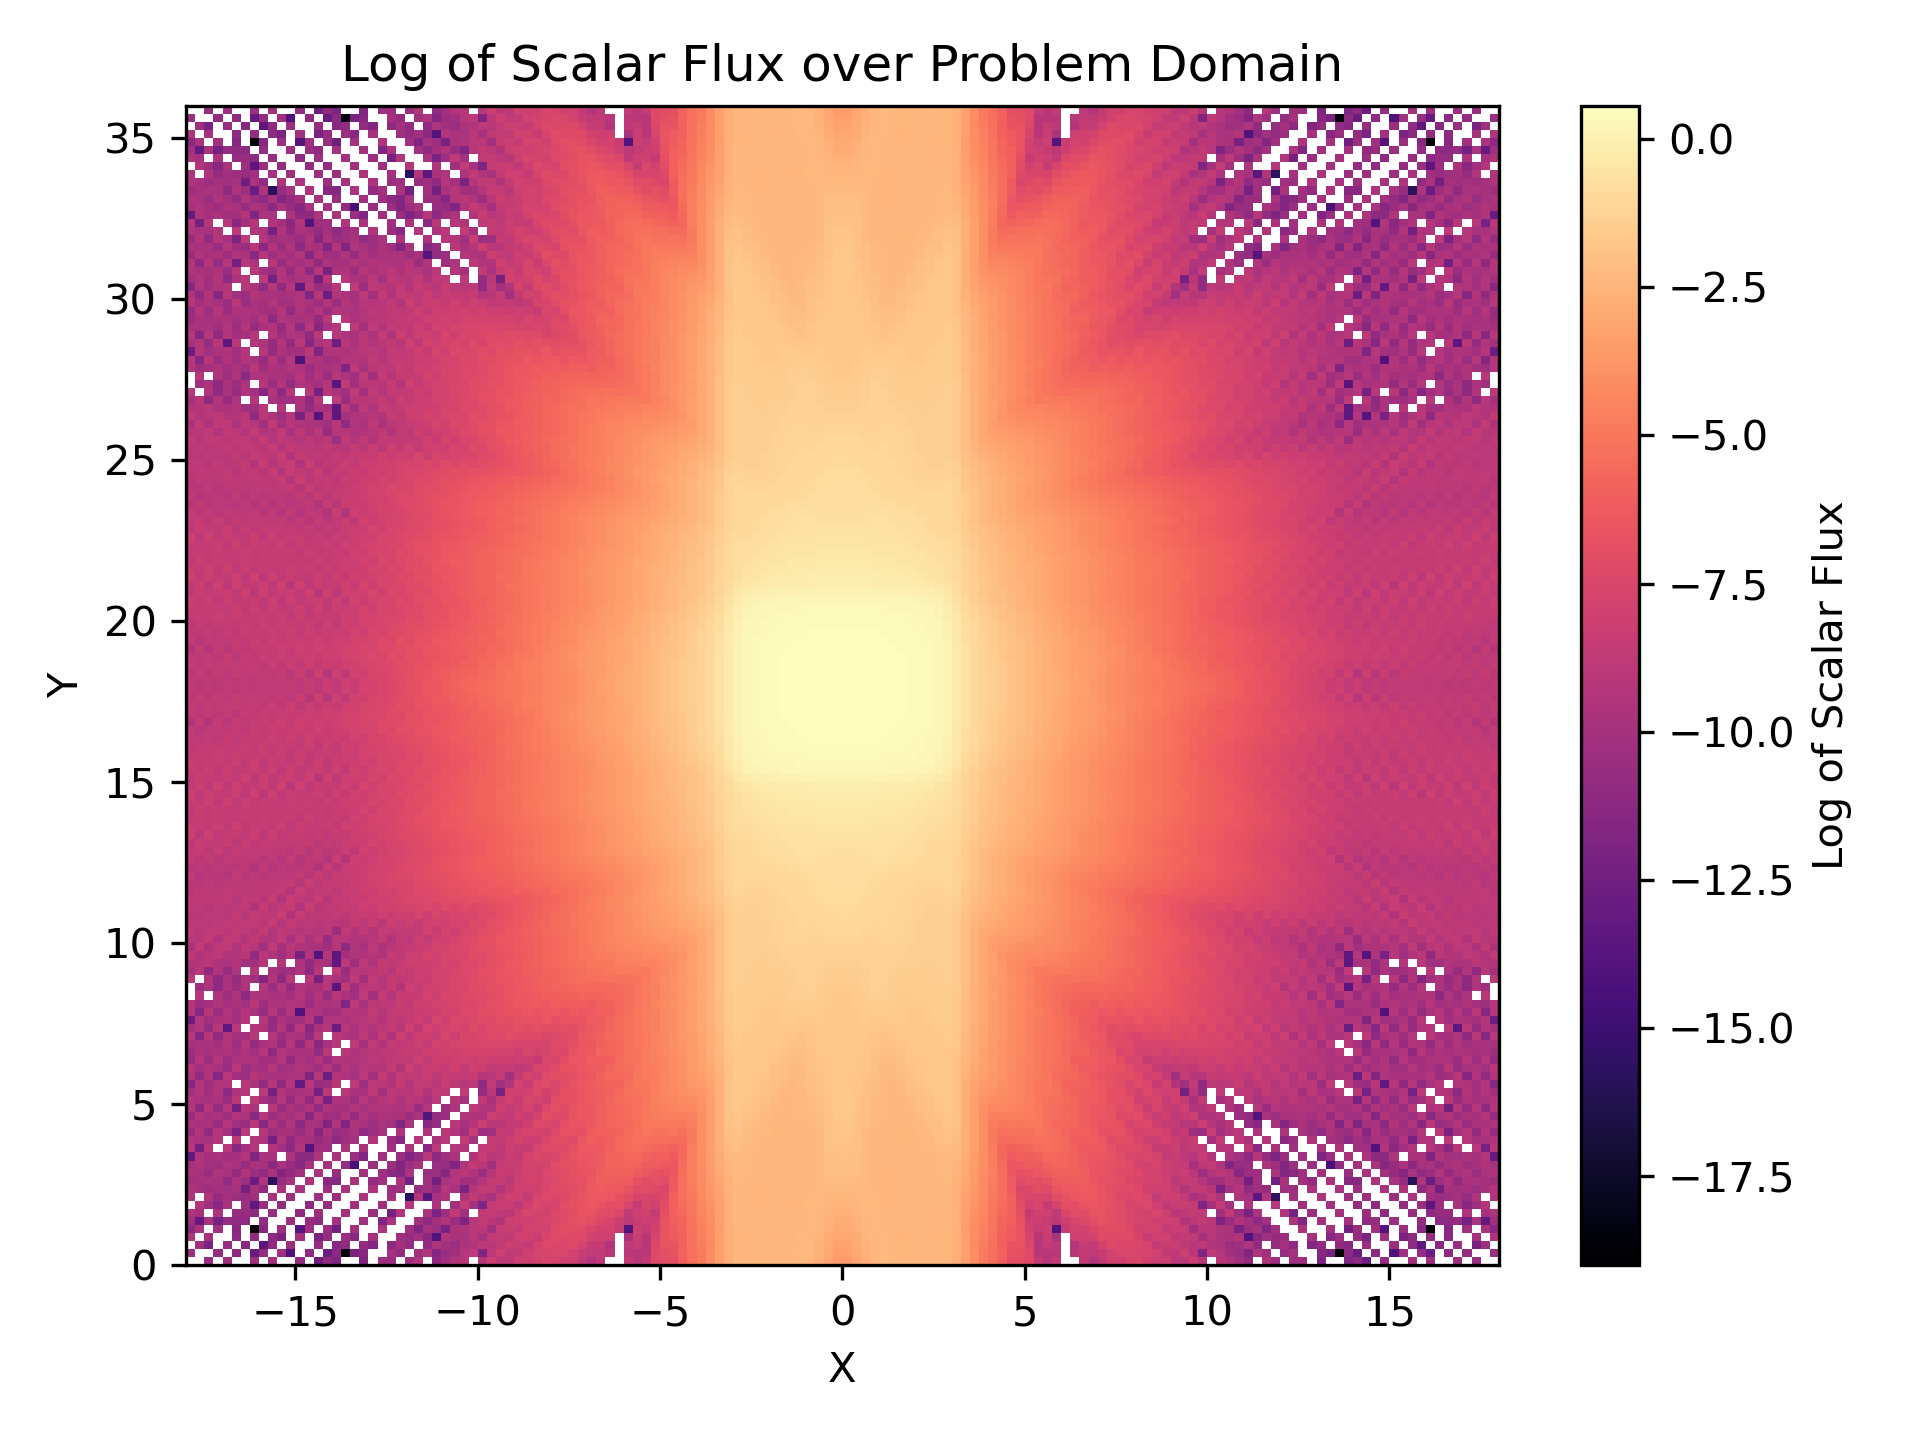
\includegraphics[width=0.65\textwidth]{figures/other_problems/absorb_duct_log.png}
      \subcaption{Absorbing Medium, Log Scale}
    \end{subfigure}
    \begin{subfigure}{.5\textwidth}
      \centering
      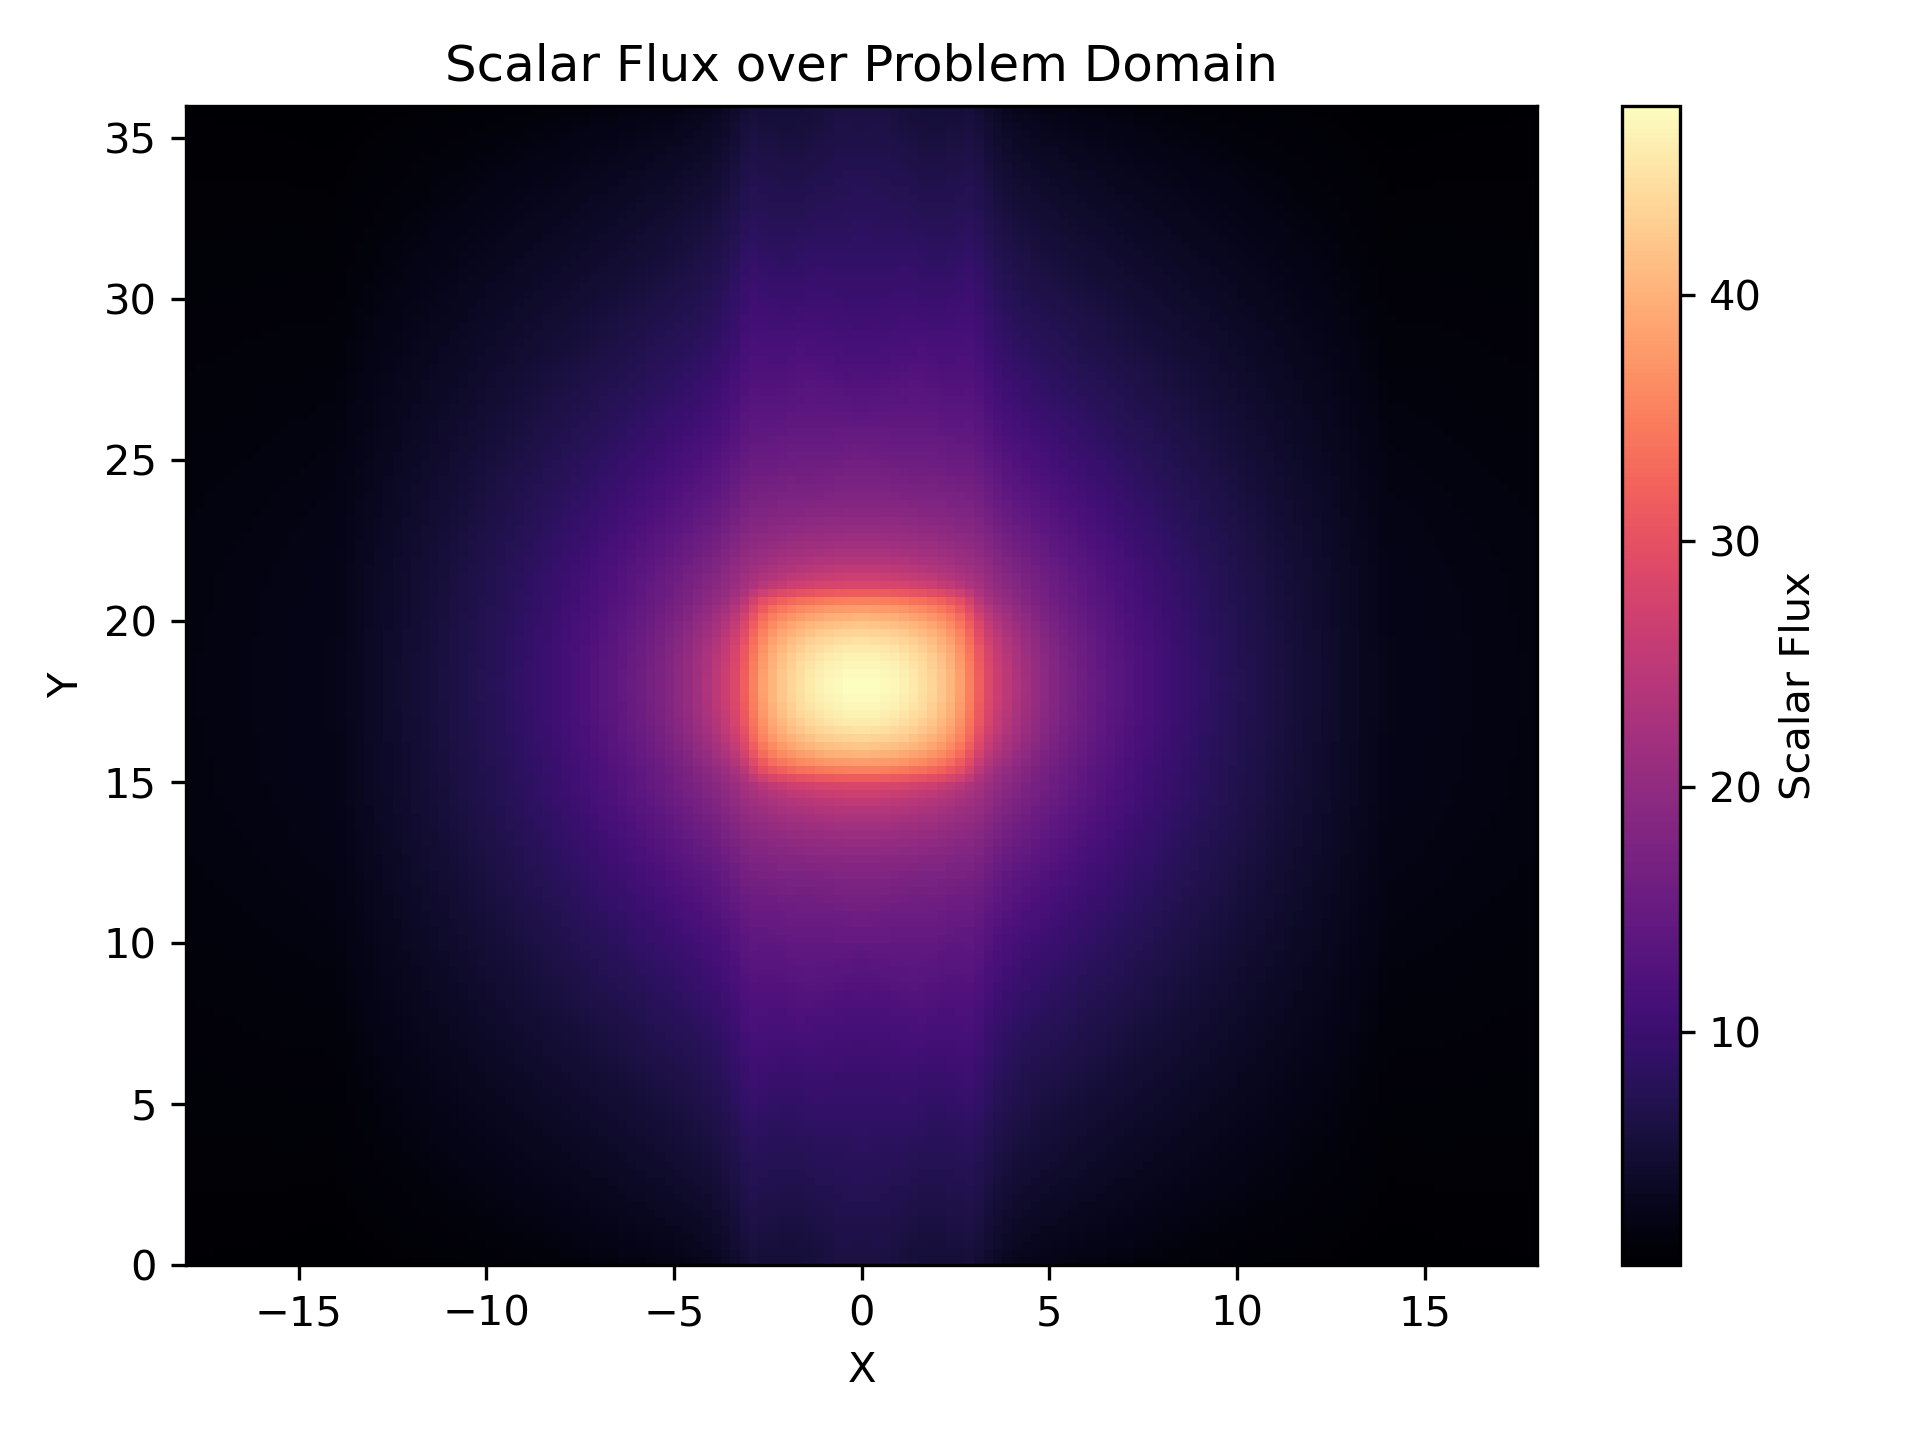
\includegraphics[width=0.65\textwidth]{figures/other_problems/scatter_duct_20736_16.png}
      \subcaption{Scattering Medium}
    \end{subfigure}%
    \begin{subfigure}{.5\textwidth}
      \centering
      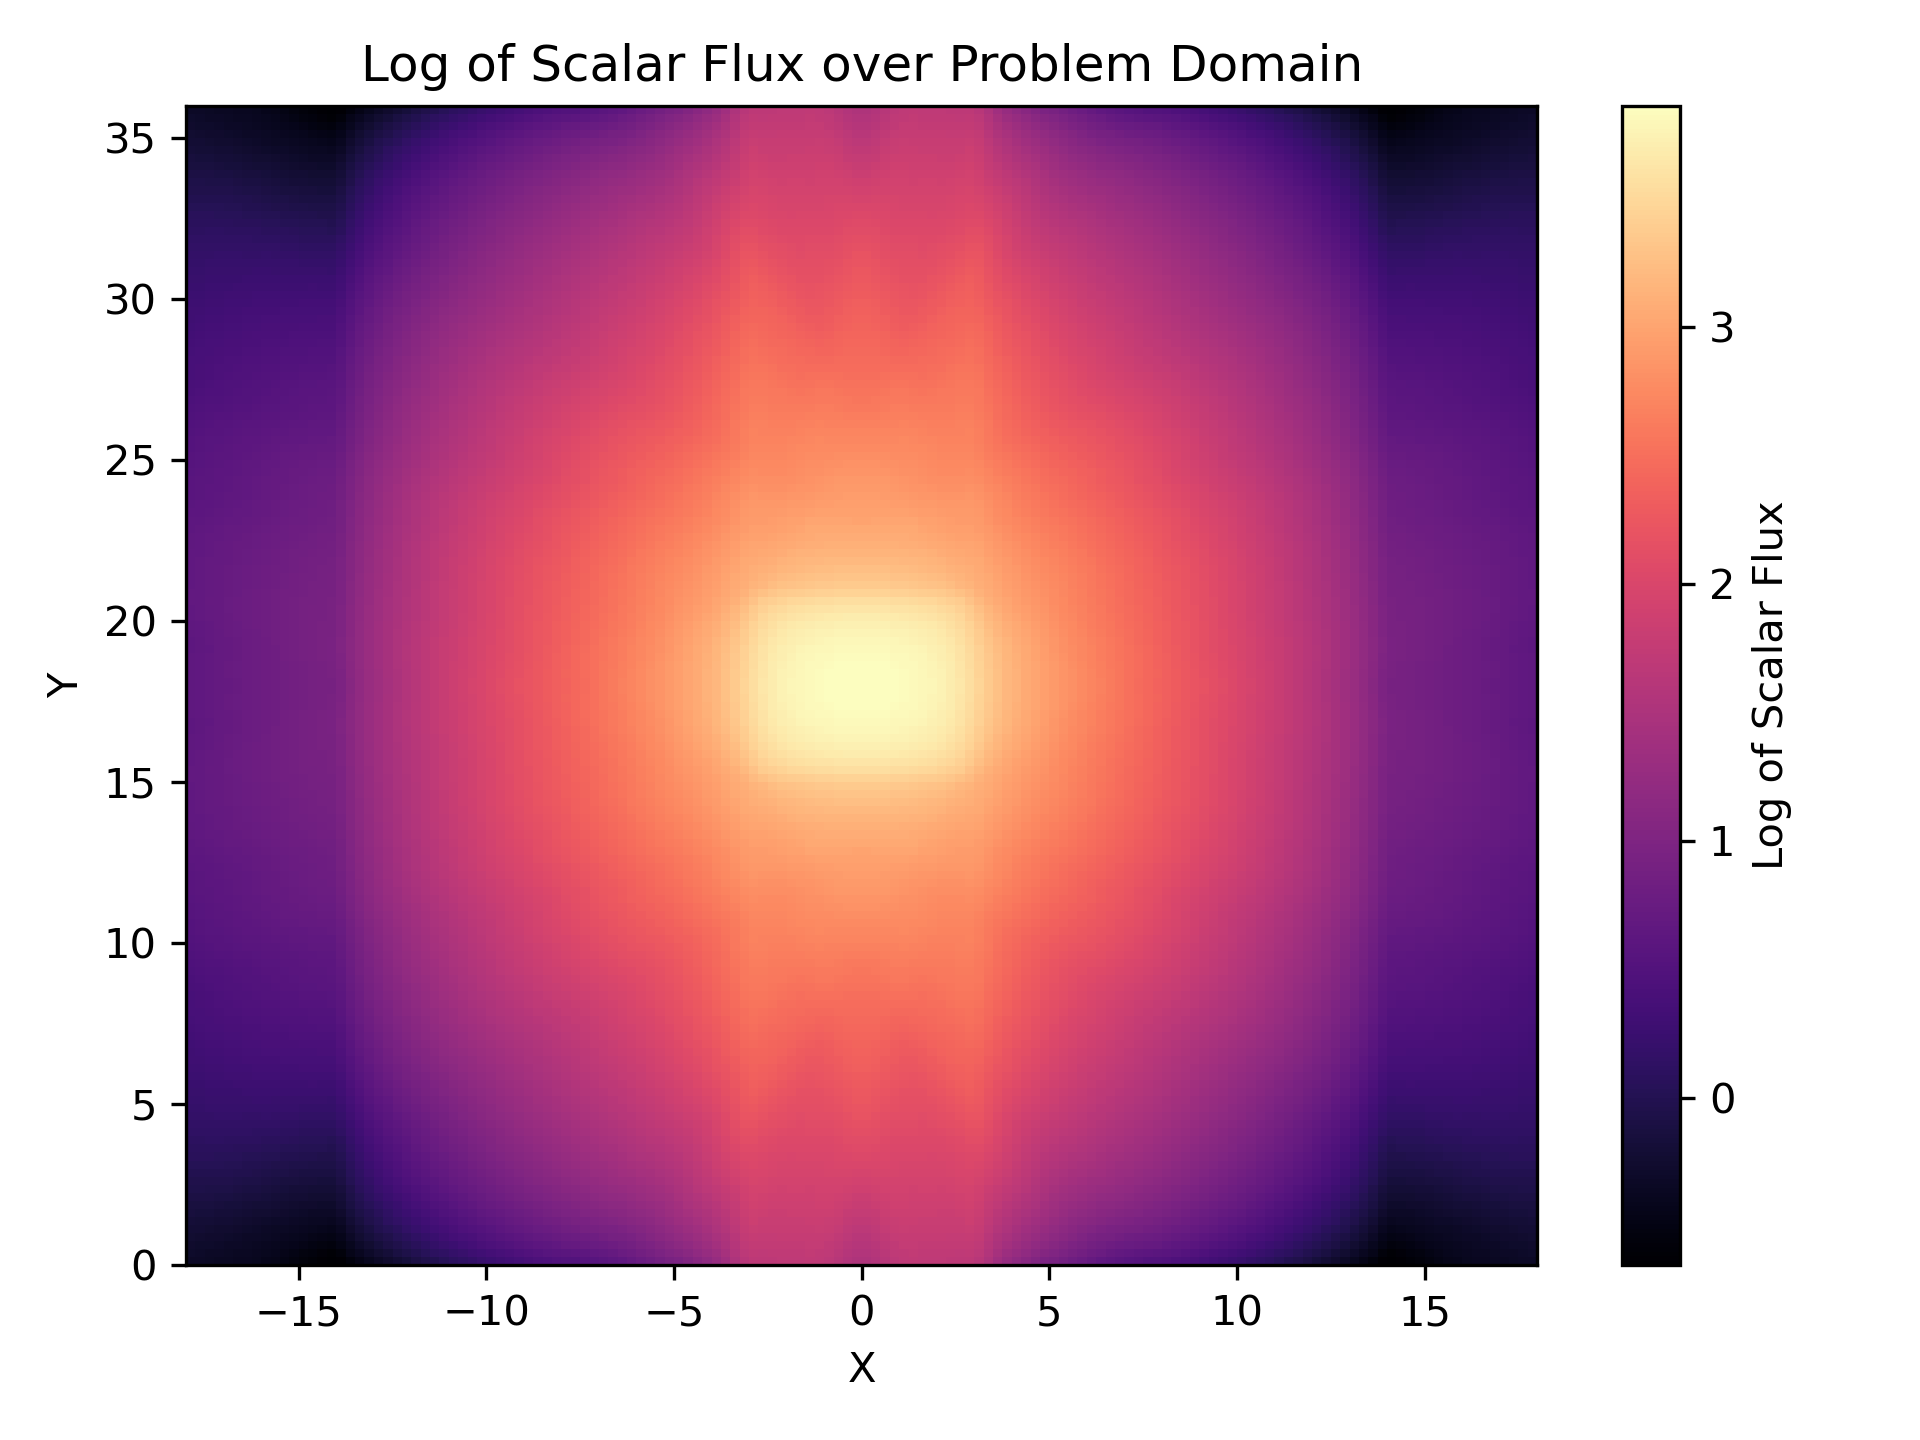
\includegraphics[width=0.65\textwidth]{figures/other_problems/scatter_duct_log.png}
      \subcaption{Scattering Medium, Log Scale}
    \end{subfigure}
    \caption{Solutions of \glspl{arp} duct problem for $N=20736$ and $S_8$.}
  \end{figure}
\end{frame}


\begin{frame}
  \frametitle{\glspl{arp} "Dog Leg" Problem}
  \begin{figure}[b]
    \centering
    \begin{subfigure}{.5\textwidth}
      \centering
      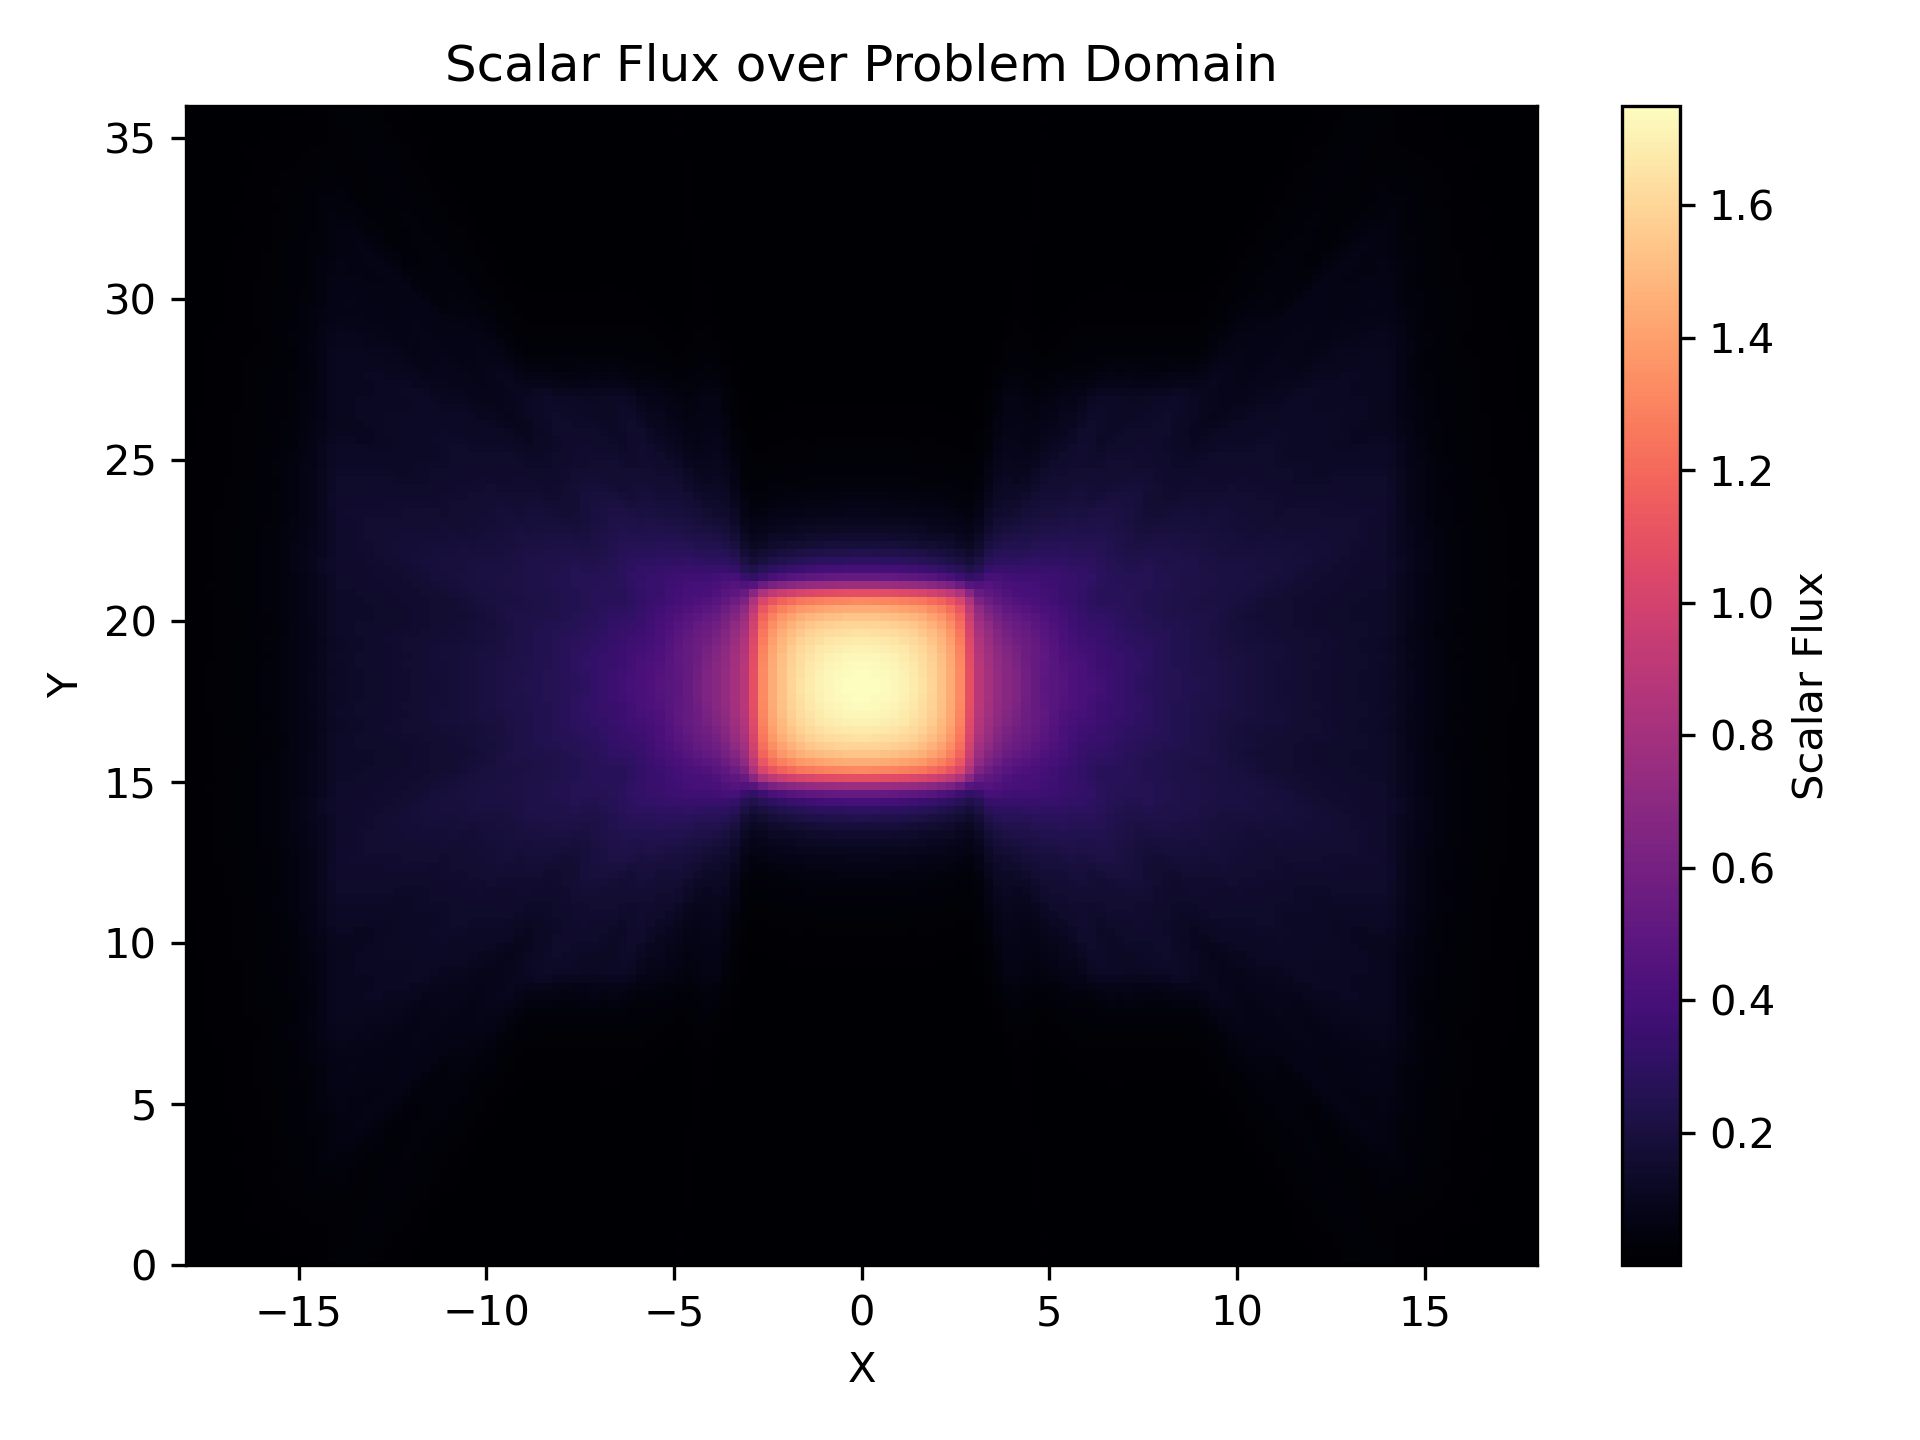
\includegraphics[width=0.65\textwidth]{figures/other_problems/absorb_dogleg_20736_16.png}
      \subcaption{Absorbing Medium}
    \end{subfigure}%
    \begin{subfigure}{.5\textwidth}
      \centering
      
\includegraphics[width=0.65\textwidth]{figures/other_problems/absorb_dogleg_log.png}
      \subcaption{Absorbing Medium, Log Scale}
    \end{subfigure}
    \begin{subfigure}{.5\textwidth}
      \centering
      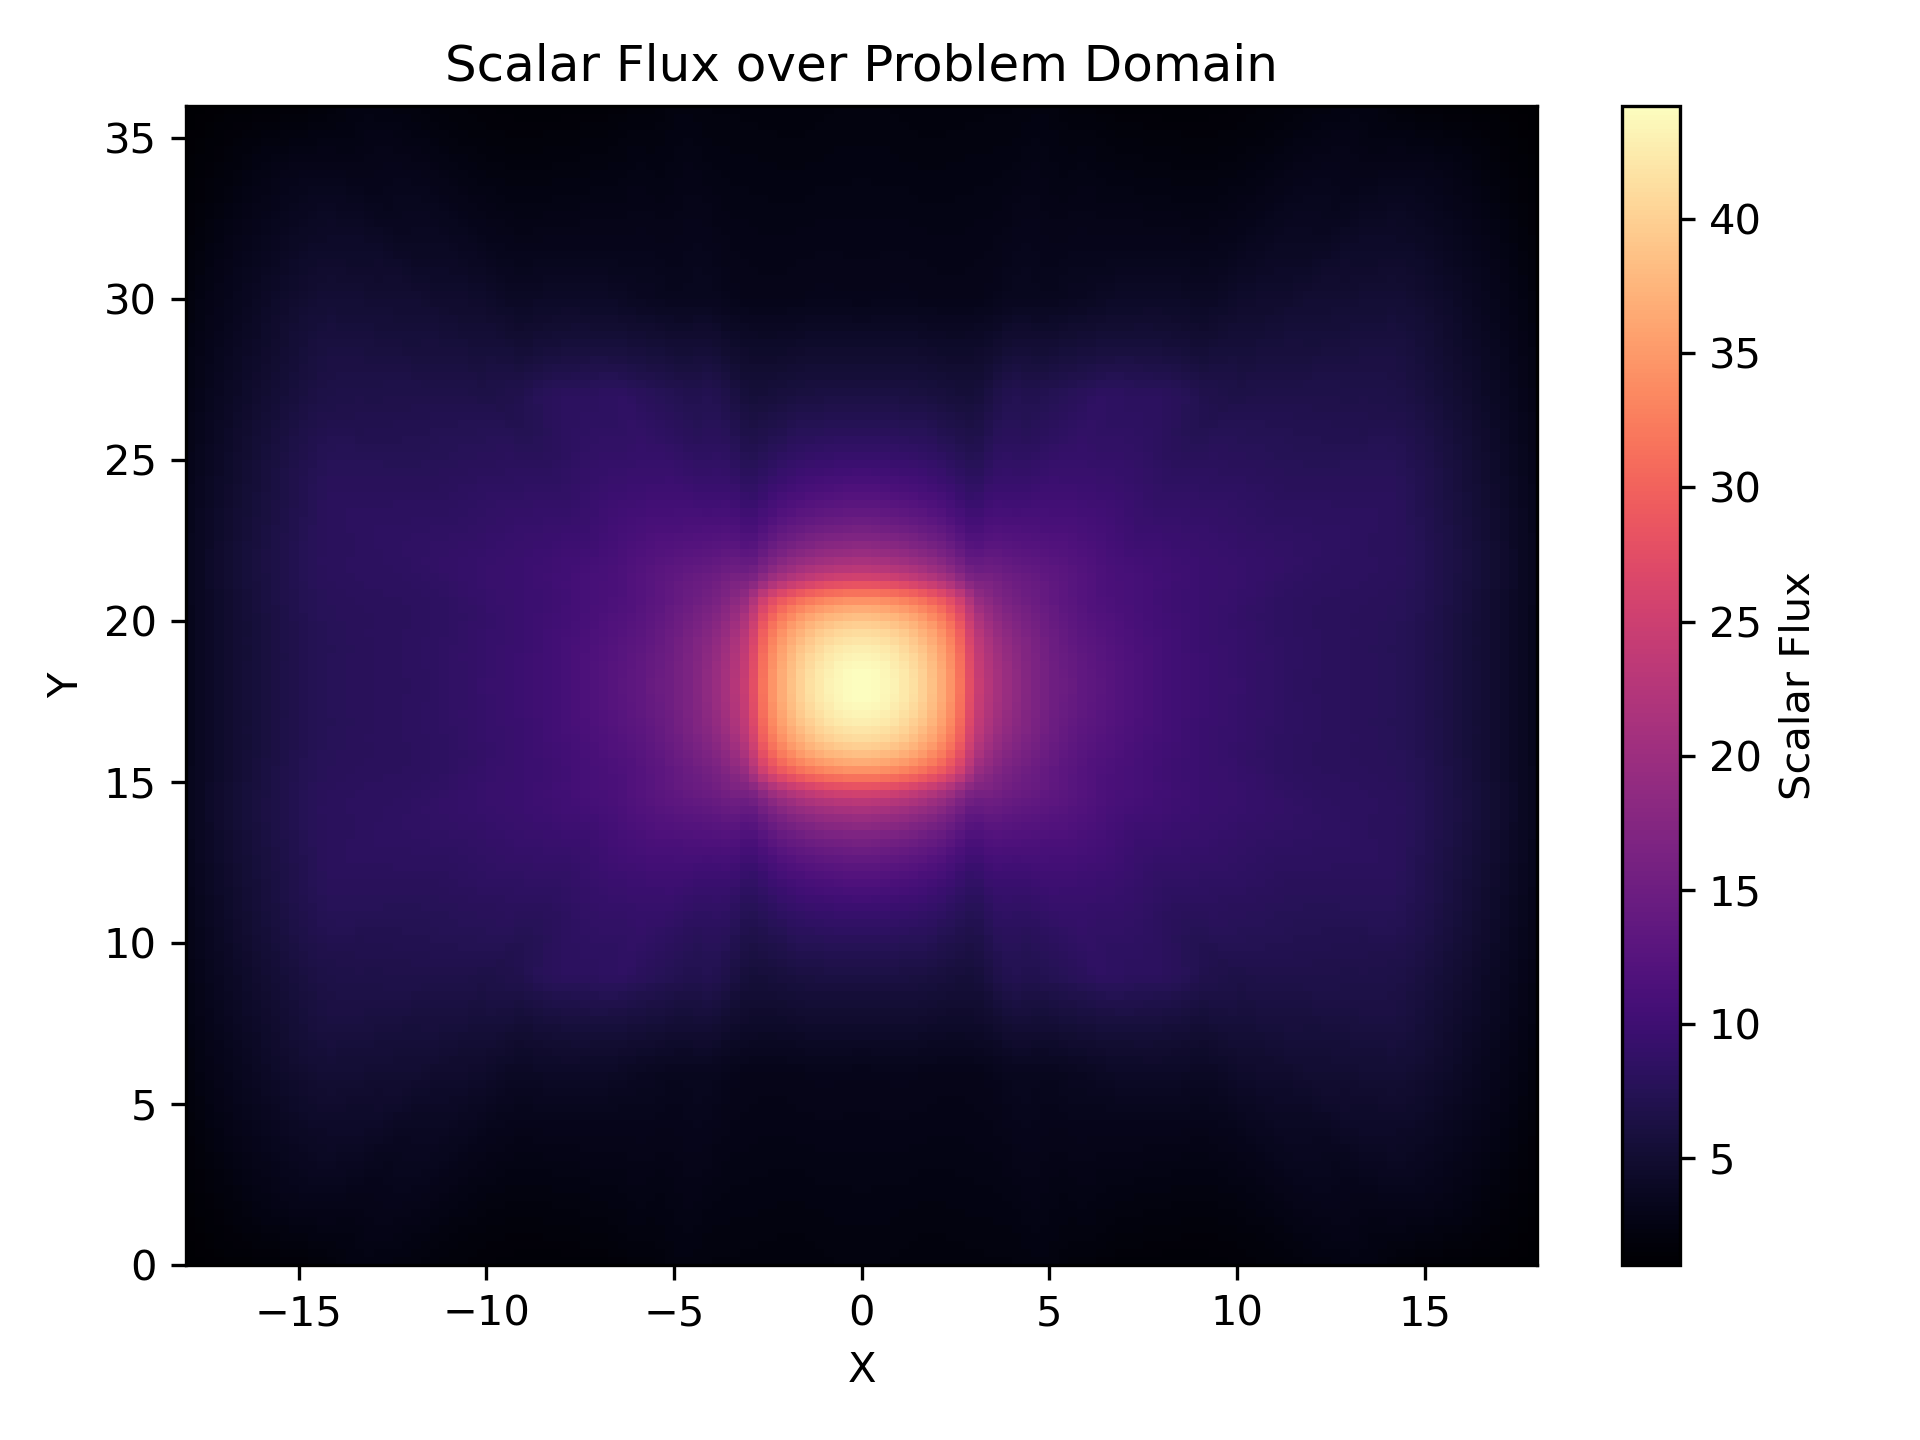
\includegraphics[width=0.65\textwidth]{figures/other_problems/scatter_dogleg_20736_16.png}
      \subcaption{Scattering Medium}
    \end{subfigure}%
    \begin{subfigure}{.5\textwidth}
      \centering
      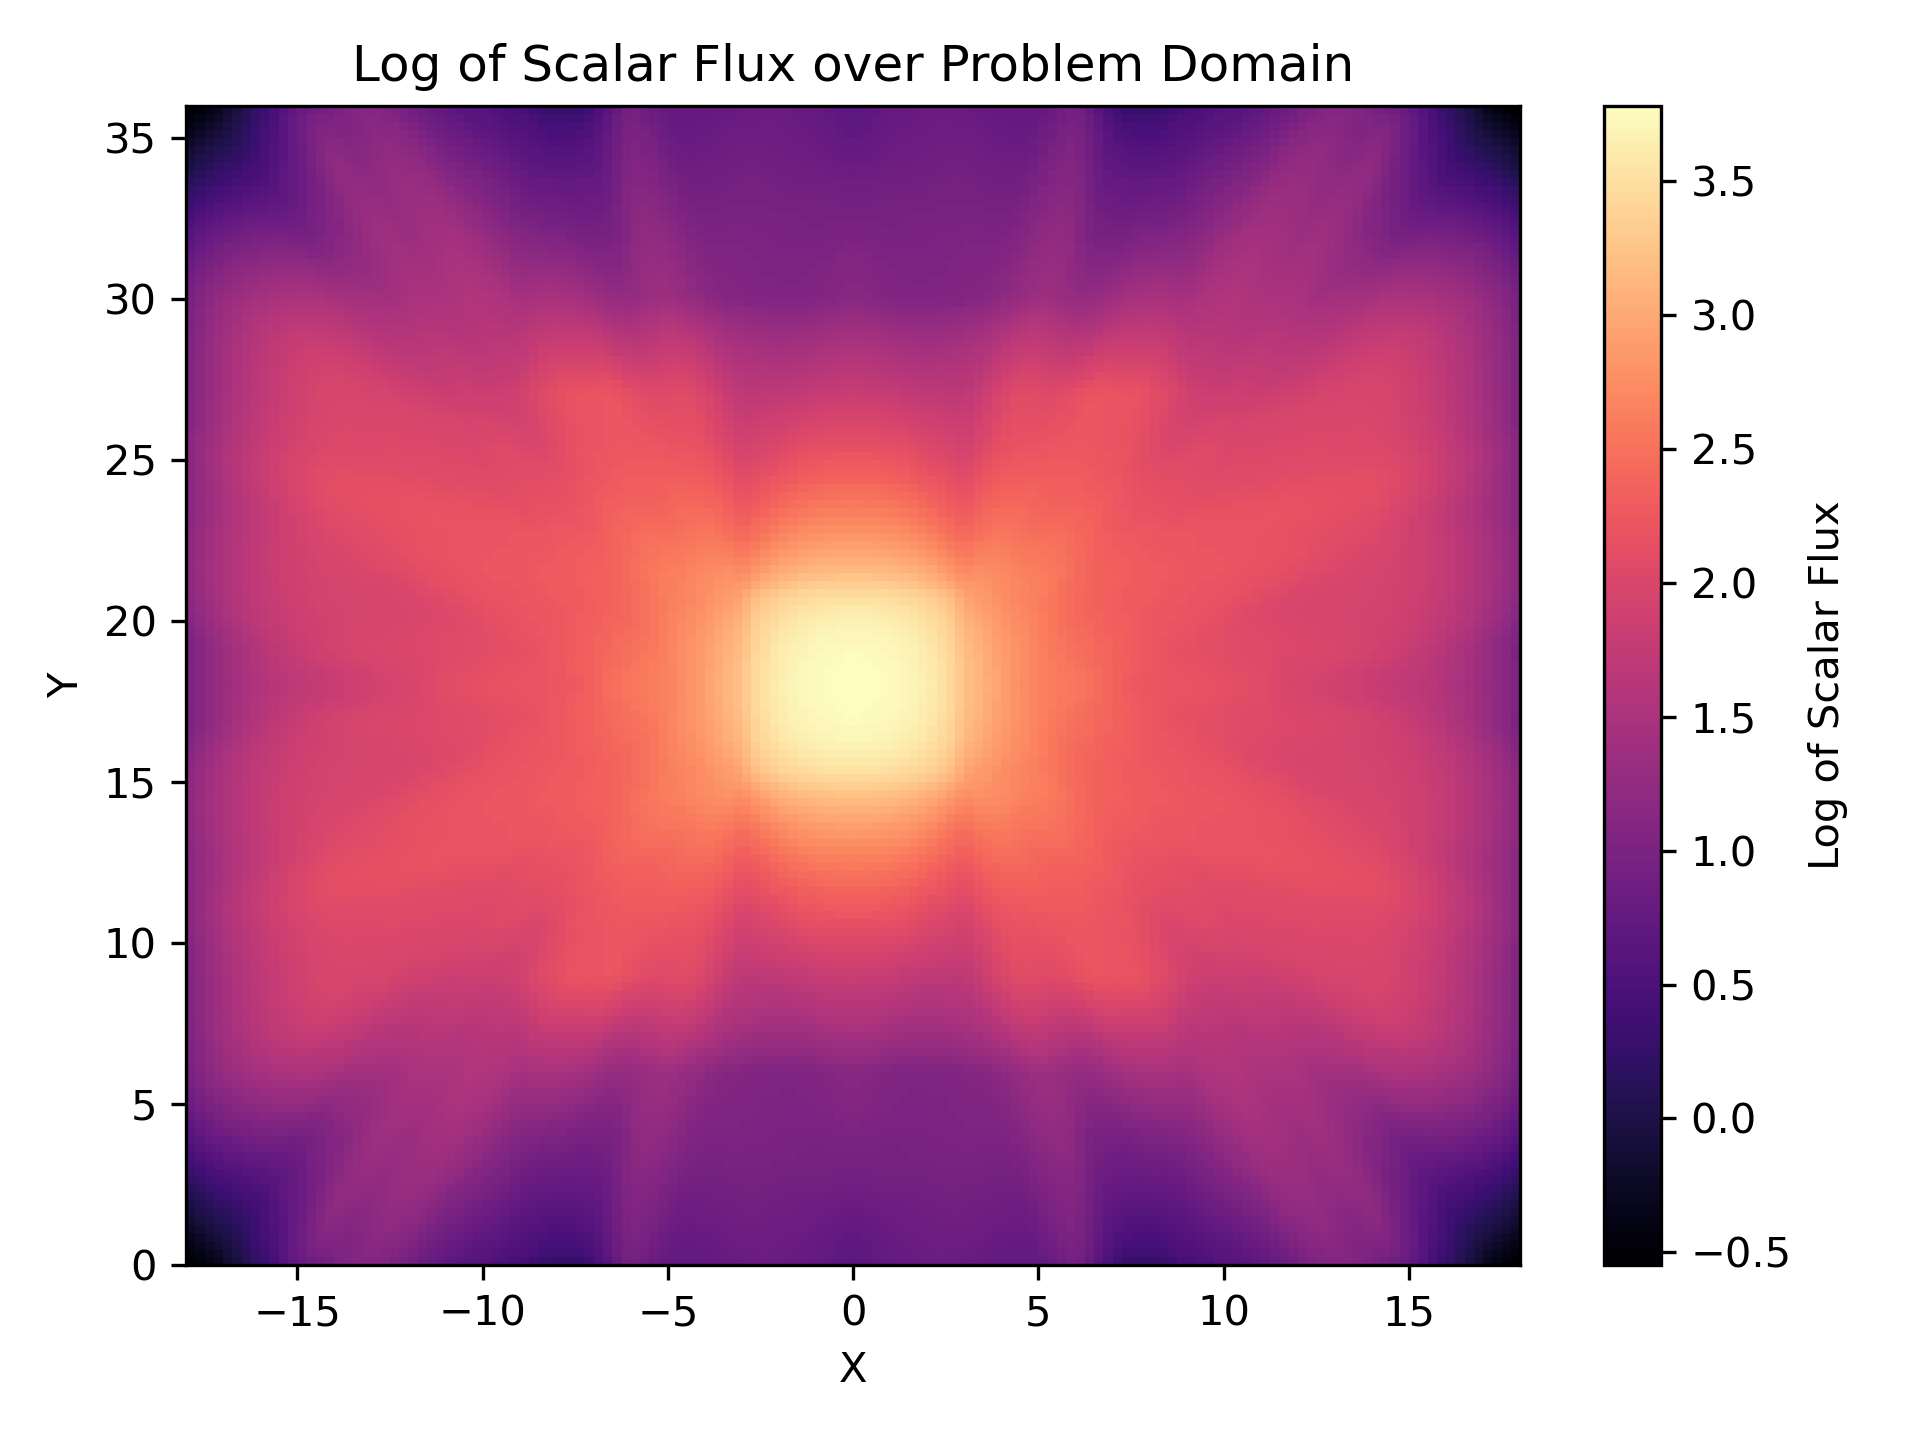
\includegraphics[width=0.65\textwidth]{figures/other_problems/scatter_dogleg_log.png}
      \subcaption{Scattering Medium, Log Scale}
    \end{subfigure}
    \caption{Solutions of \glspl{arp} dog leg problem for $N=20736$ and $S_8$.}
  \end{figure}
\end{frame}
